%***************************************************************************
% 
% FR 卒業論文本稿 TeX フォーマット（横山研非公式2020/02/04）
% 
%***************************************************************************
\documentclass[a4j,11pt,onecolumn,oneside,fleqn,final]{sty_file/s_report}
\ifnum 42146=\euc"A4A2 \AtBeginDvi{\special{pdf:tounicode EUC-UCS2}}\else
\AtBeginDvi{\special{pdf:tounicode 90ms-RKSJ-UCS2}}\fi
\usepackage[dvipdfmx]{color}
\usepackage[dvipdfm,bookmarks=true,bookmarksnumbered=true,%
bookmarkstype=toc]{hyperref}
\usepackage[dvipdfmx]{graphicx}
\usepackage{amsmath,ascmac}
\usepackage{fancyvrb}
\usepackage{fancyhdr}
\usepackage{sty_file/eclbkbox}
\usepackage{ascmac}
\usepackage{sty_file/cprog}
\usepackage{lscape}
\usepackage{color}
\usepackage{multirow}
\usepackage{listings, sty_file/jlisting}
\usepackage{here}
\usepackage{amsmath}
%\usepackage{minted}

%==============自分で追加=============%


%---------プログラムリストの設定------------------
\renewcommand{\lstlistingname}{リスト}
\lstset{
	language=[ANSI]C,%
	breaklines=true, %折り返す
	tabsize=2,%タブサイズ
	basicstyle=\footnotesize,%
	firstnumber=0,
	%commentstyle=\textit,%
	%keywordstyle=\bfseries,
	commentstyle={\small\ttfamily \color[rgb]{0,0.5,0}},
	keywordstyle={\small\bfseries \color[rgb]{0,0,0.8}},%,% 
	directivestyle={\small\bfseries \color[rgb]{0,0,0.8}},
	frame=single,
	framesep=5pt,%
	showstringspaces=false,%
	linewidth=420pt,%全体の幅
	numbersep=10pt, %行番号と本文の間隔（default=10pt)
	breakindent=5pt, %自動改行後のインデント(default=20pt)
	numbers=left, %行番号を左に付ける
	stepnumber=10,
	numberstyle=\footnotesize,%
	classoffset=1,%
}
%----------ここまでプログラムリストの設定-----------------
\def\ProgList#1{\fvset{fontsize=\footnotesize, baselinestretch=0.7, tabsize=4, numbers=left, stepnumber=5} \VerbatimInput{#1}}

\pagestyle{fancy}
\lhead{\leftmark}
\chead{}
\rhead{\rightmark}
\lfoot{}
\cfoot{--\thepage{}--}
\rfoot{}
\renewcommand{\headrulewidth}{0.4pt}
\renewcommand{\footrulewidth}{0.4pt}

\setcounter{topnumber}{6}		% ページ上部の最大フロート数
\def\topfraction{1.00}			% ページ上部のフロートで占める最大の割合
\setcounter{bottomnumber}{6}	% ページ下部の最大フロート数
\def\bottomfraction{1.00}		% ページ下部のフロートで占める最大の割合
\setcounter{totalnumber}{12}	% 1ページの最大フロート数
\def\textfraction{0.08}			% 1ページのテキスト部の占める最小割合
\def\floatpagefraction{0.7}		% フロートが単独ページになるときの最小割合

\title{\vspace{-20mm}{\Large 令4年度\\\ 卒\ 業\ 論\ 文} \vspace{15mm}\\
連系リアクトルなし三相系統連系システムの\\ロバスト性の検証\vspace{50mm}}
\author{指導教員~~~~横山 智紀　教授 \vspace{10mm}\\ 東京電機大学　未来科学部　ロボット・メカトロニクス学科 \\  19FR053~~~~窪慎之助}
\date{}

\setcounter{secnumdepth}{3}%章節コマンドのカウンタ
\setcounter{tocdepth}{3}

%***************************************************************************
%******************　　　　　　以下，導入部　　　　　　　 ******************
%***************************************************************************
\begin{document}
\maketitle

%***************************************************************************
% Abstract 
%***************************************************************************
\begin{abstract}

現在の地球環境は気候変動問題に見舞われている．その対応として，パリ協定が2020年から本格利用を開始して以降，各国が2050年のカーボンニュートラルの実現に向けて取り組みを行っている．日本においても2050年までのカーボンニュートラルを目標とし，様々な取り組みを進めている．特に，国内の二酸化炭素の排出量の約40\%が電力に関する排出であることから，再生可能エネルギーの普及は日本の脱炭素社会の実現のために重要視されている\cite{1}\cite{2}．そのため，近年では分散型発電システムの普及が進んでいるが，一方で分散型発電システムは系統事故が発生した場合，電力系統に悪影響に悪影響を及ぼす可能性がある．そのため，系統連系インバータには定常応答時の安定性や系統事故時の運転継続性能といったFault Ride Through(FRT)要件を満たす高い制御性能が求められている．\par

先行研究から系統連系インバータに対してFPGAの高速演算能力を用いてシングルレートデッドビート制御(SRDB)やマルチサンプリングデッドビート制御(MSSRDB)を適用することでPI制御に比べて優れた制御応答が得られることが判明している．\par

大規模太陽光発電システムにおいて，太陽電池モジュールは系統連系インバータ，フィルタからなる電力変換器，連系リアクトル相当となるトランス盤を介して系統に接続されている．従来の大規模太陽光発電システムは製品として電力変換器，トランス盤を提供していた．そのため，デッドビート制御による系統連系インバータの電力制御に系統電圧や連系リアクトルの値を用いて制御式を構成することが可能であった．

一方で本稿で対象とする大規模太陽光発電システムは製品として提供するものにトランス盤が含まれていないものである．そのため，連系リアクトルは各需要家に存在するトランス盤内のリアクトルとなり，リアクトルの値を取得することが困難となっている．このことから，デッドビート制御による系統連系インバータの電力制御に連系リアクトルや系統電圧を含まずに制御式を構成する必要がある．\par

本稿では連系リアクトルを含まない三相系統連系システムにおいて，シングルレートデッドビート制御，マルチサンプリングデッドビート制御を制御手法として用いる．定常運転時と系統電圧が80\%瞬時低下した場合を模擬した系統擾乱発生時のシミュレーションを行う．そのとき，システムのパラメータを変更していないノミナル時の検証とパラメータを大きくした場合と小さくした場合のアンノミナル検証の比較を行うことで制御手法，パラメータを変更した場合でシステムのロバスト性がどのように変化するかを検証する．

\end{abstract}


%***************************************************************************
\tableofcontents % 目次出力
%***************************************************************************

%***************************************************************************
% Introduction 
%***************************************************************************
%Root main.tex
%---------------------------------------------------------------------------
%第1章　研究背景・目的
%---------------------------------------------------------------------------

\chapter{はじめに}
\label{chap:first}

\section{研究背景}
\subsection{系統連系システム}
日本は，すぐに使える資源に乏しく，国土を山と深い海に囲まれるなどの地理的制約を抱えており，
過去に幾度もエネルギー安定供給の危機に見舞われ，その都度，英知を結集してエネルギー安定供給の確保に取り組んできた．
しかし，2011年の東日本大震災および東京電力福島第一原子力発電所事故以降，原子力発電所の多くが停止した結果，
化石燃料に対する依存が高まり，その大宗を海外からの輸入に頼るという，エネルギー需給構造上の脆弱性が再び顕在化することとなった．

こうした中，2022年2月には，ロシアによるウクライナ侵略が発生し，日本を取り巻くエネルギー情勢は一変している．
エネルギー分野におけるインフレーションが世界的に顕著となり，国内でも電力需給ひっ迫やエネルギー価格の高騰が生じるなど，
石油危機以来のエネルギー危機が危惧される事態となった．
また2023年には，日本が原油の9割以上を依存する中東地域における軍事的な緊張が高まり，
化石燃料の調達に関する不確実性が上昇するなど，日本が抱えるエネルギー需給構造上の課題が改めて浮き彫りとなった．

エネルギーは国民生活や経済活動の基盤となるものであり，エネルギー安定供給が損なわれることは決してあってはならない．
化石燃料への過度な依存から脱却し，エネルギー危機にも耐え得るエネルギー需給構造への転換を進めていくためにも，
エネルギー安全保障に重点を置いた政策の再構築を進めることが強く求められている．

同時に，世界的な異常気象や大規模な自然災害が発生する中，世界では多くの国・地域が期限付きのカーボンニュートラル目標を表明し，
脱炭素に向けた機運は高い状態にある．こうした中，日本では，世界全体での1.5℃目標と整合的で，
2050年ネット・ゼロの実現に向けた直線的な経路にある野心的な目標として，
2035年度，2040年度に温室効果ガスを2013年度からそれぞれ60[\%]，73[\%]削減することを目指す新たな温室効果ガス削減目標を2025年2月に決定し，
気候変動問題に対して国家を挙げて対応する強い決意を表明した．\cite{ref00}．

再生可能エネルギーとして，太陽光発電は比較的リードタイムが短く，分散型エネルギーリソースとしての活用が期待されているため，
更なる導入拡大が見込まれている\cite{ref01}．
再生可能エネルギーは変動が大きく,その変動に合わせて最適な電力変換が必要である．
再生可能エネルギーの普及拡大に伴い，系統を安定化させることが求められている\cite{ref02}．

図\ref{Fig1.2}に系統連系のイメージ図を示す．
系統連系システムは，太陽光発電：Photo Voltaic(PV)，風力発電：Wind Tubuine(WT)といった分散型発電システムで発電した電力を火力発電や水力発電などの一極集中型発電システムにより発電した商用電力系統に接続するためのシステムである．
\newpage

\begin{figure}[ht]
    \center
    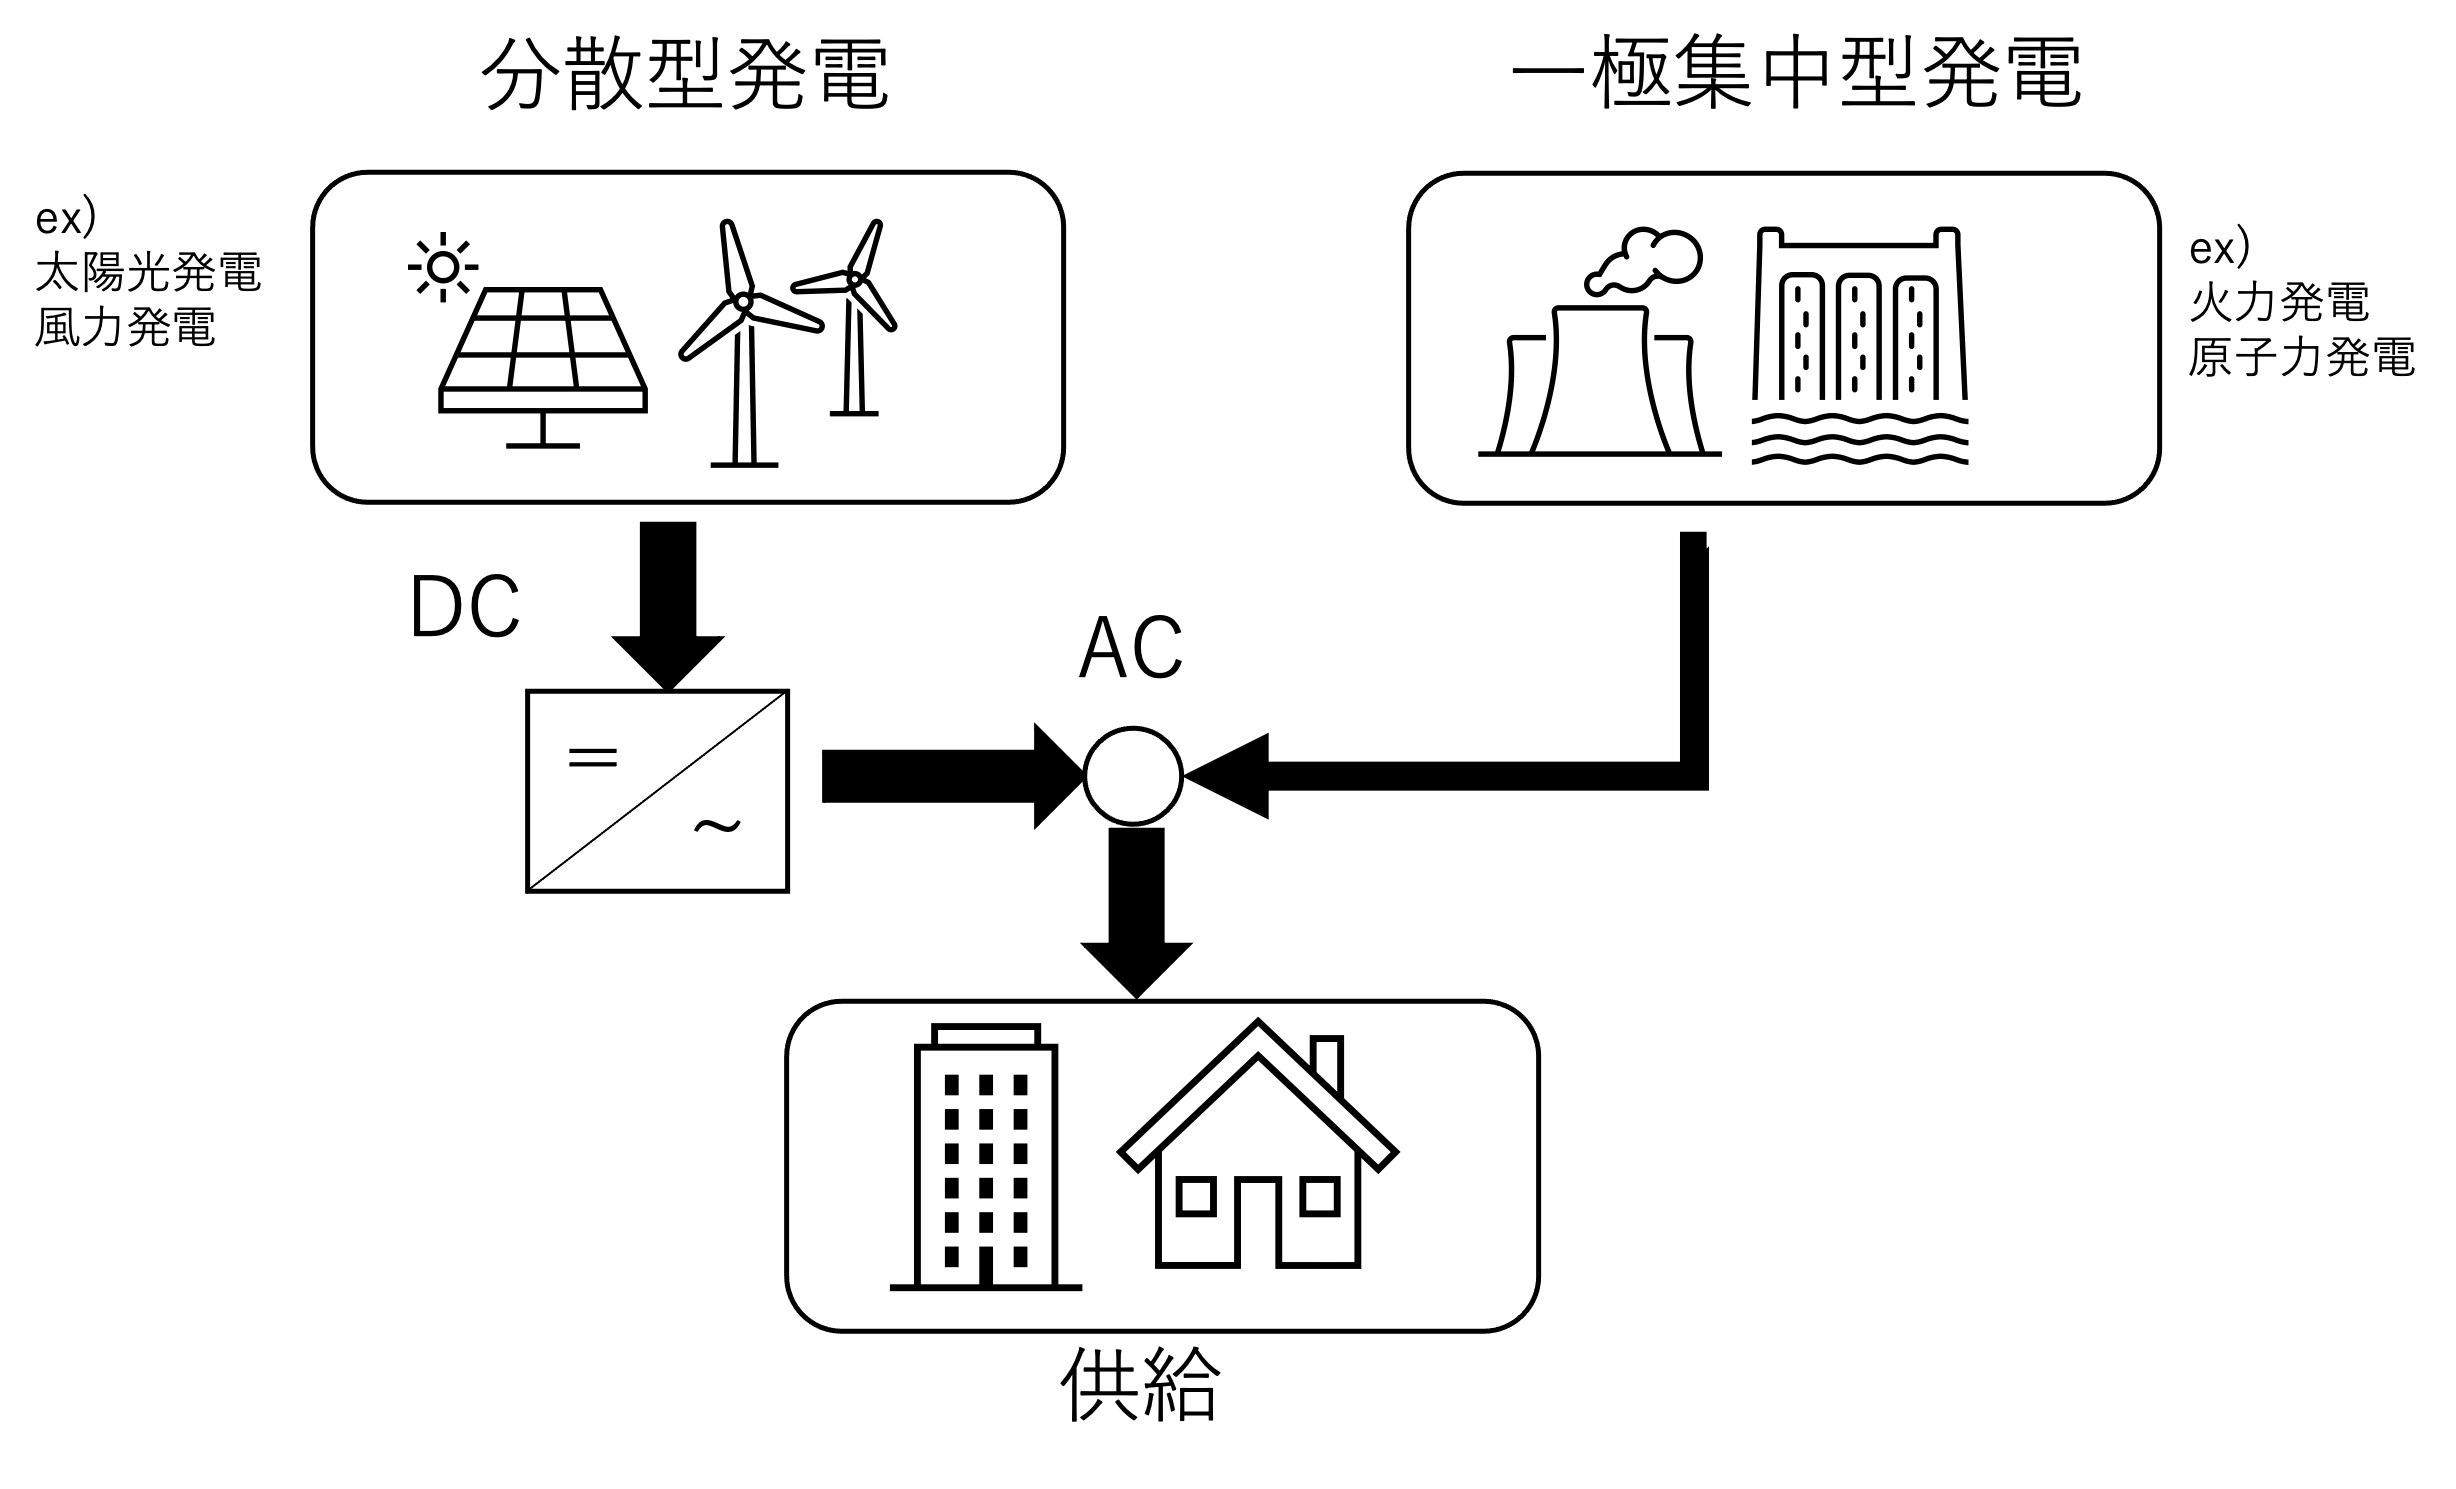
\includegraphics[width=140mm]{image/chapter1/Fig1.2.png}
    \caption{系統連系のイメージ図}
    \label{Fig1.2}
\end{figure}

現在では，分散型発電システムの需要拡大の観点から大容量な分散型発電システムの利用が進んでいる.電力容量が大容量になるにつれて接続される商用系統が高圧となり，従来のように系統電圧の情報をセンサで取得する場合，高価なセンサが必要となることや配線が複雑となるという問題がある.また，研究対象となる大規模太陽光発電システムについて，製品として提供しているものに連系リアクトル相当の配電盤は含まれておらず，配電盤は各需要家に存在するものであるため，連系リアクトルの値にばらつきが生じ，かつ系統電圧の情報をセンサから取得することが困難である.このことから，先行研究では大規模太陽光発電システムについて，連系リアクトルの値に依存しない制御手法の研究を行っていた．

\subsection{系統連系規定}
図\ref{Fig1.3}にFRT要件の一部事例を示す．
系統連系システムでは，分散型電源システム側で広範囲の瞬時電圧の低下や大規模電源脱落，周波数変動が発生した場合においても継続運転が可能となるために事故時運転継続要件(FRT:Fault Ride Through)を満たすシステムであることが求められている．この規定は日本電気技術企画委員会(JESC:Japan)により制定されている．

\newpage
\begin{figure}[ht]
    \center
    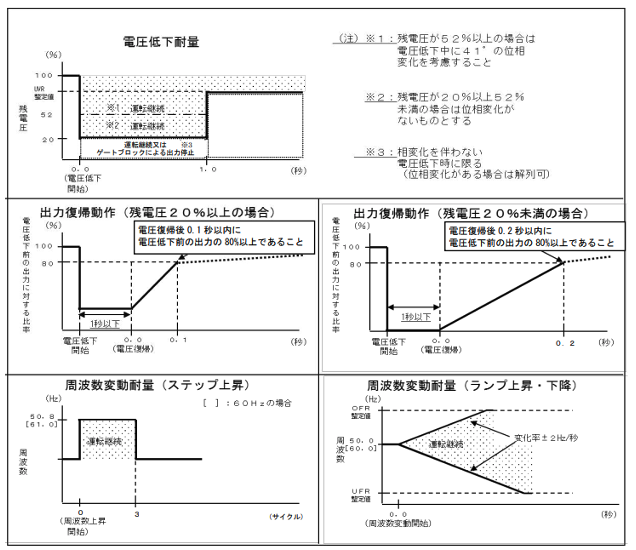
\includegraphics[width=140mm]{image/chapter1/Fig1.3.png}
    \caption{FRT要件の一部事例}
    \label{Fig1.3}
\end{figure}

FRT要件では，系統事故が発生し，系統電圧が20\%以下まで低下してもパワーコンディショナーのインバータを継続運転させて電力を供給する必要があり，系統電圧の低下立によって系統電圧復帰後にインバータの出力を80\%以上に戻すための許容時間が異なる．系統送電事故による広範囲の瞬時電圧低下・瞬時周波数上昇，大規模電源脱落，系統分離による周波数分離により，一斉解列や出力低下継続などが発生した場合，系統全体の電圧，周波数維持に大きな悪影響を及ぼす可能性があるため，パワーコンディショナーには事故発生時にも継続運転可能な高い制御性能が求められる．


%\newpage
\section{研究目的}
当研究室では，三角関数の積差の公式を用いて直交座標変換を行い，位相，振幅を算出する疑似dq変換を用いたPLL制御を提案している．
疑似dq変換はサンプリング周波数が高くなるとノイズの影響を受けやすくなり，検出精度が悪化してしまう．
これに対し，サンプリング周波数の異なる疑似dq変換回路を3並列化することでノイズの影響を低減している．
本研究では，ノイズ成分が相互に低減されるサンプリング周波数の組み合わせを探索し，
PLL制御の制御特性の向上を目的とする．\\
　疑似dq変換は系統電圧に対しての近似微分であるため，系統に低次高調波が含まれた場合に大きく動脈
してしまう．この課題に対し，複素係数フィルタを用いて系統電圧の瞬時複素ベクトルを容易
に算出し，なおかつ，優れた高調波外乱に対する耐性を有したPLL制御が提案されている\cite{ref03}．
複素係数フィルタを用いたPLL制御の初期検討として，複素係数フィルタの制御特性について検証する．
%Root main.tex
%---------------------------------------------------------------------------
%第2章　aaa
%---------------------------------------------------------------------------

\chapter{制御理論}
\label{chap:MotorDriveSystem}

\section{系統連系システム}
図(\ref{Fig2.1})に連系リアクトルなし三相系統連系システムの主回路図を示す．本システムは，T-NPC型三相系統連系インバータである．

\begin{figure}[ht]
    \center
    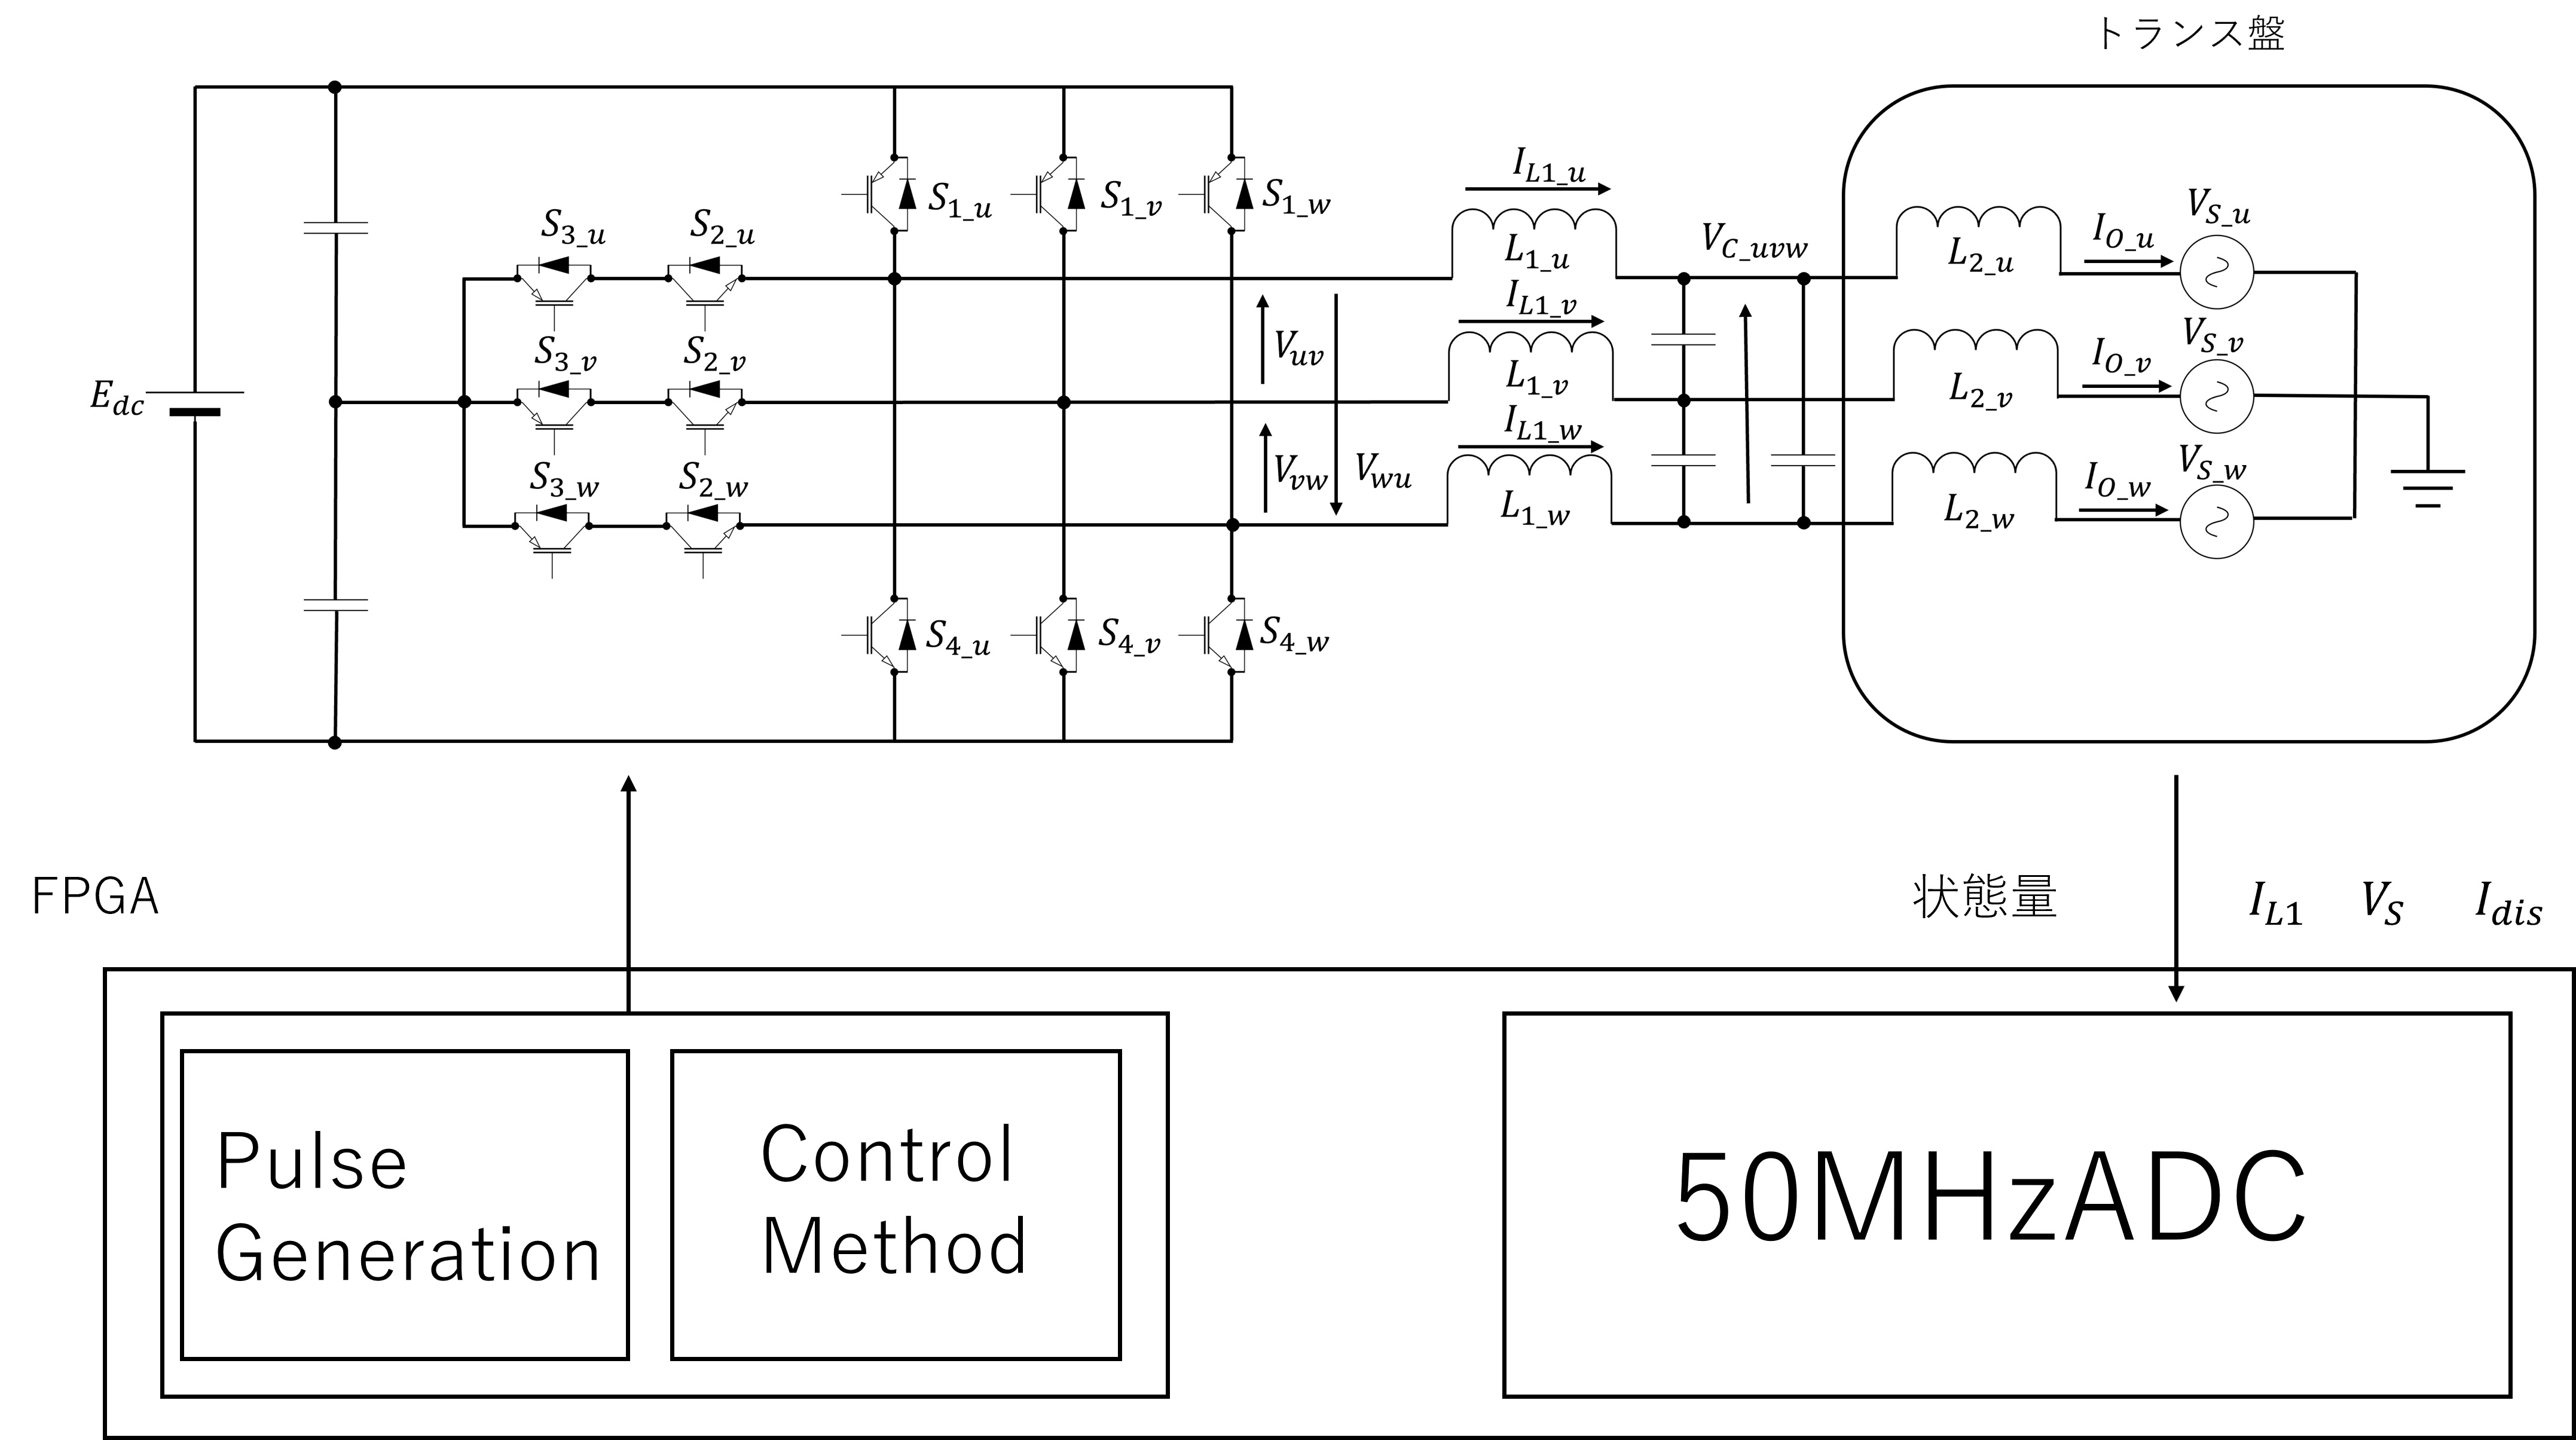
\includegraphics[width=140mm]{image/chapter2/fig.1.png}
    \caption{連系リアクトルなし三相系統連系システムの主回路図}
    \label{Fig2.1}
\end{figure}

%本システムは，分散型電源$E_{dc}$から供給される直流電圧をT-NPC型三相系統連系インバータで$0\si{V}$，\\$\pm $ $E_{dc}\si{V}$の矩形波電圧へ変換する．次にインダクタ$L_{1}$，コンデンサ$C$から構成される$LC$フィルタによって平滑化を行い，交流電圧(インバータ出力電圧)に変換し，連系リアクトル$L_{2}$を介して系統に接続する．また，インバータから連系リアクトル$L_{2}$を通して系統に流れる出力電流$I_{o}$はインバータ出力電圧$V_{c}$と系統電圧$V_{s}$間の電位差及び連系リアクトル$L_{2}$の容量に依存して流れる．

先行研究においては，連系リアクトル$L_{2}$に流れる出力電流$I_{o}$を制御対象としていたが，本研究では，連系リアクトルを制御対象に含まないため，フィルタインダクタ$L_{1}$に流れる電流$IL_{1}$を制御対象とする．

\section{三相二相変換・二相三相変換}
図\ref{Fig2.2}に三相交流のベクトルと二相交流のベクトルの関係図を示す．
本研究では，三相系統連系システムを制御対象として制御を行う．三相のシステムは，単相のシステムと異なり，各相の和が0となる三相平衡の性質から各相を独立して制御することが困難である．そのため，三相二相変換及び，二相三相変換を利用することで三相システムを2つの独立した単相システムとして制御することができる．

\begin{figure}[ht]
    \center
    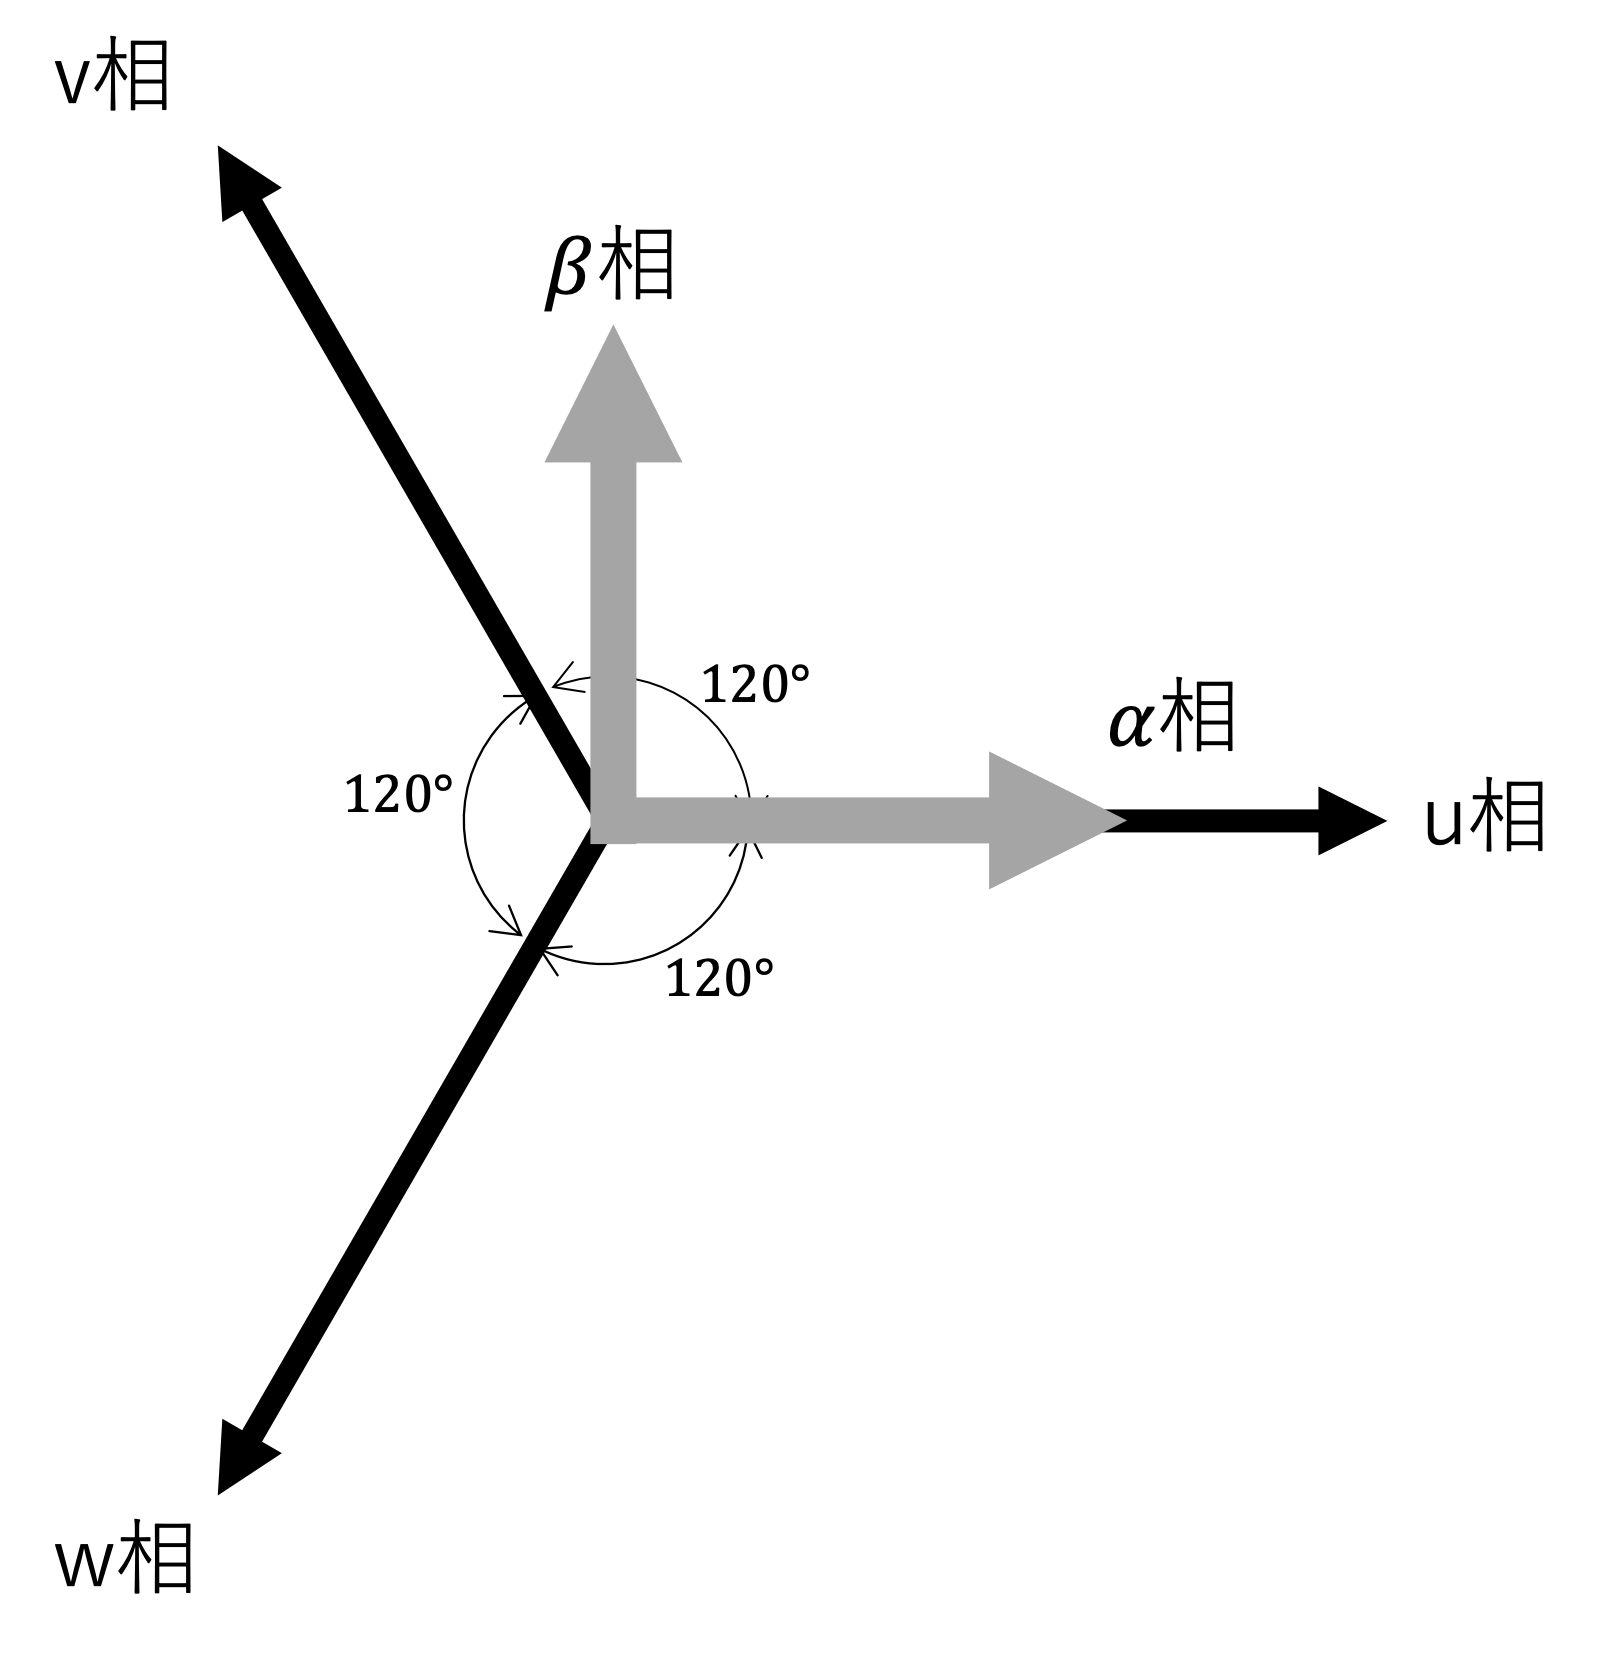
\includegraphics[width=60mm]{image/chapter2/Fig2.2.png}
    \caption{三相交流のベクトルと二相交流のベクトルの関係図}
    \label{Fig2.2}
\end{figure}

図\ref{Fig2.3}に三相二相変換・二相三相変換結果を示す．
三相二相変換とは，三相平衡によって振幅が等しく，隣り合う相の位相が$\frac{2\pi}{3}$だけずれた三相分の交流ベクトルを互いに直交な$\alpha$相と$\beta$相の軸へ成分分解する変換である\cite{3}．これにより三相交流ベクトルは互いに独立した$\alpha$相と$\beta$相のベクトルへ変換される．\par

\begin{figure}[ht]
    \center
    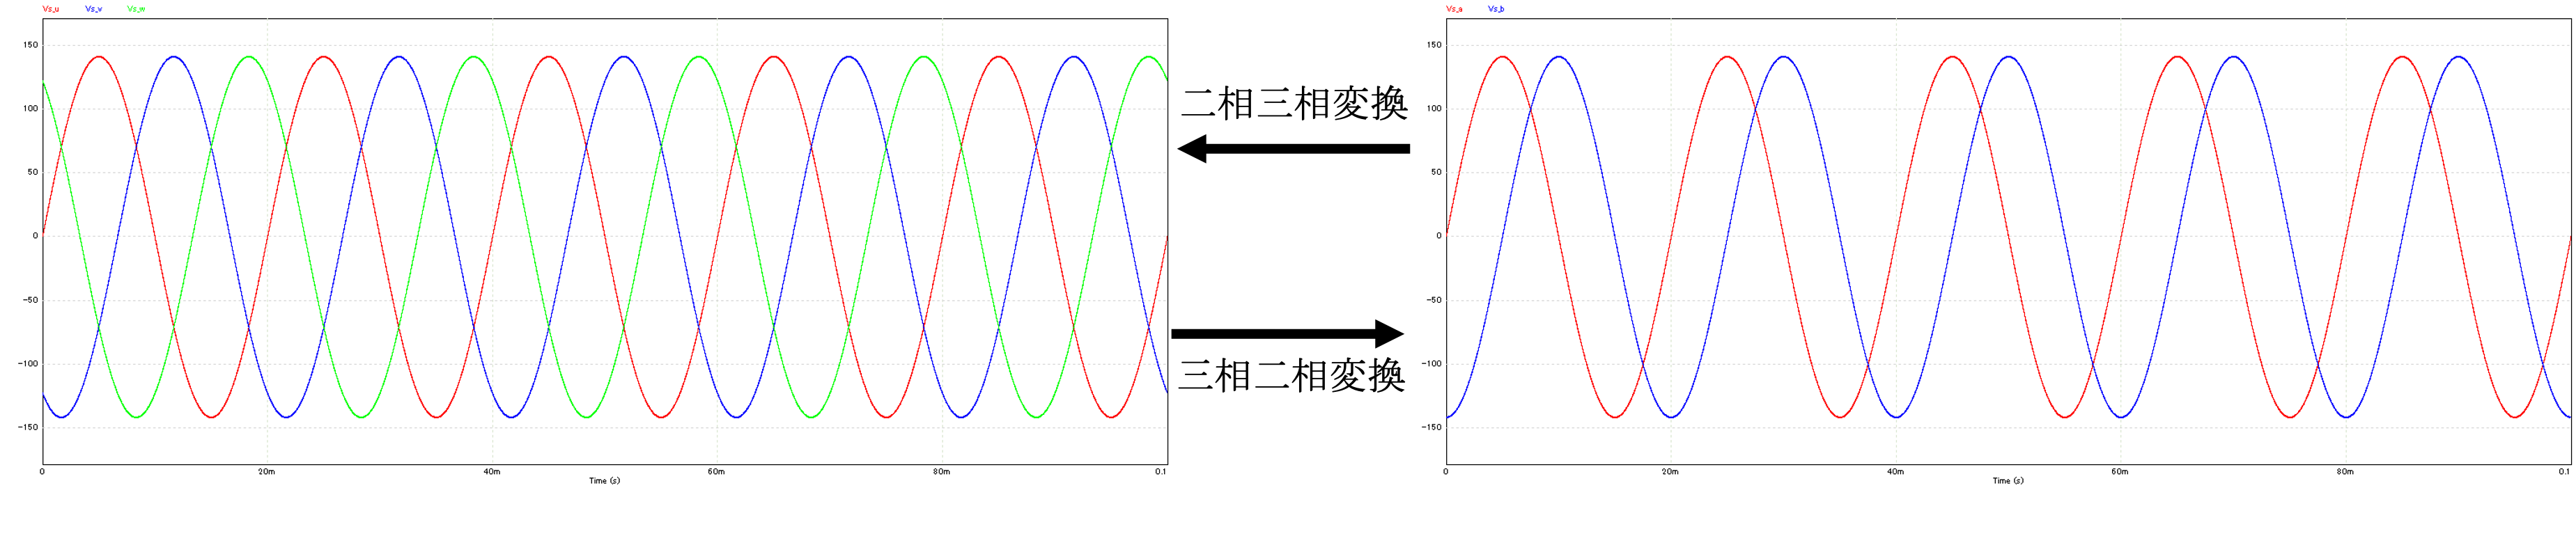
\includegraphics[width=140mm]{image/chapter2/Fig2.3.png}
    \caption{三相二相変換・二相三相変換結果}
    \label{Fig2.3}
\end{figure}

三相二相変換には，相対変換と絶対変換の2種類の方式がある．相対変換では三相と変換後の二相における正弦波の振幅が一致するが，二相における電力量が2/3倍となる．また，絶対変換では，三相と変換後の二相における正弦波の振幅は一致しないが，二相における電力量は一致する．本研究では相対変換を用いる．式(\ref{eq2.1})，(\ref{eq2.2})に三相二相(相間)相対変換，二相三相(相間)相対変換を示す．

\begin{equation}
    \begin{bmatrix}\label{eq2.1}
        x_{\alpha} \\ 
        x_{\beta}       
    \end{bmatrix}
    =\frac{2}{3}
    \begin{bmatrix}
        1 & -\frac{1}{2} & -\frac{1}{2} \\
        0 & -\frac{\sqrt{3}}{2} & -\frac{\sqrt{3}}{2}
    \end{bmatrix}
    \begin{bmatrix}
        x_{u}\\
        x_{v}\\
        x_{w}
    \end{bmatrix}
\end{equation}

\begin{equation}
    \begin{bmatrix} \label{eq2.2}
        x_{u}\\
        x_{v}\\
        x_{w}
    \end{bmatrix}
    =
    \begin{bmatrix}
        1 & 0\\
        -\frac{1}{2} & \frac{\sqrt{3}}{2}\\
        -\frac{1}{2} & -\frac{\sqrt{3}}{2}\\
    \end{bmatrix}
    \begin{bmatrix}
        x_{\alpha} \\
        x_{\beta}
    \end{bmatrix}
\end{equation}

式(\ref{eq2.3})，(\ref{eq2.4})に三相二相(相間)相対変換，二相三相(相間)相対変換を示す．
\begin{equation}
    \begin{bmatrix} \label{eq2.3}
        x_{\alpha} \\
        x_{\beta}
    \end{bmatrix}
    =\sqrt{\frac{2}{3}}
    \begin{bmatrix}
        1 & -\frac{1}{2} & -\frac{1}{2} \\
        0 & -\frac{\sqrt{3}}{2} & -\frac{\sqrt{3}}{2}
    \end{bmatrix}
    \begin{bmatrix}
        x_{u}\\
        x_{v}\\
        x_{w}
    \end{bmatrix}
\end{equation}

\begin{equation}
    \begin{bmatrix} \label{eq2.4}
        x_{u}\\
        x_{v}\\
        x_{w}
    \end{bmatrix}
    =\sqrt{\frac{2}{3}}
    \begin{bmatrix}
        1 & 0\\
        -\frac{1}{2} & \frac{\sqrt{3}}{2}\\
        -\frac{1}{2} & -\frac{\sqrt{3}}{2}\\
    \end{bmatrix}
    \begin{bmatrix}
        x_{\alpha} \\
        x_{\beta}
    \end{bmatrix}
\end{equation}

式(\ref{eq2.5})，(\ref{eq2.6})に三相二相(相間)相対変換，二相三相(相間)相対変換を示す．
\begin{equation}
    \begin{bmatrix} \label{eq2.5}
        x_{\alpha} \\
        x_{\beta}
    \end{bmatrix}
    =\frac{2}{3}
    \begin{bmatrix}
        \frac{1}{2} & 0 & -\frac{1}{2} \\
        0 & \frac{\sqrt{3}}{2} & 0
    \end{bmatrix}
    \begin{bmatrix}
        x_{uv}\\
        x_{vw}\\
        x_{wu}
    \end{bmatrix}
\end{equation}

\begin{equation}
    \begin{bmatrix} \label{eq2.6}
        x_{uv}\\
        x_{vw}\\
        x_{wu}
    \end{bmatrix}
    =\frac{3}{2}
    \begin{bmatrix}
        1  & -\frac{1}{\sqrt{3}}\\
        0  & \frac{2}{\sqrt{3}}\\
        -1 & -\frac{1}{\sqrt{3}}
    \end{bmatrix}
    \begin{bmatrix}
        x_{\alpha} \\
        x_{\beta}
    \end{bmatrix}
\end{equation}

\section{静止座標/回転座標の変換(dq変換)}
図\ref{Fig2.4}に静止座標系・回転座標系の関係図を示す．
静止座標系($\alpha-\beta$軸)上の変数($x_{\alpha}$，$x_{\beta}$)を角度$\theta$で回転する回転座標系($d-q$軸)の変数($x_{d}$，$x_{q}$)に変換する場合やその逆の変換を行うときに用いる制御測である．
\newpage

\begin{figure}[ht]
    \center
    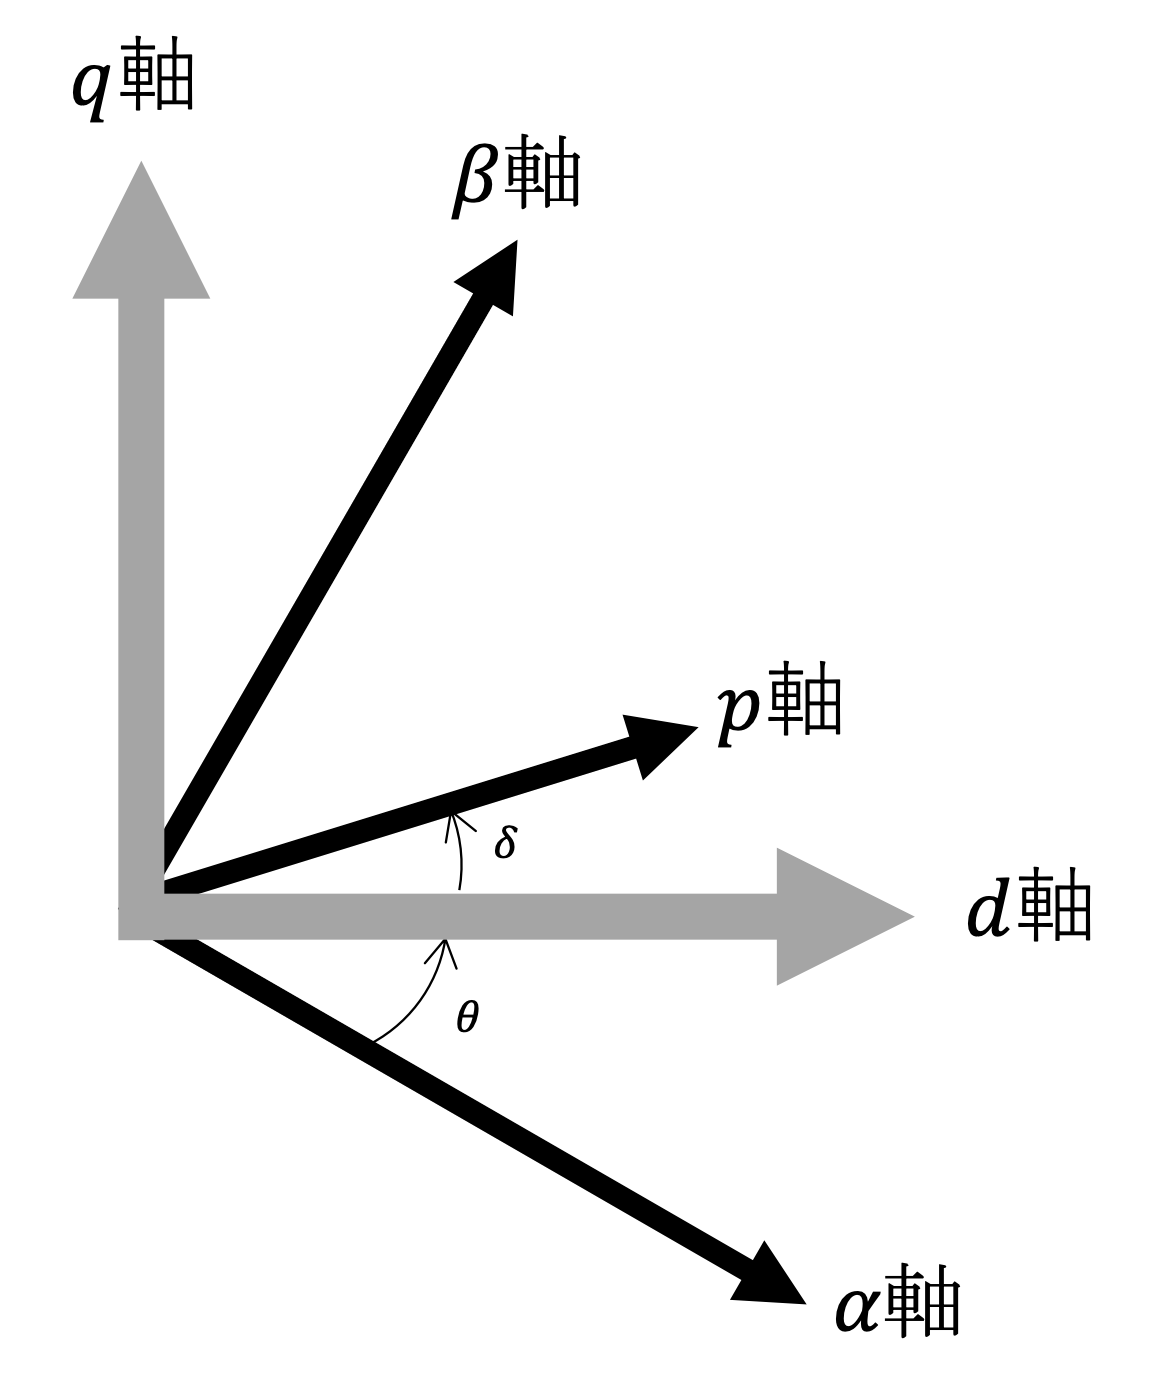
\includegraphics[width=60mm]{image/chapter2/Fig2.4.png}
    \caption{静止座標系・回転座標系の関係図}
    \label{Fig2.4}
\end{figure}

式(\ref{eq2.7})に静止座標系を回転座標系に変換する変換式を示す．
\begin{equation}
    \begin{bmatrix} \label{eq2.7}
        x_{d}\\
        x_{q}
    \end{bmatrix}
    =
    \begin{bmatrix}
        \cos{\theta} & \sin{\theta}\\
        -\sin{\theta}& \cos{\theta}
    \end{bmatrix}
    \begin{bmatrix}
        x_{\alpha} \\
        x_{\beta}
    \end{bmatrix}
\end{equation}

式(\ref{eq2.8})に回転座標系を静止座標系に変換する変換式を示す．
\begin{equation}
    \begin{bmatrix} \label{eq2.8}
        x_{\alpha}\\
        x_{\beta}
    \end{bmatrix}
    =
    \begin{bmatrix}
        \cos{\theta} & -\sin{\theta}\\
        -\sin{\theta}& \cos{\theta}
    \end{bmatrix}
    \begin{bmatrix}
        x_{d} \\
        x_{q}
    \end{bmatrix}
\end{equation}

図\ref{Fig2.5}にdq変換の結果を示す．

\begin{figure}[ht]
    \center
    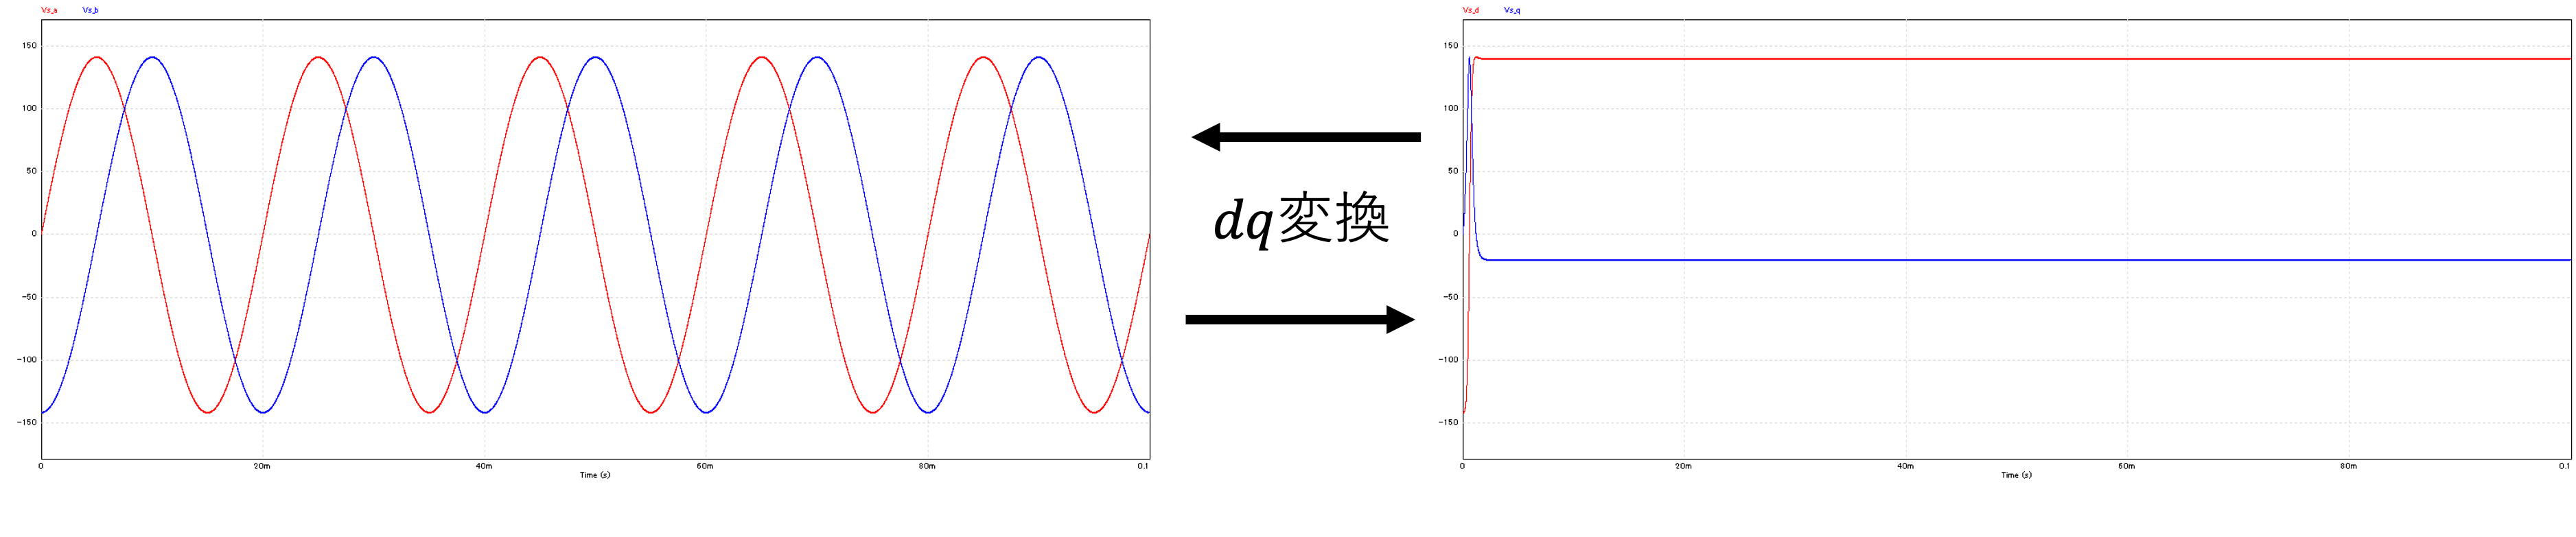
\includegraphics[width=140mm]{image/chapter2/Fig2.5.png}
    \caption{dq変換の結果}
    \label{Fig2.5}
\end{figure}

式(\ref{eq2.7})の様にdq変換を適用し，直交座標系に変換することで振幅相当である$x_{d}$，位相相当である$x_{q}$へ変換することができる．

\section{Phase-Locked-Loop(PLL)}
PLL制御は入力される周期的な信号をもとにフィードバック制御を行い，内部の信号を入力信号の周期に同期する制御である．図\ref{Fig2.6}にPLL制御フロー図を示す．
系統連系システムでは，出力電流を適切に制御するためにインバータの出力電圧の位相と系統電圧の位相を同期させることが必要となり，そのためにPhase-Locked-PLL(PLL)制御を適用する．

\begin{figure}[ht]
    \center
    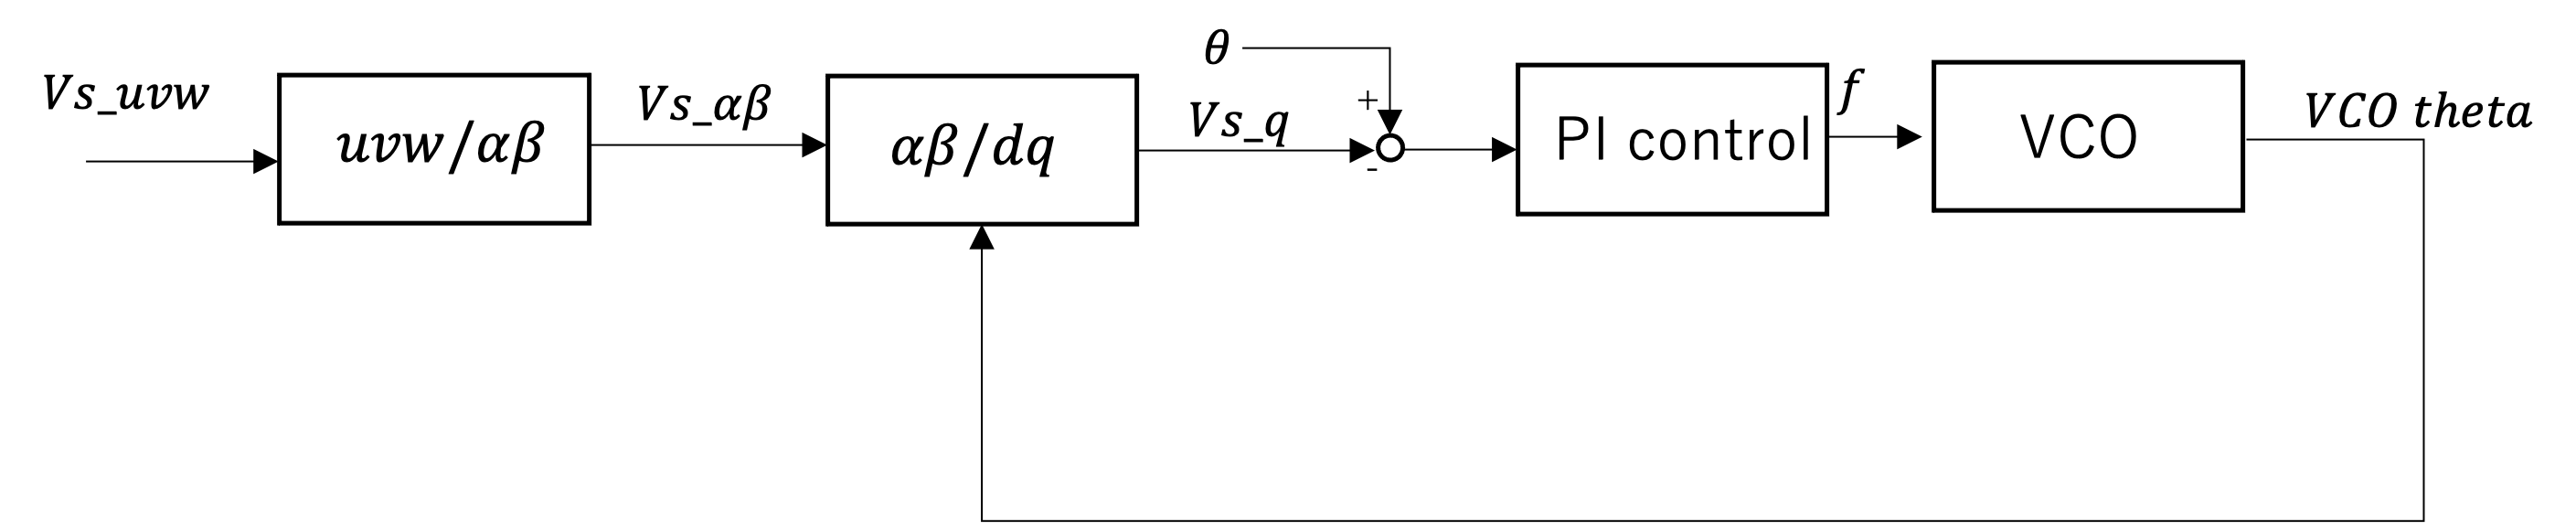
\includegraphics[width=140mm]{image/chapter2/Fig2.6_ver2.png}
    \caption{PLL制御フロー図}
    \label{Fig2.6}
\end{figure}

PLL制御では，系統電圧$V_{s}$に対して三相二相変換を適用することで直交座標系に変換する．その後dq変換を適用することで回転座標系を静止座標系に変換する．dq変換を適用することで振幅相当の$V_{sd}$，位相相当の$V_{sq}$に変換する．検出された位相差$V_{sq}$に対して位相差が0となるようにPI制御を行い，周波数を求める．導出した周波数からコントローラ内部の位相を生成するために，Voltage Controlled Oscillator(VCO)を適用する\cite{3}\cite{4}．


\section{シングルレートデッドビート制御}
デッドビート制御とは制御量を指令値に追従させるためのディジタル制御の一手法である．
図\ref{Fig2.7}に連系リアクトルなし三相系統連系システムの等価回路を示す．

\begin{figure}[ht]
    \center
    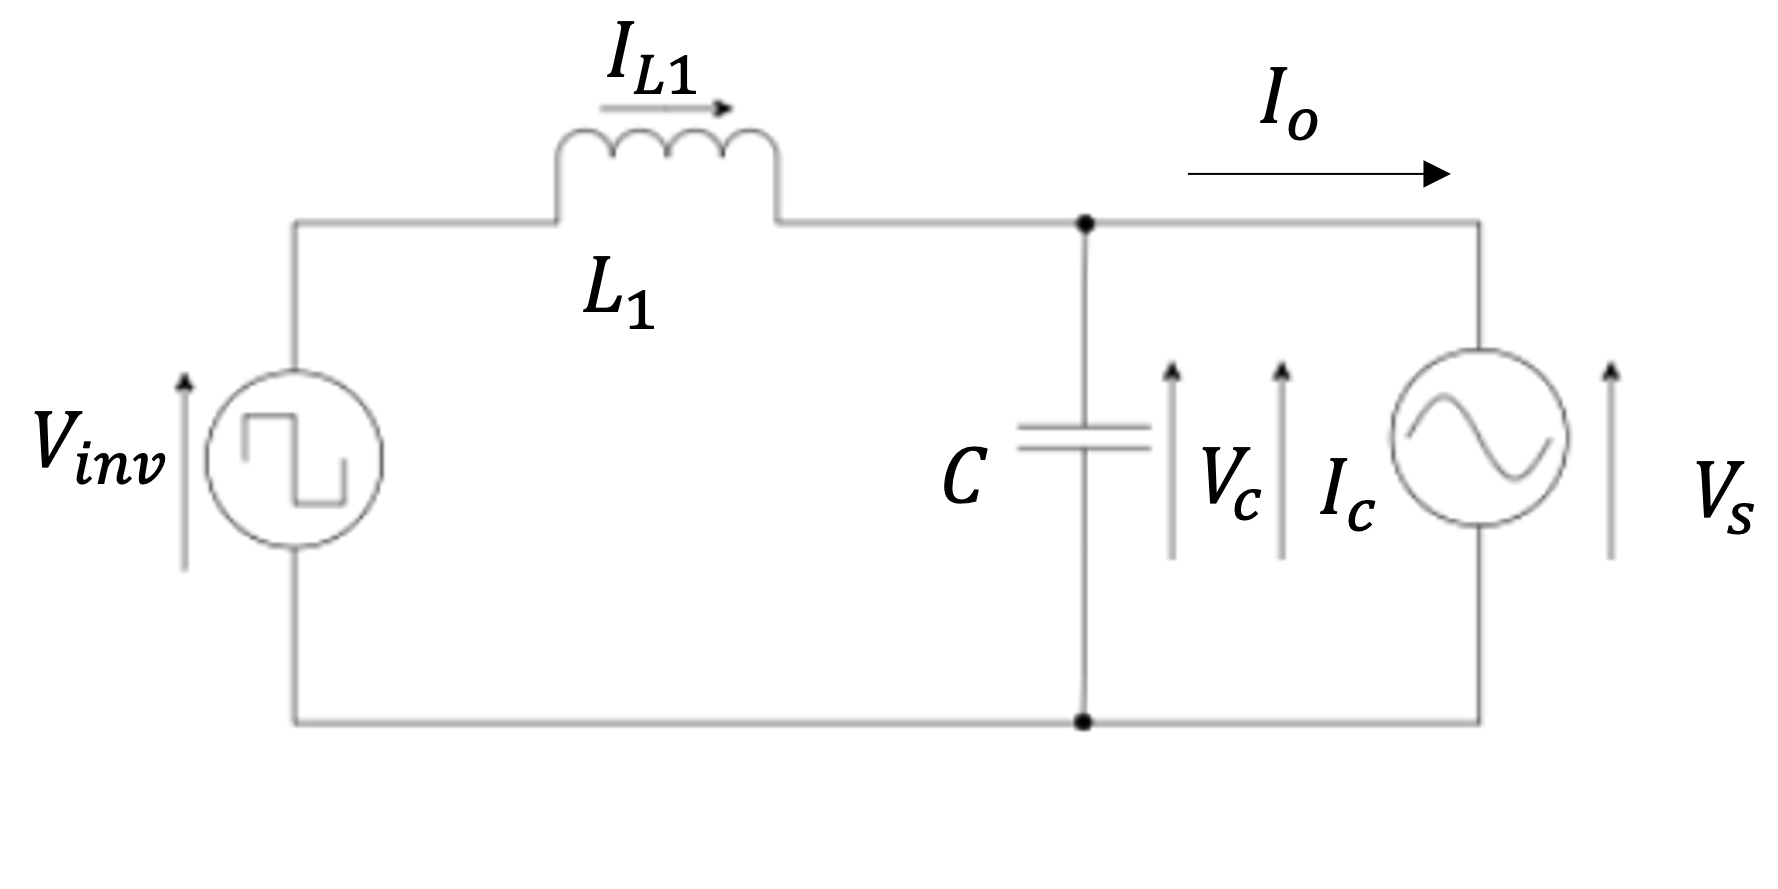
\includegraphics[width=110mm]{image/chapter2/Fig2.7.png}
    \caption{連系リアクトルなし三相系統連系システムの等価回路}
    \label{Fig2.7}
\end{figure}

デッドビート制御は，有限時間内に任意の状態変数を目標値に追従させるための制御であり，サンプリング点において制御量を指令値に追従させることができる．サンプリング点を$KT$，次のサンプリング点を$(K+1)T$としたとき，$(K+1)T$時点における制御量の値を指令値に追従させるために$KT$時点におけるシステムの各状態からインバータの出力電圧パルス指令値$\Delta T(K)$を求め，インバータの出力電圧パルス幅を$\Delta T(K)$とすることで$(K+1)T$時点において制御量を指令値と一致させる．\cite{4}\par
系統連系システムにおける連系インピーダンスの影響を無視した場合のノミナルモデルにおける連続時間状態方程式を示す．

\begin{align}
    &\dot{x}_{\alpha,\beta}=Ax_{\alpha,\beta}+Bu_{\alpha,\beta} \label{eq2.9}\\ &y=cx_{\alpha,\beta}              \label{eq2.10}
\end{align}

ただし式(1)について，

\begin{equation} 
    \begin{split}
       &x_{\alpha,\beta}=
    \begin{bmatrix} 
        I_{L1 \alpha,\beta}  \\
        V_{c\alpha,\beta}   \\
        I_{o\alpha,\beta}     \\
    \end{bmatrix}  \notag  
    ， A=
    \begin{bmatrix}     
        0           & -\frac{1}{L_{1}} &        0             \\
        \frac{1}{C} & 0                &     -\frac{1}{C}     \\ 
        0 & 0 & 0  \\
        0 & 0 & 0   \\
    \end{bmatrix}   \notag  
    &B=
    \begin{bmatrix}     
        \frac{1}{L_{1}}  \\
        0                \\
        0                \\
    \end{bmatrix}   \notag  
    ，u_{\alpha,\beta}=
    \begin{bmatrix}     
        V_{inv}    \\   
    \end{bmatrix}   \notag  
    \end{split}
\end{equation}

である．対象のモデルは連系リアクトル$L_2$を含まないモデルであり，本提案モデルでは，状態量として$I_{L1}$，$V_{c}$，$I_{dis}$，$I_{o}$を使用する．このとき，$I_{L1}$，$V_{c}$，$I_{dis}$の値はシステム上のセンサから取得するが，$I_o$は，センサから取得することができないことを想定しているため，コンデンサ電流$I_c$，インダクタ電流$IL_{1}$，を用いて数値計算を行い導出する．式(\ref{eq2.11})に出力電流の導出式を示す．

\begin{align}
    &I_{o \alpha,\beta}=I_{L1\alpha,\beta}-I_{c\alpha,\beta}   \label{eq2.11}    
\end{align}

式(\ref{eq2.9})の解は式(\ref{eq2.12})で表される．
\begin{align}
    x=e^{At}x(0)+\int_0^t e^{A(t-\tau)} Bu(\tau)d\tau  \label{eq2.12}
\end{align}

ただし，$x_{0}$は初期値である．図\ref{Fig2.8}に出力パルスのモデル図を示す．

\begin{figure}[ht]
    \center
    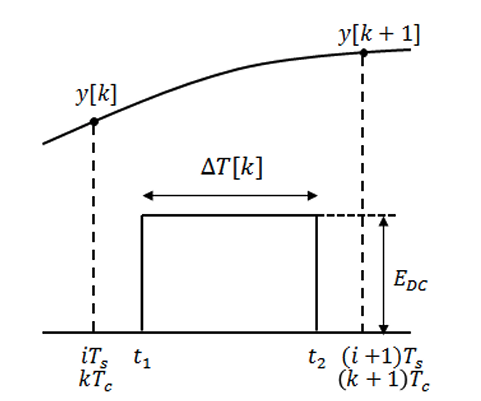
\includegraphics[width=80mm]{image/chapter2/Fig2.8.png}
    \caption{出力パルスのモデル図}
    \label{Fig2.8}
\end{figure}

入力$u$を幅が$\Delta T$のインバータの出力パルスとする．出力パルス$\Delta T$は図\ref{Fig2.8}のように1サンプル区間で左右対称で，大きさは電源電圧$\pm E_{dc}$，系統電圧$V_{s}$は1サンプリング区間において一定値であると仮定する．式(\ref{eq2.12})についてPWMホールドを適用すると，\par
$0\leq t< t_{1}$のときu=0より，式(\ref{eq2.12})は，
 
\begin{align}
    x(t_{1})=e^{A_{v}t}x(0)+\int_{0}^{t_{1}} e^{A(t-\tau)} Bu(\tau)d\tau \label{eq2.13}
\end{align}

$t_{1}\leq t< t_{2}$のときu=$\pm E_{dc}$，より，式(\ref{eq2.11})は，
 
\begin{equation}
    \begin{split}
        x(t_{2})&=e^{A(t_{2}-t_{1})}x(t_{1})+A^{-1}(e^{A(t_{2}-t_{1})}-I_{n})B(\pm E_{dc})+ \int_{t_{1}}^{t_{2}} e^{A(t-\tau)} Bu(\tau)d\tau  \\
        &=e^{A(t_{2}-t_{1})}x(t_{1})+A^{-1}(e^{A(\Delta T)}-I_{n})B(\pm E_{dc})+ \int_{0}^{t_{2}} e^{A(t-\tau)} Bu(\tau)d\tau    \label{eq2.14}
    \end{split}
\end{equation} 

$t_{2}\leq t< T_{s}$のときu=$0$，より，式(\ref{eq2.12})は，

\begin{equation}
    \begin{split}
        x(T_{s})=&e^{A(T_{s}-t_{2})}x(t_{2})+ \int_{t_{2}}^{T_{s}} e^{A(t-\tau)} Bu(\tau)d\tau  \\
        =&e^{A(T_{s}-t_{2})}{e^{A(t_{2})}x(0)+A^{-1}(e^{A(t_{2}-t_{1})}-I_{n})(\pm E_{dc})}\\  
        &+\int_{t_{2}}^{T_{s}} e^{A(t-\tau)} Bu(\tau)d\tau  \\
        =&e^{A(T_{s}}x(0)+e^{A(T_{s}-\Delta T)/2}A^{-1}(e^{A(\Delta T})-I_{n})B(\pm E_{dc})\\
        &+\int_{0}^{T_{s}} e^{A(t-\tau)} Bu(\tau)d\tau  \\ \label{eq2.15}
    \end{split}
\end{equation} 

ただし,
$\Delta T$は図\ref{Fig2.8}から$\Delta T=t_{2}-t_{1}$である．ここで，$e^{A\Delta T/2}$の2次のテイラー級数展開は以下の式で表される．

\begin{align}
    e^{A\Delta T/2} \approx 1+\frac{A\Delta T}{2}+\frac{A^2(\Delta T/2)^2}{2!} \label{eq2.16}
\end{align}

式(\ref{eq2.16})を式(\ref{eq2.15})に代入すると以下の式(\ref{eq2.17})が得られる．

\begin{align}
    x(T_{s})=e^{A(T_{s}}x(0)+e^{AT_{s}/2}A^{-1}B(\pm E_{dc})+\int_{0}^{T_{s}} e^{A(t-\tau)} Bu(\tau)d\tau  \label{eq2.17}
\end{align} 

以上のPWMホールドを用いて式(\ref{eq2.12})を離散化すると離散時間状態方程式は以下の式(\ref{eq2.18})のようになる\cite{5}．

\begin{align}
    x[k+1]=Fx[k]+G\Delta T[k] \label{eq2.18}
\end{align}

式(\ref{eq2.18})について，

\begin{equation} 
    \begin{split}
        F&=e^{ATs}   \\
        &=
    \begin{bmatrix} 
        F_{11} & F_{12} & F_{13}\\
        F_{21} & F_{22} & F_{23}\\
        F_{31} & F_{32} & F_{33}\\
    \end{bmatrix}  \notag  \\
        G&=e^{\frac{ATs}{2}}B(\pm E_{dc})   \\ 
        &=
    \begin{bmatrix}     
        g_{11}  \\
        g_{21}  \\
        g_{31}  \\
    \end{bmatrix}   \notag  \\ 
    \end{split}
\end{equation}

である．　ただし，$F$，$G$の各要素をそれぞれ$F_{ij}$，$G_{ij}$と表現する．$i,j$はそれぞれ第$i$行，第$j$列を意味する．
%各パルス指令信号は式(\ref{eq2.18})の$\Delata T[k]$について解くことで導出することができる．$\alpha $相，$\beta $相，の各パルス指令信号$\Delta T_{\alpha } [k]$，$\Delta T_{\beta }[k]$は，式(\ref{eq2.19})，(\ref{eq2.20})のように表すことができる．

\begin{equation}
    \begin{split}
        \Delta T_{\alpha [k]}=&\frac{I_{L\alpha}[k+1]-z11 I_{L1\alpha}[k]-z12 V_{c\alpha}[k]-z_{13} I_{o\alpha}[k]}{g11}  \label{eq2.19}
    \end{split}
\end{equation}

\begin{equation}
    \begin{split}
        \Delta T_{\beta [k]}=&\frac{I_{L\beta}[k+1]-z11 I_{L1\beta}[k]-z12 V_{c\beta}[k]-z_{13} I_{o\beta}[k]}{g11}    \label{eq2.20}
    \end{split}
\end{equation}

式(\ref{eq2.19})，(\ref{eq2.20})の様に導出された$\alpha$相と$\beta$相の操作量に対して二相三相変換することでU相，V相，W相の操作量を生成する．その後，導出した各相の操作量と三角波を比較するPWM制御を適用することでインバータのゲート信号を生成する．

\section{外乱補償型シングルレートデッドビート制御}
図\ref{Fig2.9}に外乱成分を追加した連系リアクトルなし三相系統連系システムの等価回路を示す．外乱補償型シングルレートデッドビート制御とは，シングルレートデッドビート制御に外乱成分を補償するための項を追加した制御である．先行研究では，外乱補償型シングルレートデッドビート制御を用いることでパラメータ変動等によって制御対象が案ノミナルとなった場合に外乱成分を抑制することでシステムのロバスト性が向上することが判明している\cite{7}．

\newpage
\begin{figure}[ht]
    \center
    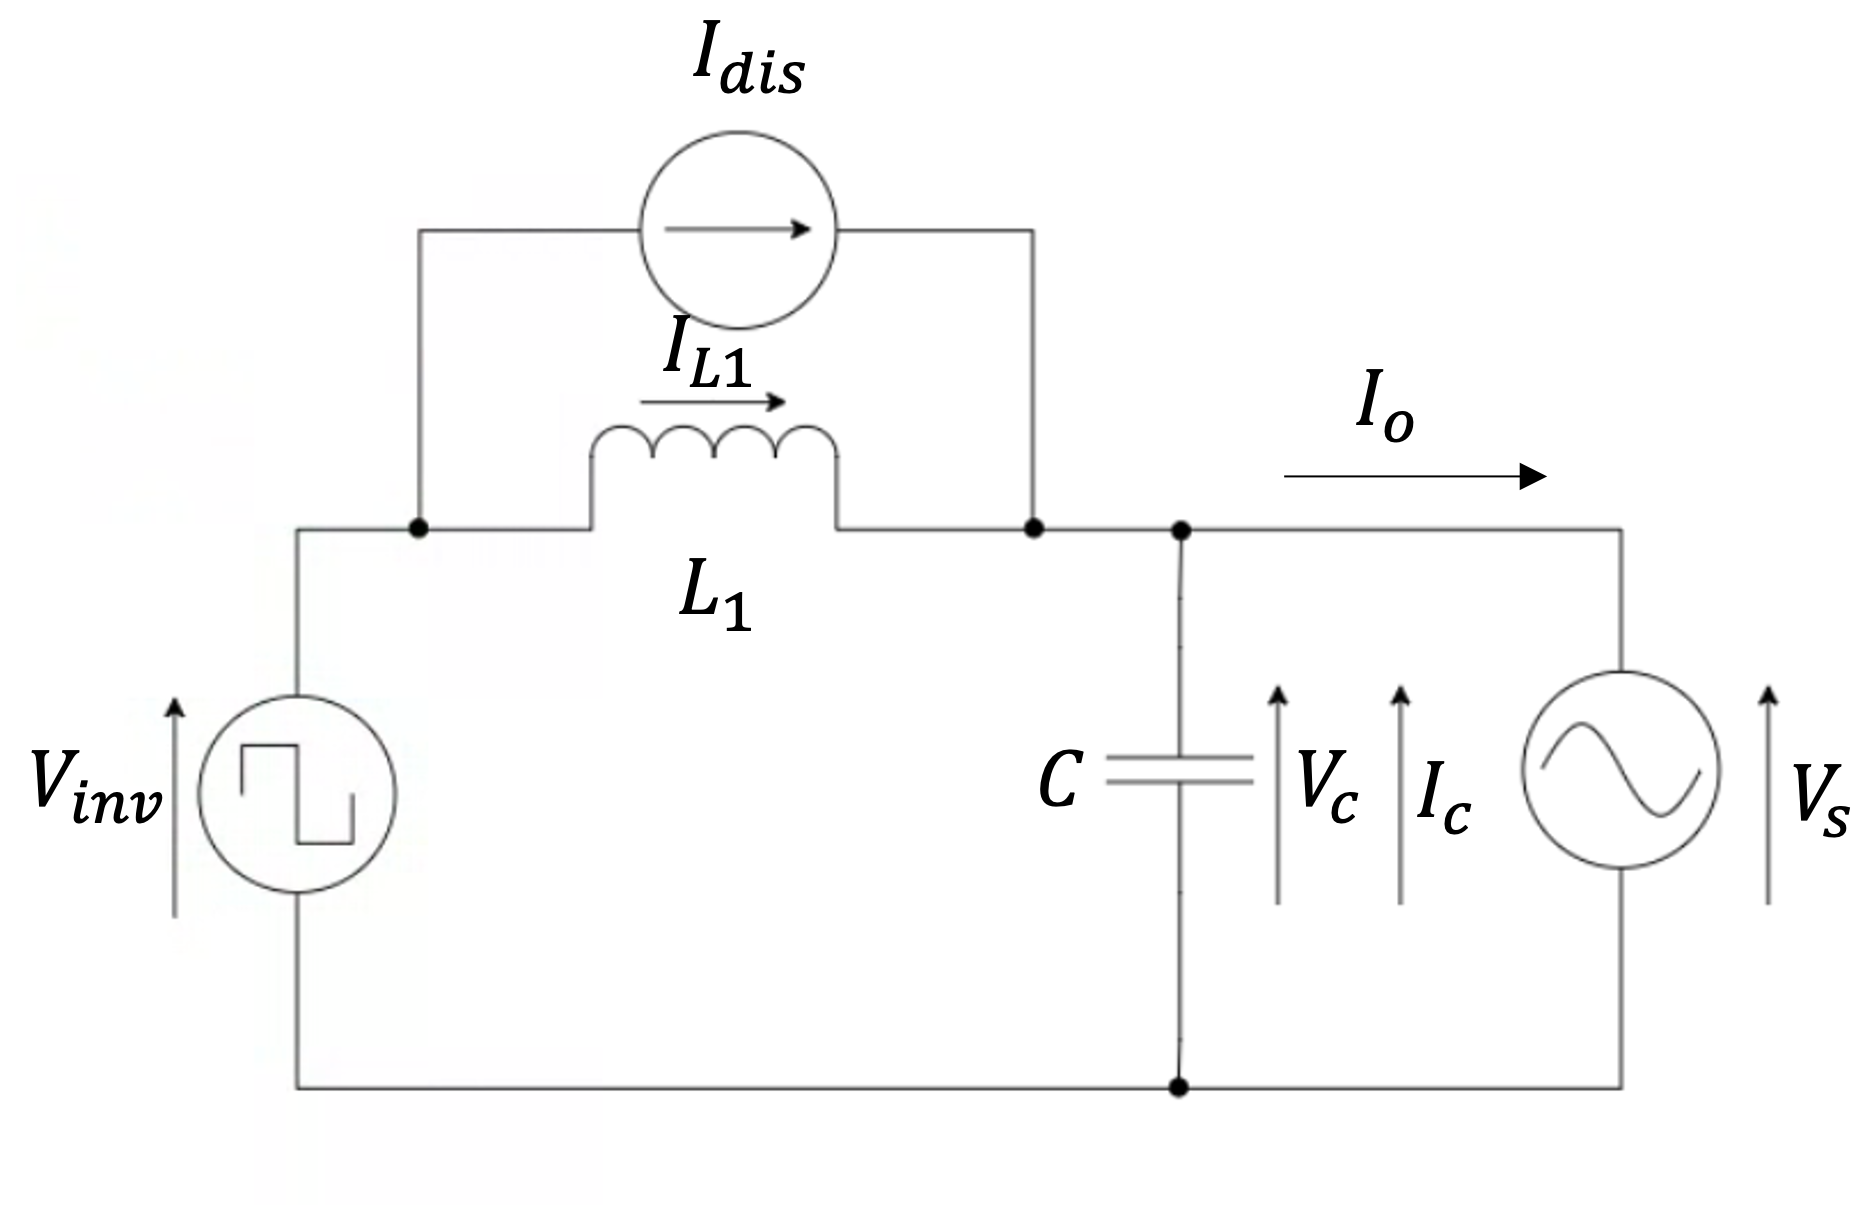
\includegraphics[width=80mm]{image/chapter2/Fig2.9.png}
    \caption{外乱成分を追加した連系リアクトルなし三相系統連系システムの等価回路}
    \label{Fig2.9}
\end{figure}

本研究において，外乱として想定するものは外乱電流であり，ノミナル時における出力電流以外を外乱電流とする．

\begin{align}
    &\dot{x}_{\alpha,\beta}=Ax_{\alpha,\beta}+Bu_{\alpha,\beta} \label{eq2.21}\\ &y=cx_{\alpha,\beta}              \label{eq2.22}
\end{align}

ただし式(\ref{eq2.21})について，

\begin{equation} 
    \begin{split}
       &x_{\alpha,\beta}=
    \begin{bmatrix} 
        I_{L1 \alpha,\beta}  \\
        V_{c\alpha,\beta}   \\
        I_{o\alpha,\beta}     \\
        I_{dis\alpha,\beta} \\
    \end{bmatrix}  \notag  
    ， A=
    \begin{bmatrix}     
        0           & -\frac{1}{L_{1}} &        0           & 0  \\
        \frac{1}{C} & 0                &     -\frac{1}{C}     &  \frac{1}{C} \\ 
        0 & 0 & 0 & 0  \\
        0 & 0 & 0 & 0  \\
    \end{bmatrix}   \notag  
    &B=
    \begin{bmatrix}     
        \frac{1}{L_{1}}  \\
        0                \\
        0                \\
        0                \\
    \end{bmatrix}   \notag  
    ，u_{\alpha,\beta}=
    \begin{bmatrix}     
        V_{inv}    \\   
    \end{bmatrix}   \notag  
    \end{split}
\end{equation}

である．対象のモデルは連系リアクトル$L_2$を含まないモデルであり，本モデルでは，状態量として$I_{L1}$，$V_{c}$，$I_{dis}$，$I_{o}$を使用する．このとき，$I_{L1}$，$V_{c}$，$I_{dis}$の値はシステム上のセンサから取得するが，$I_o$は，センサから取得することができないことを想定しているため，にコンデンサ電流$I_c$，インダクタ電流$IL_{1}$，外乱電流$I_{dis}$を用いて数値計算を行い導出する．式(\ref{eq2.23})に出力電流の導出式を示す．

\begin{align}
    &I_{o \alpha,\beta}=I_{L1\alpha,\beta}+I_{dis\alpha,\beta}-I_{c\alpha,\beta}   \label{eq2.23}    
\end{align}

式(\ref{eq2.21})の解は式(\ref{eq2.24})で表される．
\begin{align}
    x=e^{At}x(0)+\int_0^t e^{A(t-\tau)} Bu(\tau)d\tau  \label{eq2.24}
\end{align}

ただし，$x_{0}$は初期値である．入力$u$を幅が$\Delta T$のインバータの出力パルスとする．出力パルス$\Delta T$は図\ref{Fig2.8}のように1サンプル区間で左右対称で，大きさは電源電圧$\pm E_{dc}$，系統電圧$V_{s}$は1サンプリング区間において一定値であると仮定する．式(\ref{eq2.24})についてPWMホールドを適用すると\par
$0\leq t< t_{1}$のときu=0より，式(\ref{eq2.24})は，
 
\begin{align}
    x(t_{1})=e^{A_{v}t}x(0)+\int_{0}^{t_{1}} e^{A(t-\tau)} BV_{s}(\tau)d\tau \label{eq2.25}
\end{align}

$t_{1}\leq t< t_{2}$のときu=$\pm E_{dc}$，より，式(\ref{eq2.24})は，
 
\begin{equation}
    \begin{split}
        x(t_{2})&=e^{A(t_{2}-t_{1})}x(t_{1})+A^{-1}(e^{A(t_{2}-t_{1})}-I_{n})B(\pm E_{dc})+ \int_{t_{1}}^{t_{2}} e^{A(t-\tau)} BV_{s}(\tau)d\tau  \\
        &=e^{A(t_{2}-t_{1})}x(t_{1})+A^{-1}(e^{A(\Delta T)}-I_{n})B(\pm E_{dc})+ \int_{0}^{t_{2}} e^{A(t-\tau)} BV_{s}(\tau)d\tau    \label{eq2.26}
    \end{split}
\end{equation} 

$t_{2}\leq t< T_{s}$のときu=$0$，より，式(\ref{eq2.24})は，

\begin{equation}
    \begin{split}
        x(T_{s})=&e^{A(T_{s}-t_{2})}x(t_{2})+ \int_{t_{2}}^{T_{s}} e^{A(t-\tau)} BV_{s}(\tau)d\tau  \\
        =&e^{A(T_{s}-t_{2})}{e^{A(t_{2})}x(0)+A^{-1}(e^{A(t_{2}-t_{1})}-I_{n})(\pm E_{dc})}\\  
        &+\int_{t_{2}}^{T_{s}} e^{A(t-\tau)} BV_{s}(\tau)d\tau  \\
        =&e^{A(T_{s}}x(0)+e^{A(T_{s}-\Delta T)/2}A^{-1}(e^{A(\Delta T})-I_{n})B(\pm E_{dc})\\
        &+\int_{0}^{T_{s}} e^{A(t-\tau)} BV_{s}(\tau)d\tau  \\ \label{eq2.27}
    \end{split}
\end{equation} 

式(\ref{eq2.17})を式(\ref{eq2.27})に代入すると以下の式(\ref{eq2.28})が得られる．

\begin{align}
    x(T_{s})=e^{A(T_{s}}x(0)+e^{AT_{s}/2}A^{-1}B(\pm E_{dc})+\int_{0}^{T_{s}} e^{A(t-\tau)} BV_{s}(\tau)d\tau   \label{eq2.28}
\end{align} 

以上のPWMホールドを用いて式(\ref{eq2.24})を離散化すると離散時間状態方程式は以下の式のようになる．

\begin{align}
    x[k+1]=Fx[k]+G\Delta T[k] \label{eq2.29}
\end{align}

式(\ref{eq2.29})について，

\begin{equation} 
    \begin{split}
        F&=e^{ATs}   \\
        &=
    \begin{bmatrix} 
        F_{11} & F_{12} & F_{13} & F_{14}\\
        F_{21} & F_{22} & F_{23} & F_{24}\\
        F_{31} & F_{32} & F_{33} & F_{34}\\
        F_{41} & F_{42} & F_{43} & F_{44}\\
    \end{bmatrix}  \notag  \\
        G&=e^{\frac{ATs}{2}}B(\pm E_{dc})   \\ 
        &=
    \begin{bmatrix}     
        g_{11}  \\
        g_{21}  \\
        g_{31}  \\
        g_{41}  \\
    \end{bmatrix}   \notag  \\ 
    \end{split}
\end{equation}

である．　ただし，$F$，$G$の各要素をそれぞれ$F_{ij}$，$G_{ij}$と表現する．$i,j$はそれぞれ第$i$行，第$j$列を意味する．
%各パルス指令信号は式(\ref{eq2.29})の$\Delata T[k]$について解くことで導出することができる．$\alpha $相，$\beta $相，の各パルス指令信号$\Delta T_{\alpha } [k]$，$\Delta T_{\beta }[k]$は，式(\ref{eq2.30})，(\ref{eq2.31})のように表すことができる．

\begin{equation}
    \begin{split}
        \Delta T_{\alpha [k]}=&\frac{I_{L\alpha}[k+1]-z11 I_{L1\alpha}[k]-z12 V_{c\alpha}[k]-z_{13} I_{o\alpha}[k]-z14 I_{dis\alpha}[k]}{g11}  \label{eq2.30}
    \end{split}
\end{equation}

\begin{equation}
    \begin{split}
        \Delta T_{\beta [k]}=&\frac{I_{L\beta}[k+1]-z11 I_{L1\beta}[k]-z12 V_{c\beta}[k]-z_{13} I_{o\beta}[k]-z14 I_{dis\beta}[k]}{g11}    \label{eq2.31}
    \end{split}
\end{equation}

式(\ref{eq2.30})，(\ref{eq2.31})の様に導出された$\alpha$相と$\beta$相の操作量に対して二相三相変換することでU相，V相，W相の操作量を生成する．その後，導出した各相の操作量と三角波を比較するPWM制御を適用することでインバータのゲート信号を生成する．

\section{インダクタ電流指令値生成}
本研究においてデッドビート制御における制御量はフィルタインダクタ$L_{1}$に流れる電流$I_{L1}$である．制御対象であるインダクタ電流の指令値$I_{L1 ref}$はノミナル電流の振幅$I_{nom amp}$，PLL制御によって導出した位相角VCOを用いて以下の式(\ref{eq2.32})で表される．
\begin{align}
    I_{L1 ref}=I_{nom amp}\times \sin(VCO) \label{eq2.32}
\end{align}

式(\ref{eq2.32})では，PLL制御によって導出された系統電圧のU相の位相に同期した位相角を元に指令値の生成を行なっている．

\section{マルチサンプリングデッドビート制御}
図\ref{Fig2.10}にマルチサンプリング制御のイメージ図を示す．

\newpage

\begin{figure}[ht]
    \center
    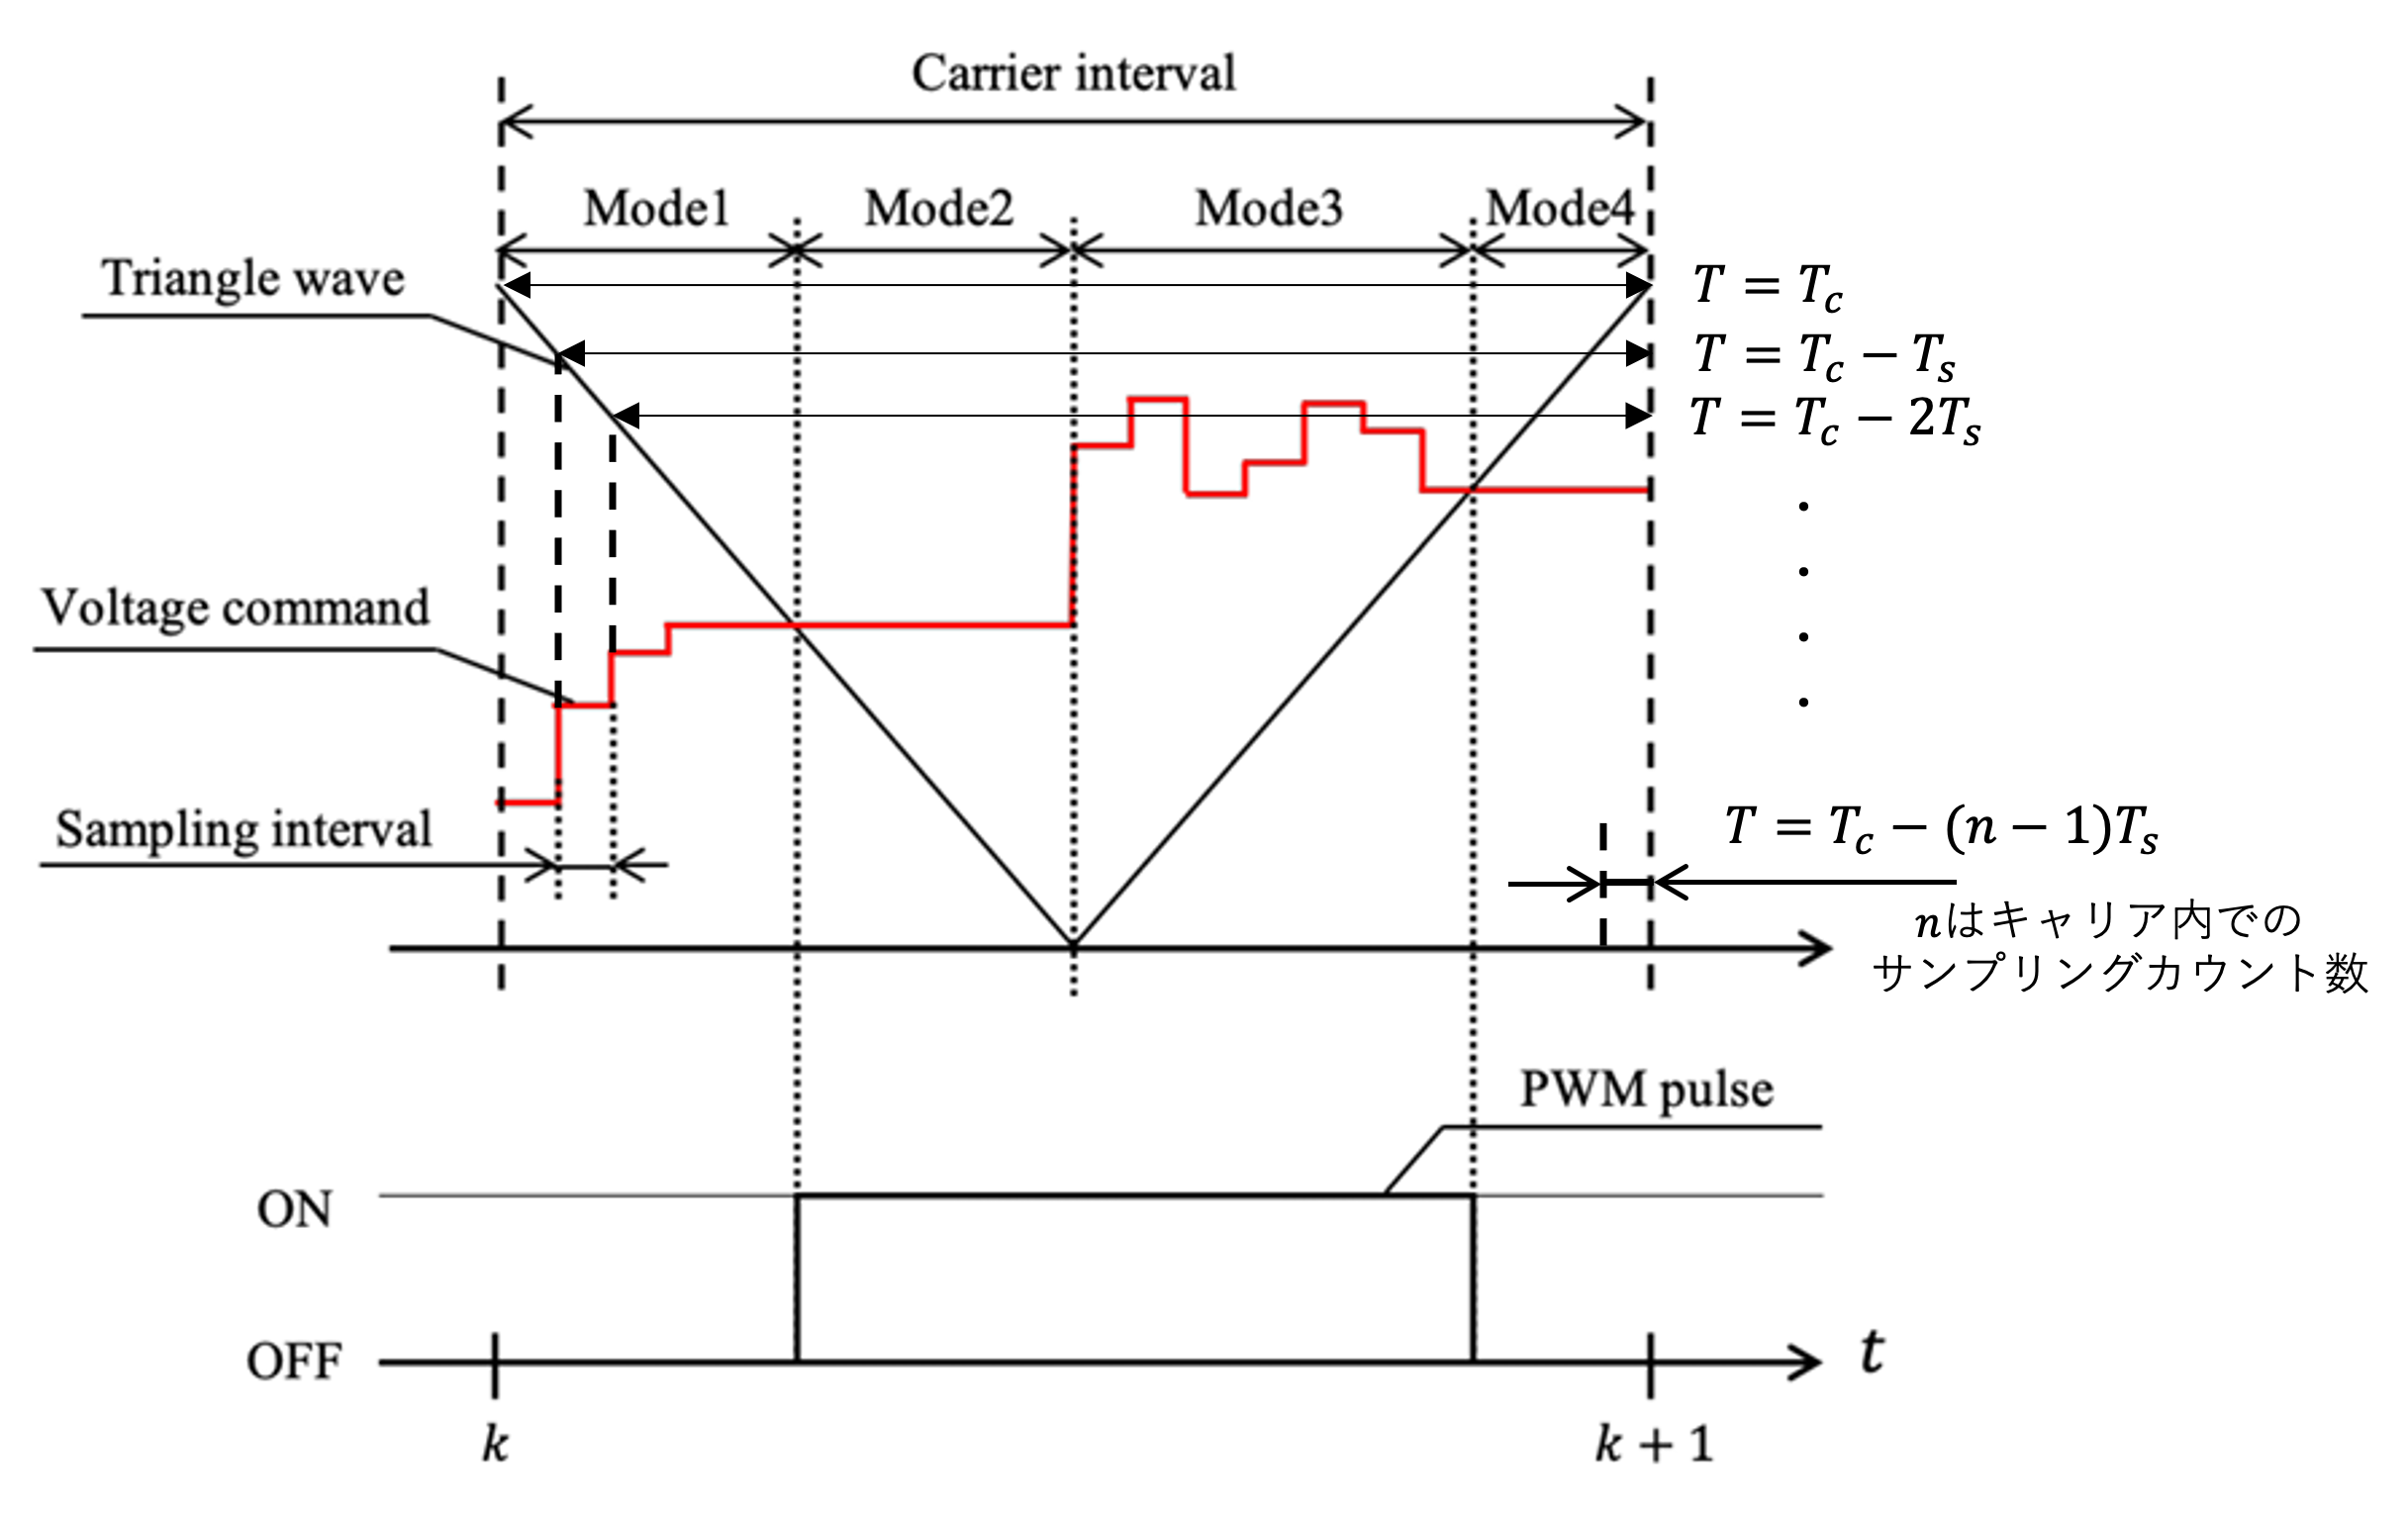
\includegraphics[width=110mm]{image/chapter2/Fig2.10.png}
    \caption{マルチサンプリング制御のイメージ図}
    \label{Fig2.10}
\end{figure}

マルチサンプリングデッドビート制御とは，キャリア周期$T_{c}$に対してでサンプリング周期$T_{s}$を小さくすることでとパルス指令の演算を複数回行うマルチサンプリング手法をデッドビート制御に適用したものである\cite{8}．\par
マルチサンプリングデッドビート制御では，PWMパルスの二度切りを防止するために動作モードが４つに分かれている．それぞれをmode1，mode2,mode3,mode4としている．以下に各モードの説明を示す．\\
\\
mode1：パルスのONタイミングを決定するmodeであり，1サンプリング毎にパルス指令値の演算を行い，三角波と等しくなった点をON時間とする．\\
\\
mode2：パルスがOFFになることを防ぐためのmodeであり，mode1の三角波とパルス指令値が等しくなった点からキャリア周期の半分までmode1の出力を保持する．\\
\\
mode3:パルスのOFFタイミングを決定するmodeであり，1サンプリング毎にパルス指令値の演算を行い，三角波と等しくなった点をOFF時間とする．\\
\\
mode4：パルスがONになることを防ぐためのmodeであり，mode3の三角波とパルス指令値が等しくなった点から次の周期の開始までmode3の出力を保持する．\\
%Root main.tex
%---------------------------------------------------------------------------
%第2章　aaa
%---------------------------------------------------------------------------

\chapter{シミュレーション}
\label{chap:シミュレーション}

\section{シミュレーション}
本シミュレーションでは，連系リアクトルなし3相系統連系システムにおいて，定常運転時，系統擾乱発生時及び，アンノミナル時の出力応答の確認を行う．制御手法として，外乱補償型シングルレートデッドビート制御，外乱補償型マルチサンプリングデッドビート制御を適用する．本シミュレーションでは，系統電圧実行時が系統擾乱によって80\%瞬時低下する場合を想定し，インダクタ電流$I_{L1}$の応答を確認する．回路シミュレータはPSIMを用いた．本シミュレーションのパラメータを表\ref{Tab3.1}に示す．

\begin{table}[ht]
    \centering
    \caption{系統連系システムのパラメータ}
    \begin{tabular}{c|c|c}\hline\hline
         Condition          &Parameter  &Value\\ \hline
         Sampling frequency & $f_{s}$[kHz]   & 100 \\
         Carrier frequency  & $f_{c}$[kHz]   & 100 \\
         Nominal capacity   & $P$[MVA]       & 1.0 \\
%         Grid Voltage       & $V_{s}$[V_{rms}]   & 400 \\
         Operating frequency& $f$[Hz]       & 50 \\
         Dc power supply    & $E_{dc}$[V]  & 1200 \\
%         Filter inductor    & $L_{1}$[$\si{\mu }$H]   & 51 \\
%         Filter capacitor   & $C$[$\si{\mu }$F]       & 995 \\
%         Interconnection inductor & $L2$[$\si{\mu }$H] & 51 \\ \hline
    \end{tabular}
    \label{Tab3.1}
\end{table}

評価指標として，定常運転時の出力電流 Il1 の全高調波歪成分 [\%](THD:Total Har-monic Distriction) に関して評価を行った.  全高調波歪成分は，値が低ければ高調波成分の含有率が低く波形の精度が高いと評価できる．\par

 THDを求めるための式を以下に示す．なお，$I_{L1}$は基本波の実効値，$I_{L1n}$はn次高調波の実行値を表す．
\begin{align}
    THD=\frac{\sqrt{\sum_{n-2}^{\infty}-I^2_{L1n}}}{I_{L1}} \label{eq8}
\end{align}

FRT要件よりTHDは5.0\%以下が運転条件となっている．
表\ref{Tab3.2}にアンノミナル条件時のパラメータを示す．
\begin{table}[htb]
\centering
  \caption{パラーメータの変更パターン}
  \begin{tabular}{c|c|c|c}  \hline\hline 
    \multirow{2}{*}{Condition}& \multicolumn{3}{|c}{Parameter} \\  \cline{2-4}
     & $L_{1}$ & $C$  & $L_{2}$\\  \hline 
%    ノミナル時 & $51 \si{\mu }$H & $995 \si{\mu }$F & $51 \si{\mu }$H \\ 
    パターン1 & 1.5 mH & 2.0 mF & 0.2 mH \\ 
    パターン2 & 0.35 mH & 200 $\mu $F & 0.002 mH\\ \hline
  \end{tabular}
  \label{Tab3.2}
\end{table}

\section{シミュレーション結果}
\subsection{ノミナル検証}
外乱補償型シングルレートデッドビート制御の際の定常運転時と系統擾乱発生時の出力応答を示す．

\begin{figure}[ht]
    \center
    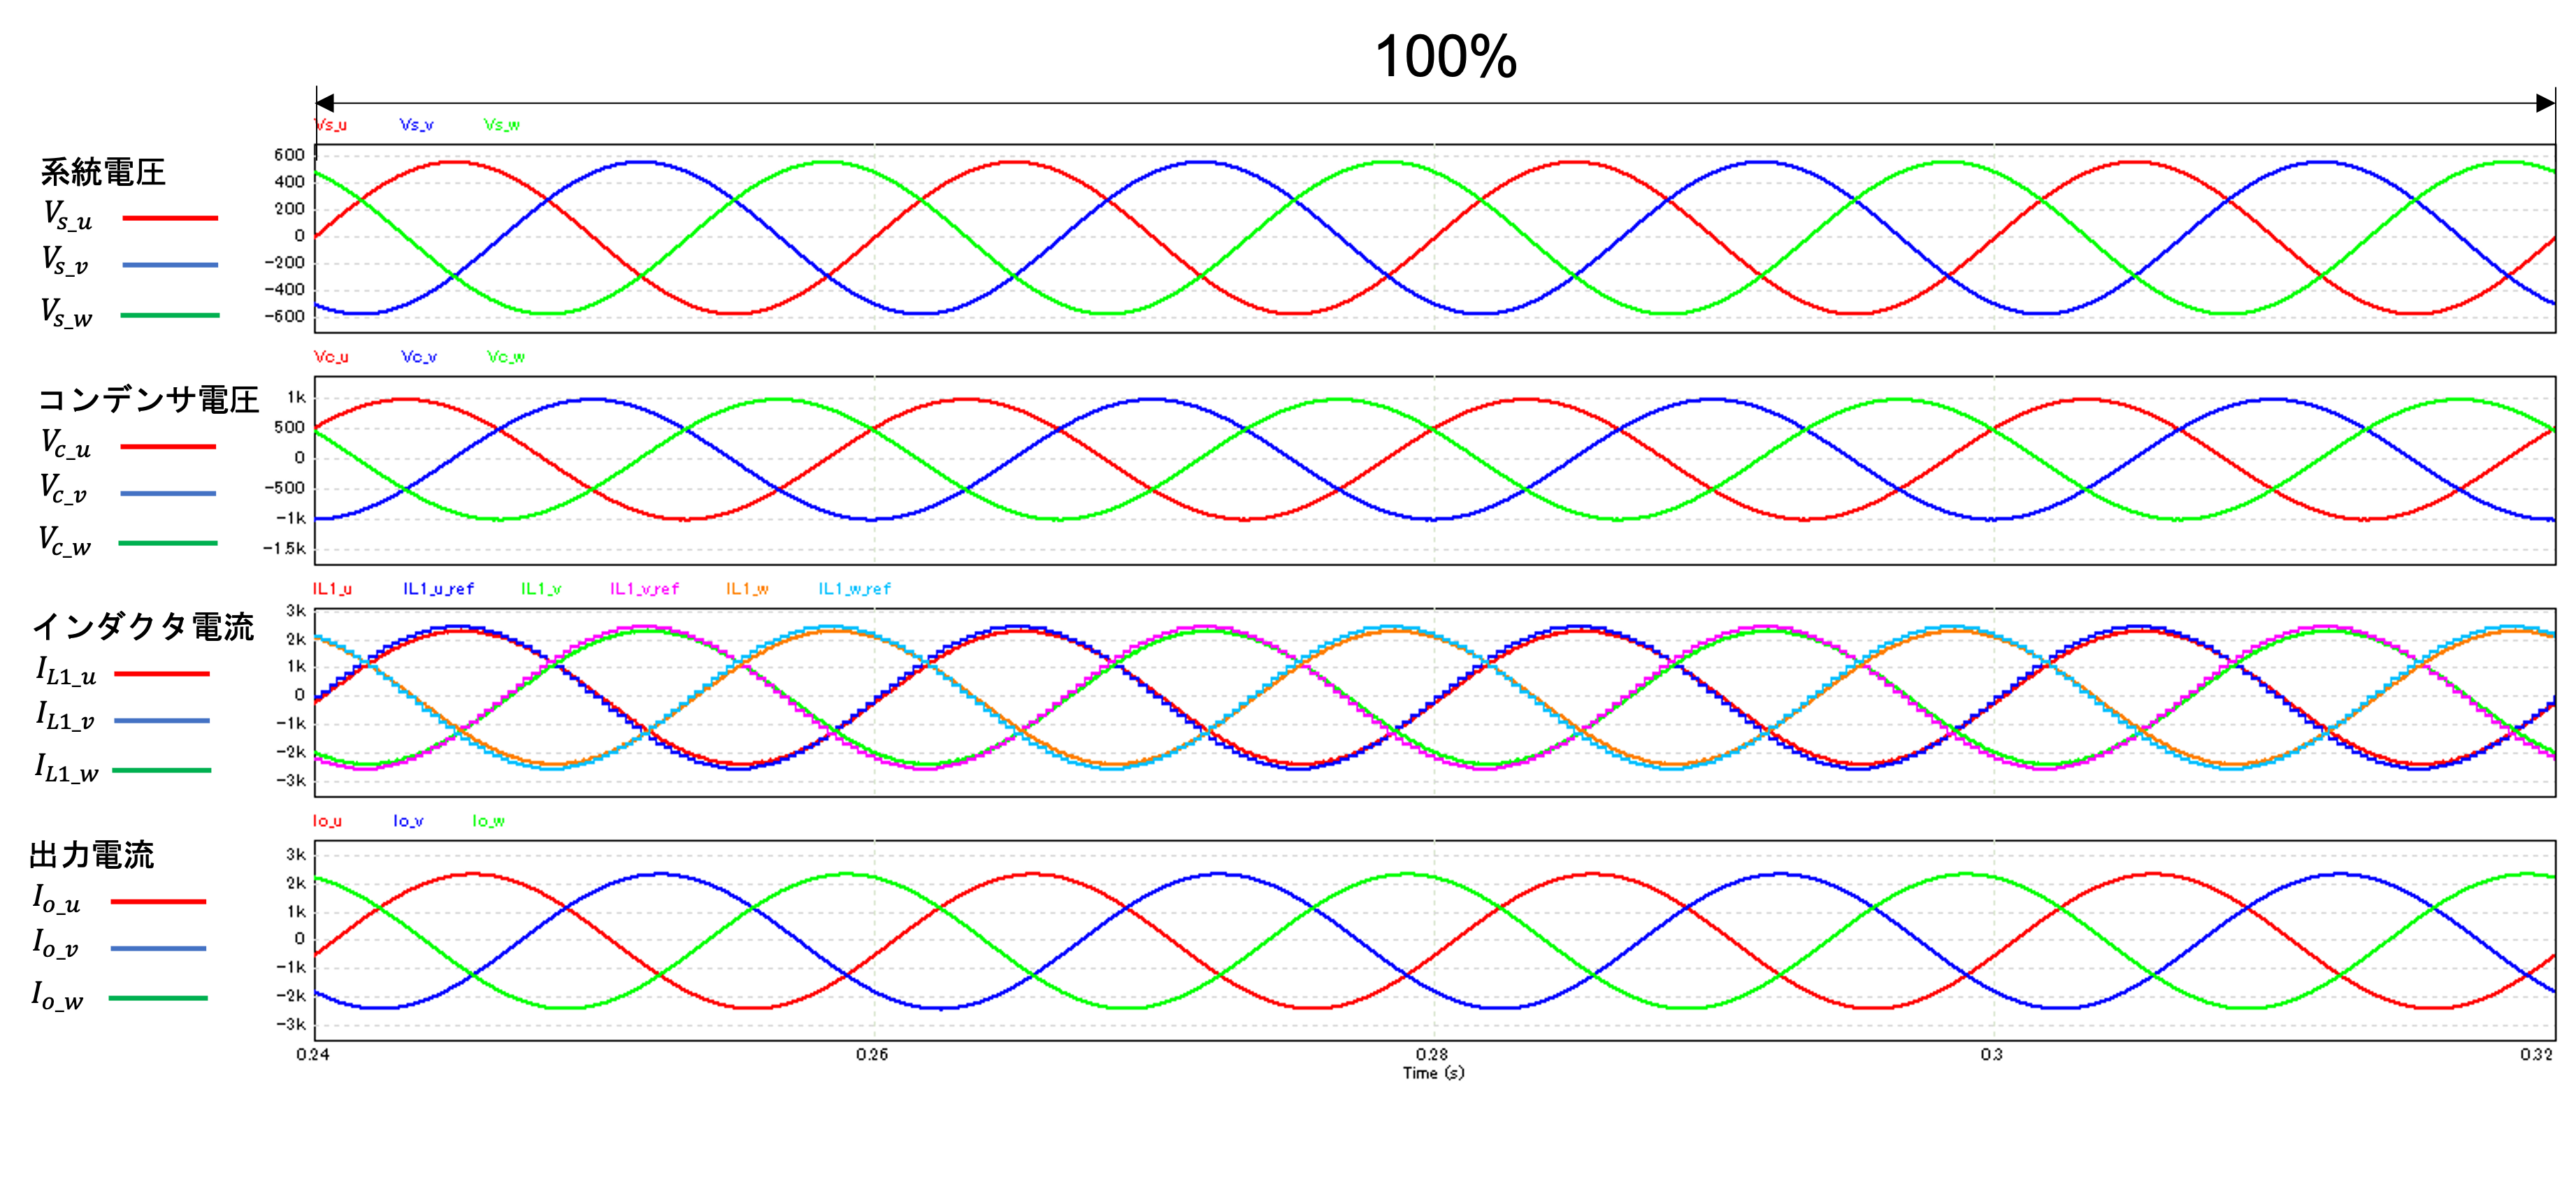
\includegraphics[width=140mm]{image/chapter3/Fig3.1.png}
    \caption{定常運転時の出力波形}
    \label{Fig3.1}
\end{figure}

\newpage
\begin{figure}[ht]
    \center
    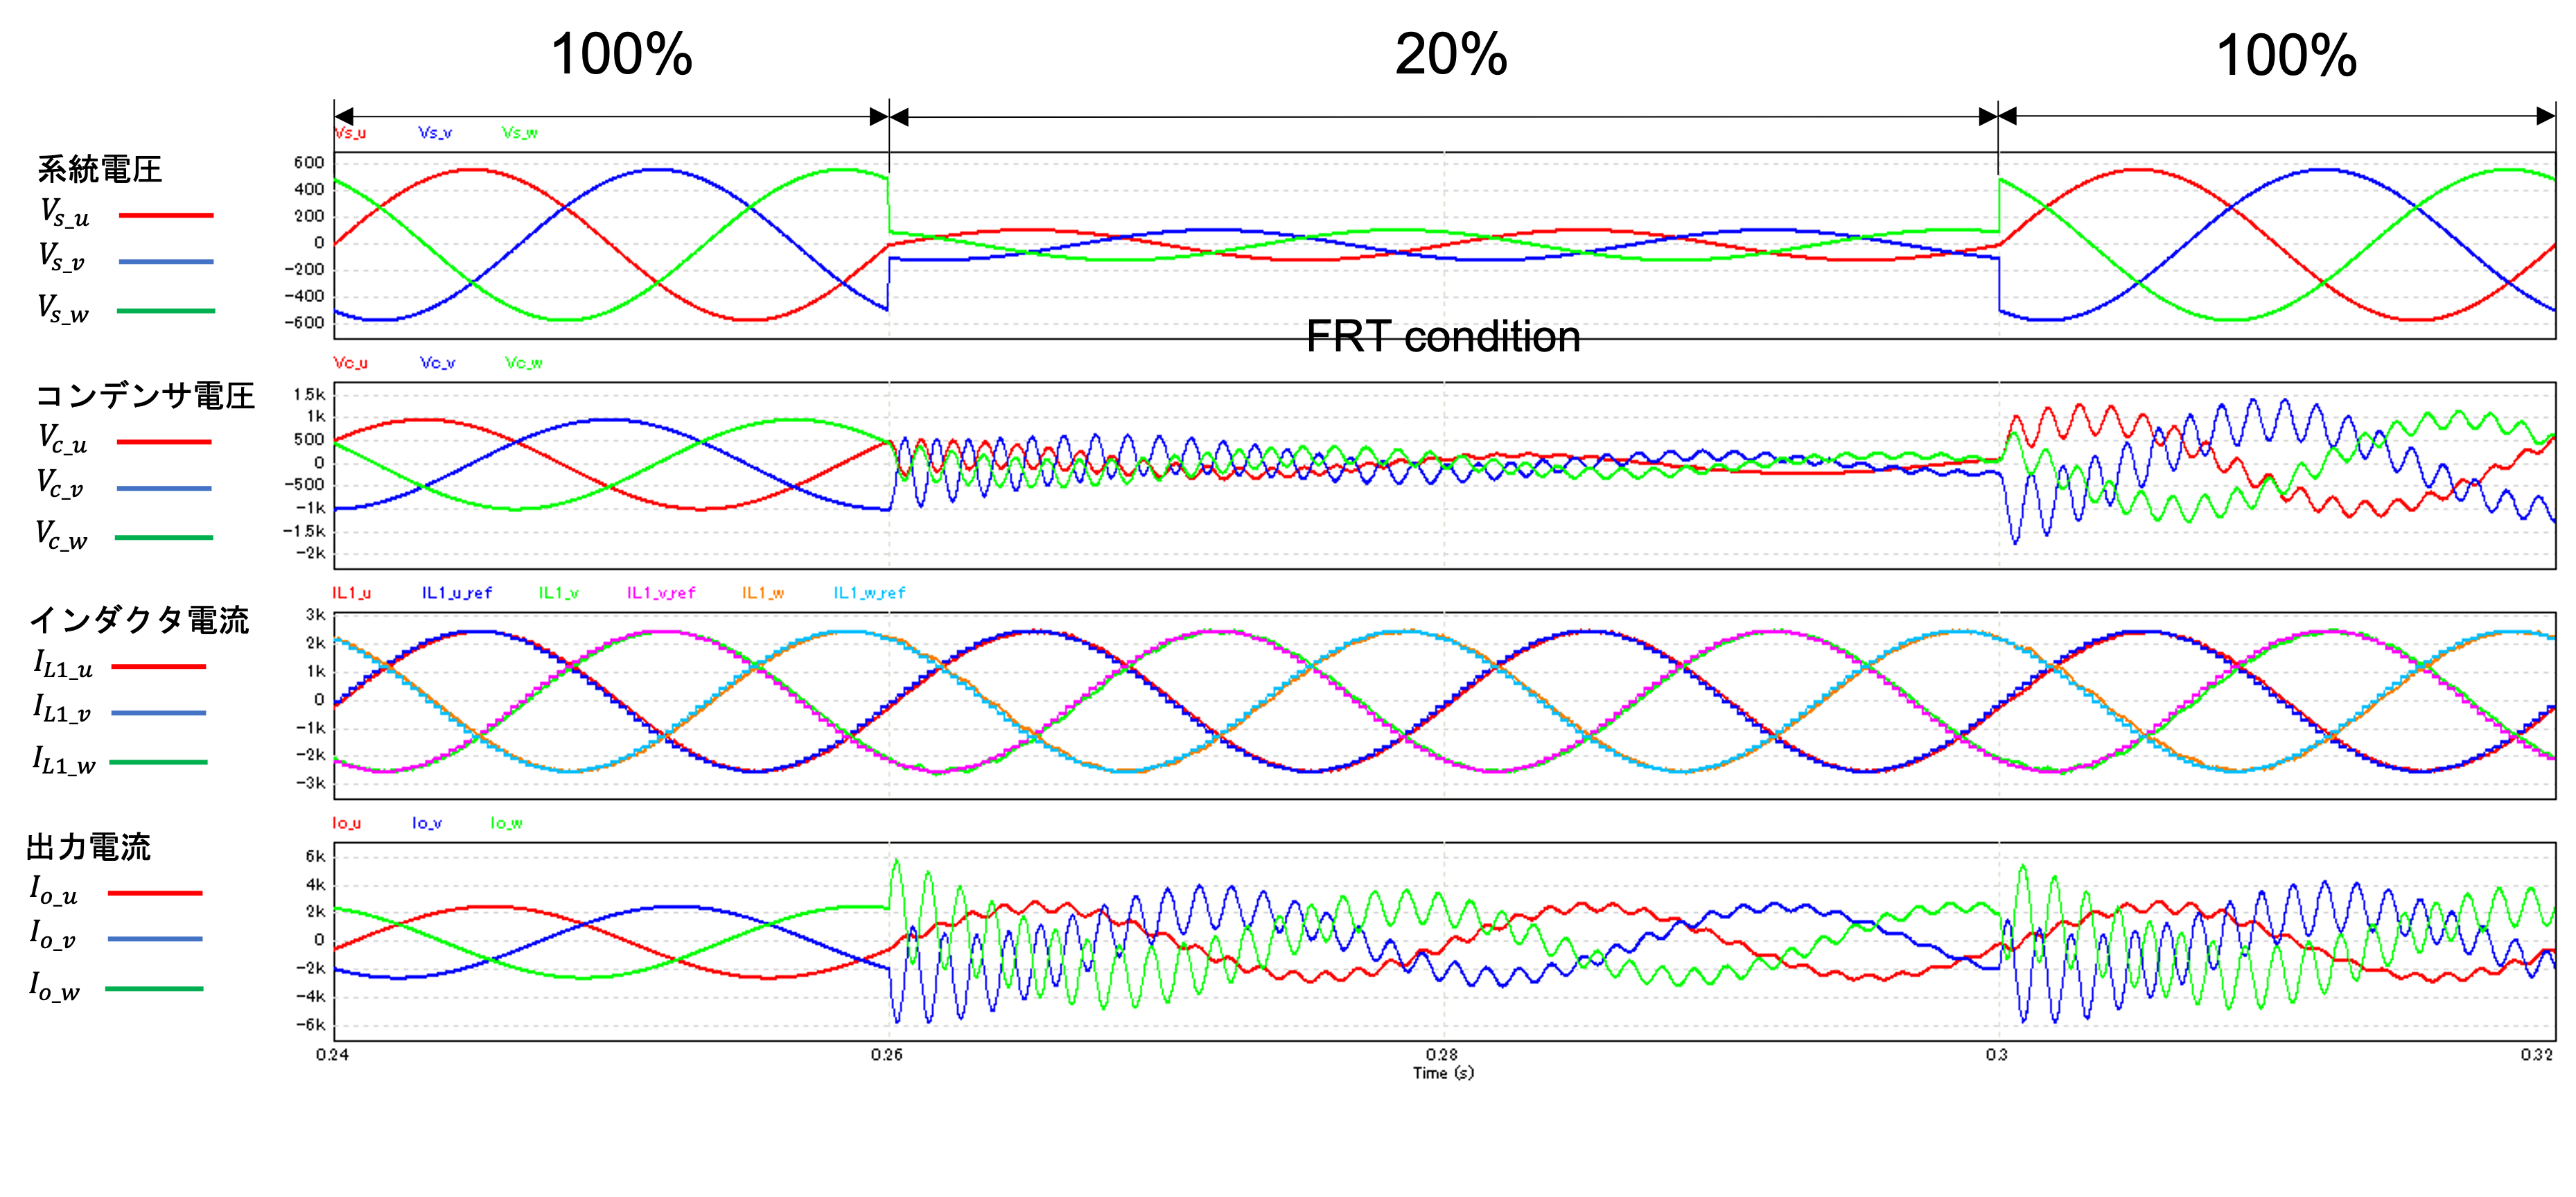
\includegraphics[width=140mm]{image/chapter3/Fig3.2.png}
    \caption{系統擾乱発生時の出力波形}
    \label{Fig3.2}
\end{figure}


表\ref{Tab3.3}にシミュレーション結果を示す．
\begin{table}[htb]
\centering
  \caption{シミュレーション結果}
  \begin{tabular}{c|c|c|c}  \hline\hline 
    \multirow{2}{*}{Condition}& \multicolumn{3}{|c}{THD [\%]} \\  \cline{2-4}
     & U相 & V相  & W相\\  \hline 
    定常時 & 0.88 & 0.90 & 0.93 \\ 
    系統擾乱発生時 & 0.77 & 1.02 & 1.17 \\ \hline
  \end{tabular}
  \label{Tab3.3}
\end{table}

表\ref{Tab3.3}より，定常運転時に対して系統擾乱発生時でTHDがそれぞれ，U相で13\%減少，V相で13\%増加，W相で25\%で増加していることがわかる．\\
外乱補償型マルチサンプリングデッドビート制御の定常運転時と系統擾乱発生時の出力応答を示す．

\begin{figure}[ht]
    \center
    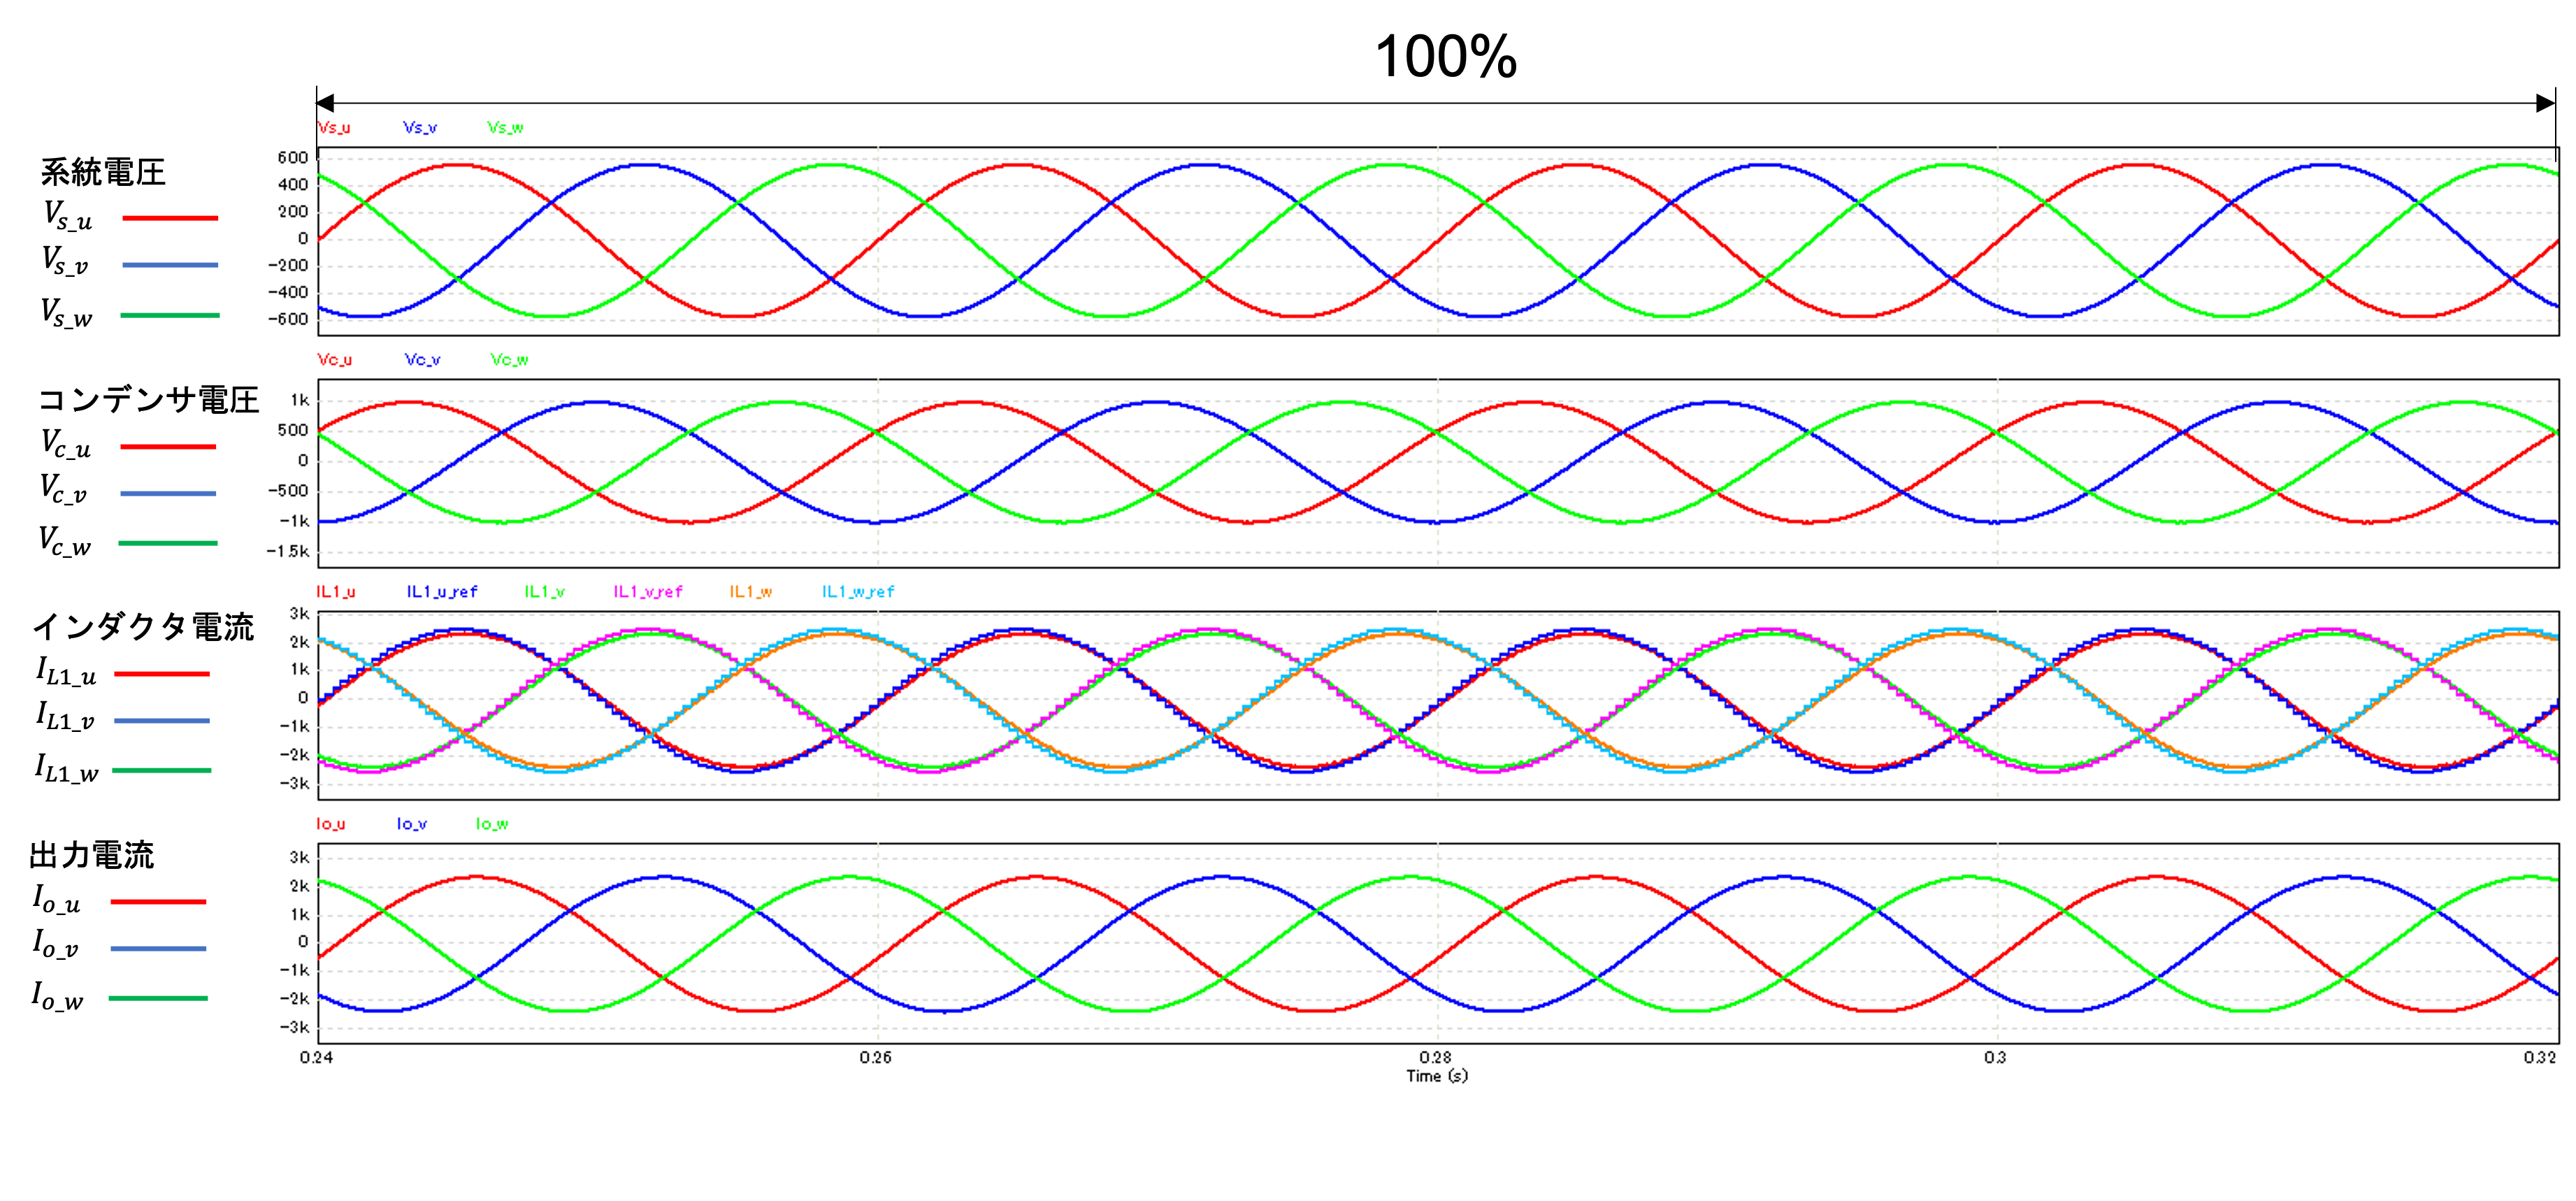
\includegraphics[width=140mm]{image/chapter3/Fig3.3.png}
    \caption{定常運転時の出力波形}
    \label{Fig3.3}
\end{figure}

\begin{figure}[ht]
    \center
    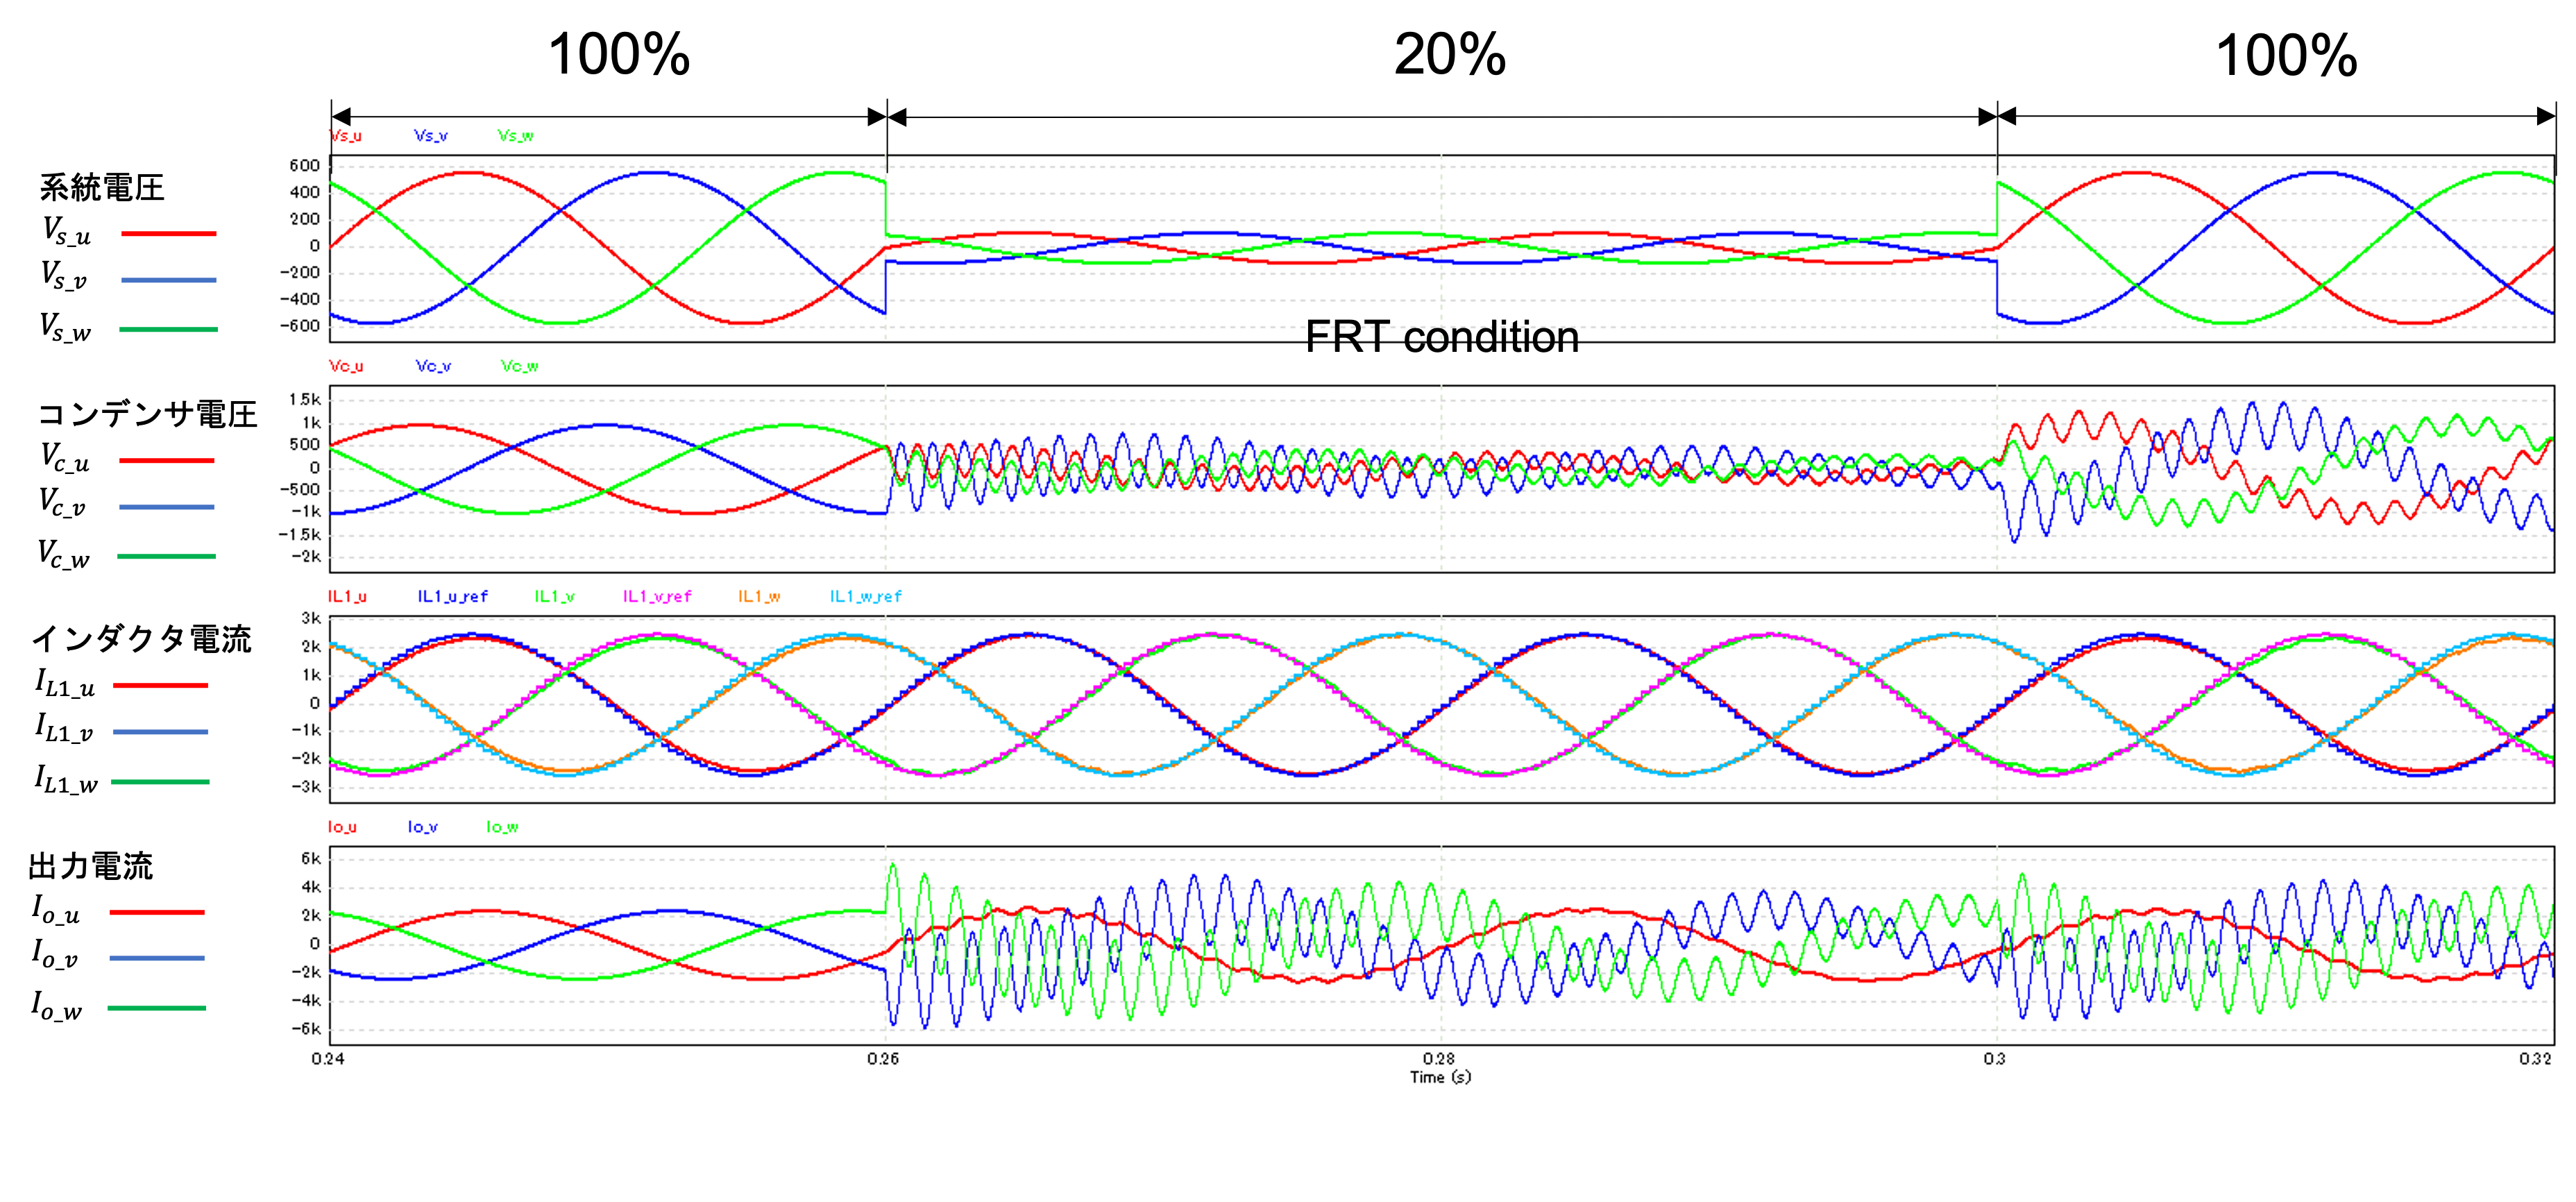
\includegraphics[width=140mm]{image/chapter3/Fig3.4.png}
    \caption{系統擾乱発生時の出力波形}
    \label{Fig3.4}
\end{figure}

\newpage

表\ref{Tab3.4}にシミュレーション結果を示す．
\begin{table}[htb]
\centering
  \caption{シミュレーション結果}
  \begin{tabular}{c|c|c|c}  \hline\hline 
    \multirow{2}{*}{Condition}& \multicolumn{3}{|c}{THD [\%]} \\  \cline{2-4}
     & U相 & V相  & W相\\  \hline 
    定常時 & 0.89 & 0.88 & 0.88 \\ 
    系統擾乱発生時 & 0.75 & 1.46 & 1.46 \\ \hline
  \end{tabular}
  \label{Tab3.4}
\end{table}

表\ref{Tab3.4}より，定常運転時に対して系統擾乱発生時でTHDがそれぞれ，U相で19\%減少，V相で22\%増加，W相で22\%で増加していることがわかる．\\

\subsection{アンノミナル検証}
パターン1のときの外乱補償型シングルレートデッドビート制御の出力応答波形を示す．
\newpage

\begin{figure}[ht]
    \center
    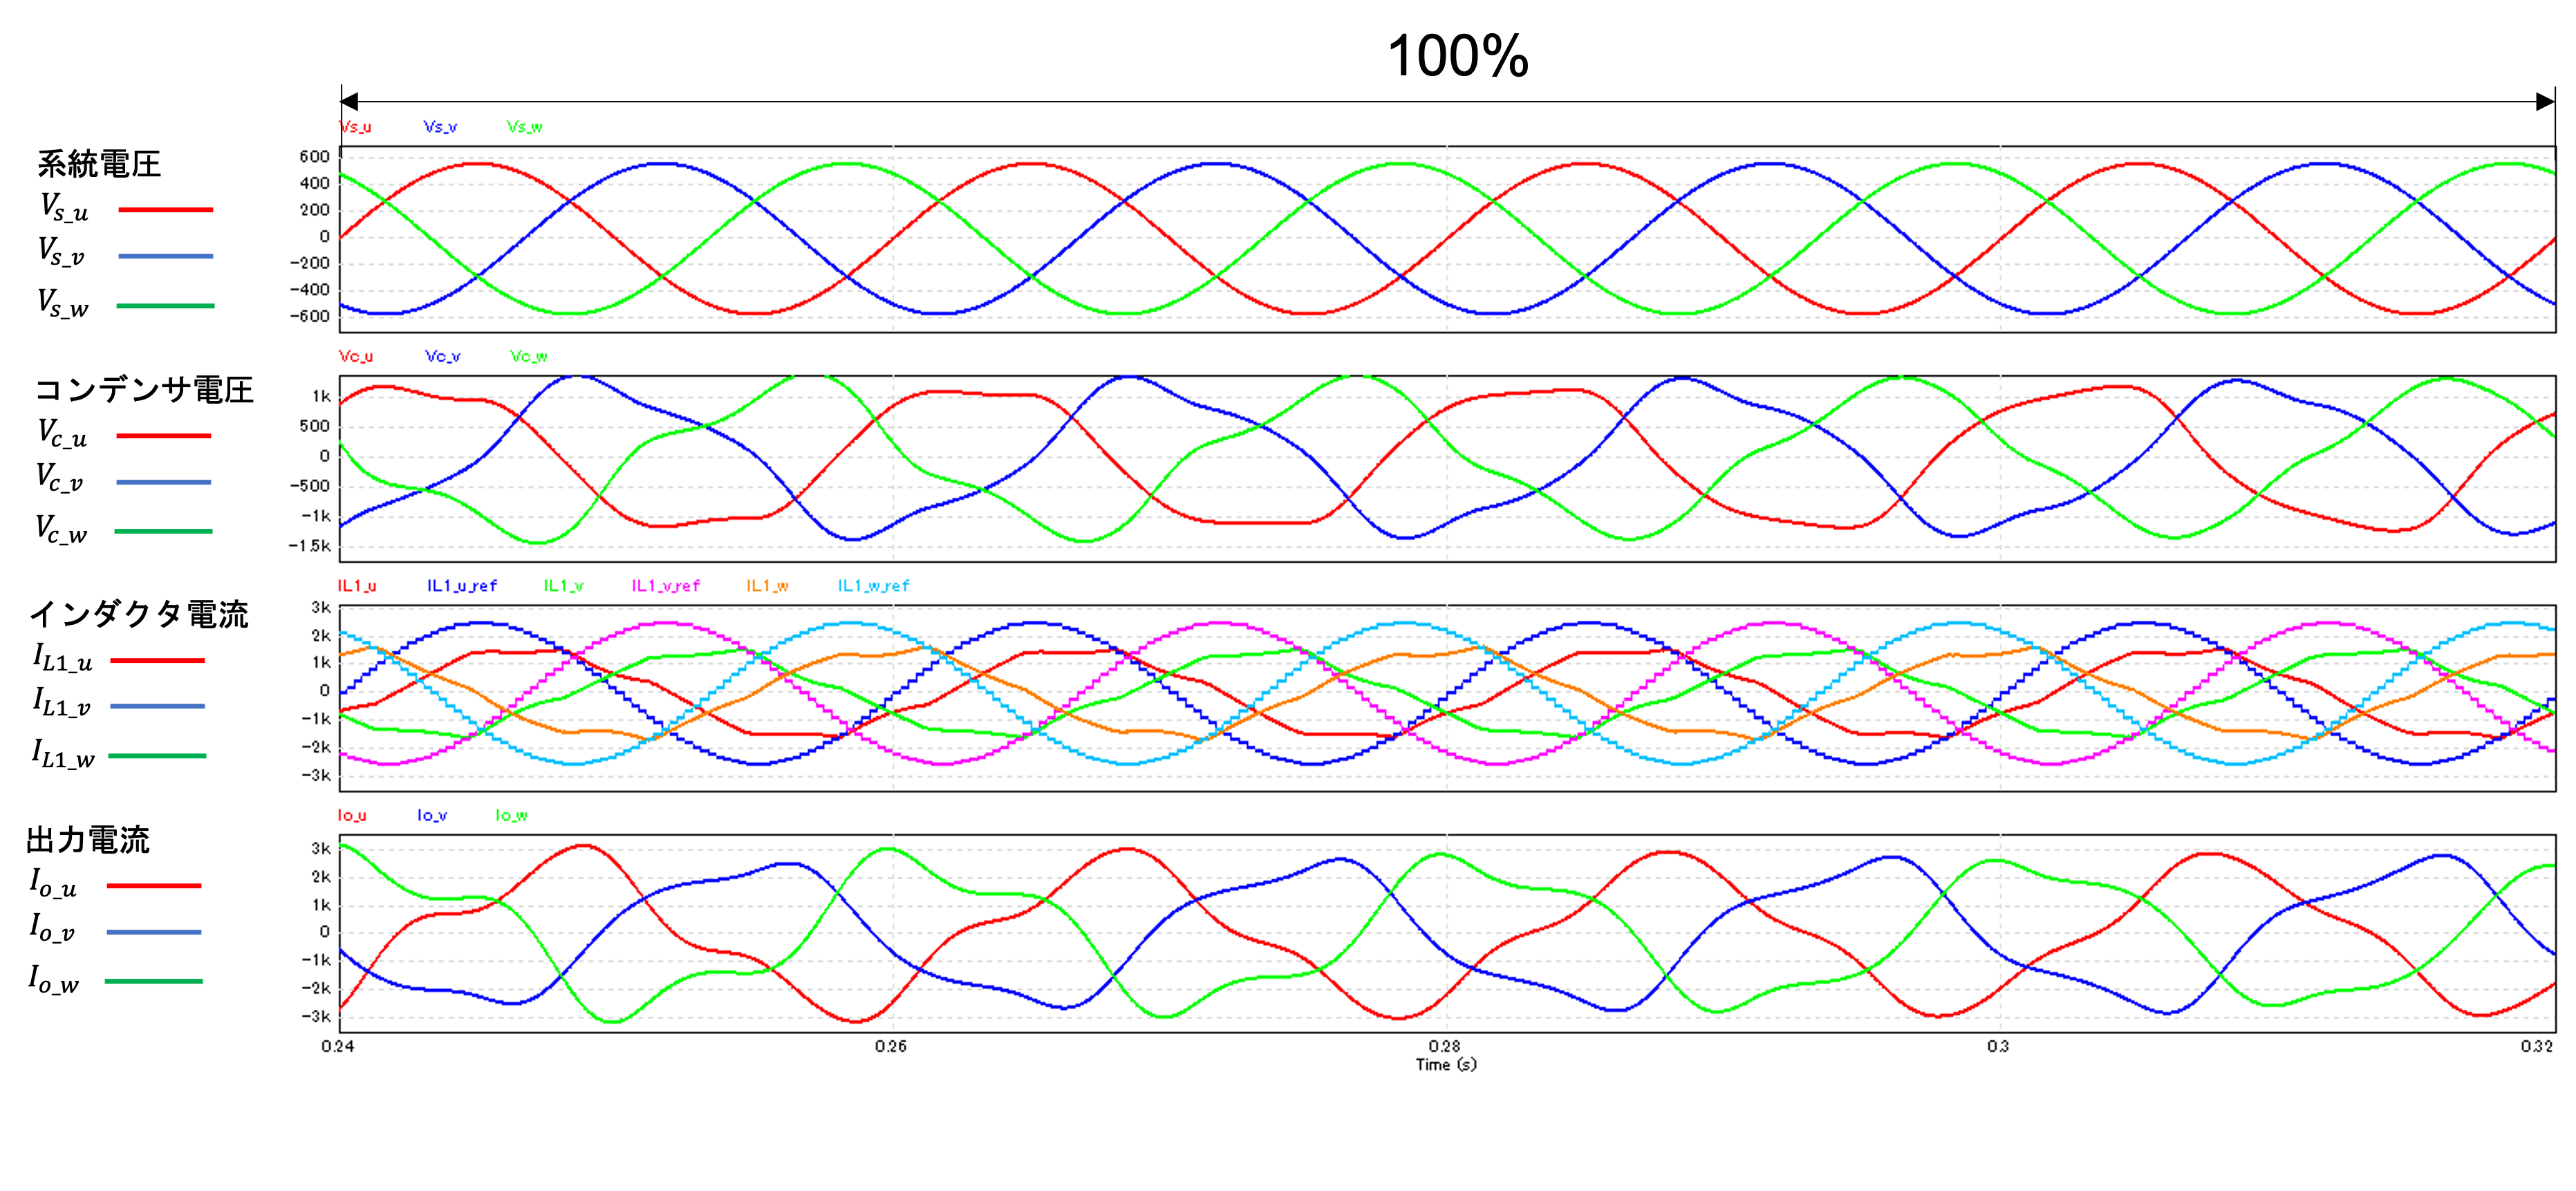
\includegraphics[width=140mm]{image/chapter3/Fig3.5.png}
    \caption{定常運転時(パターン1)}
    \label{Fig3.5}
\end{figure}

\begin{figure}[ht]
    \center
    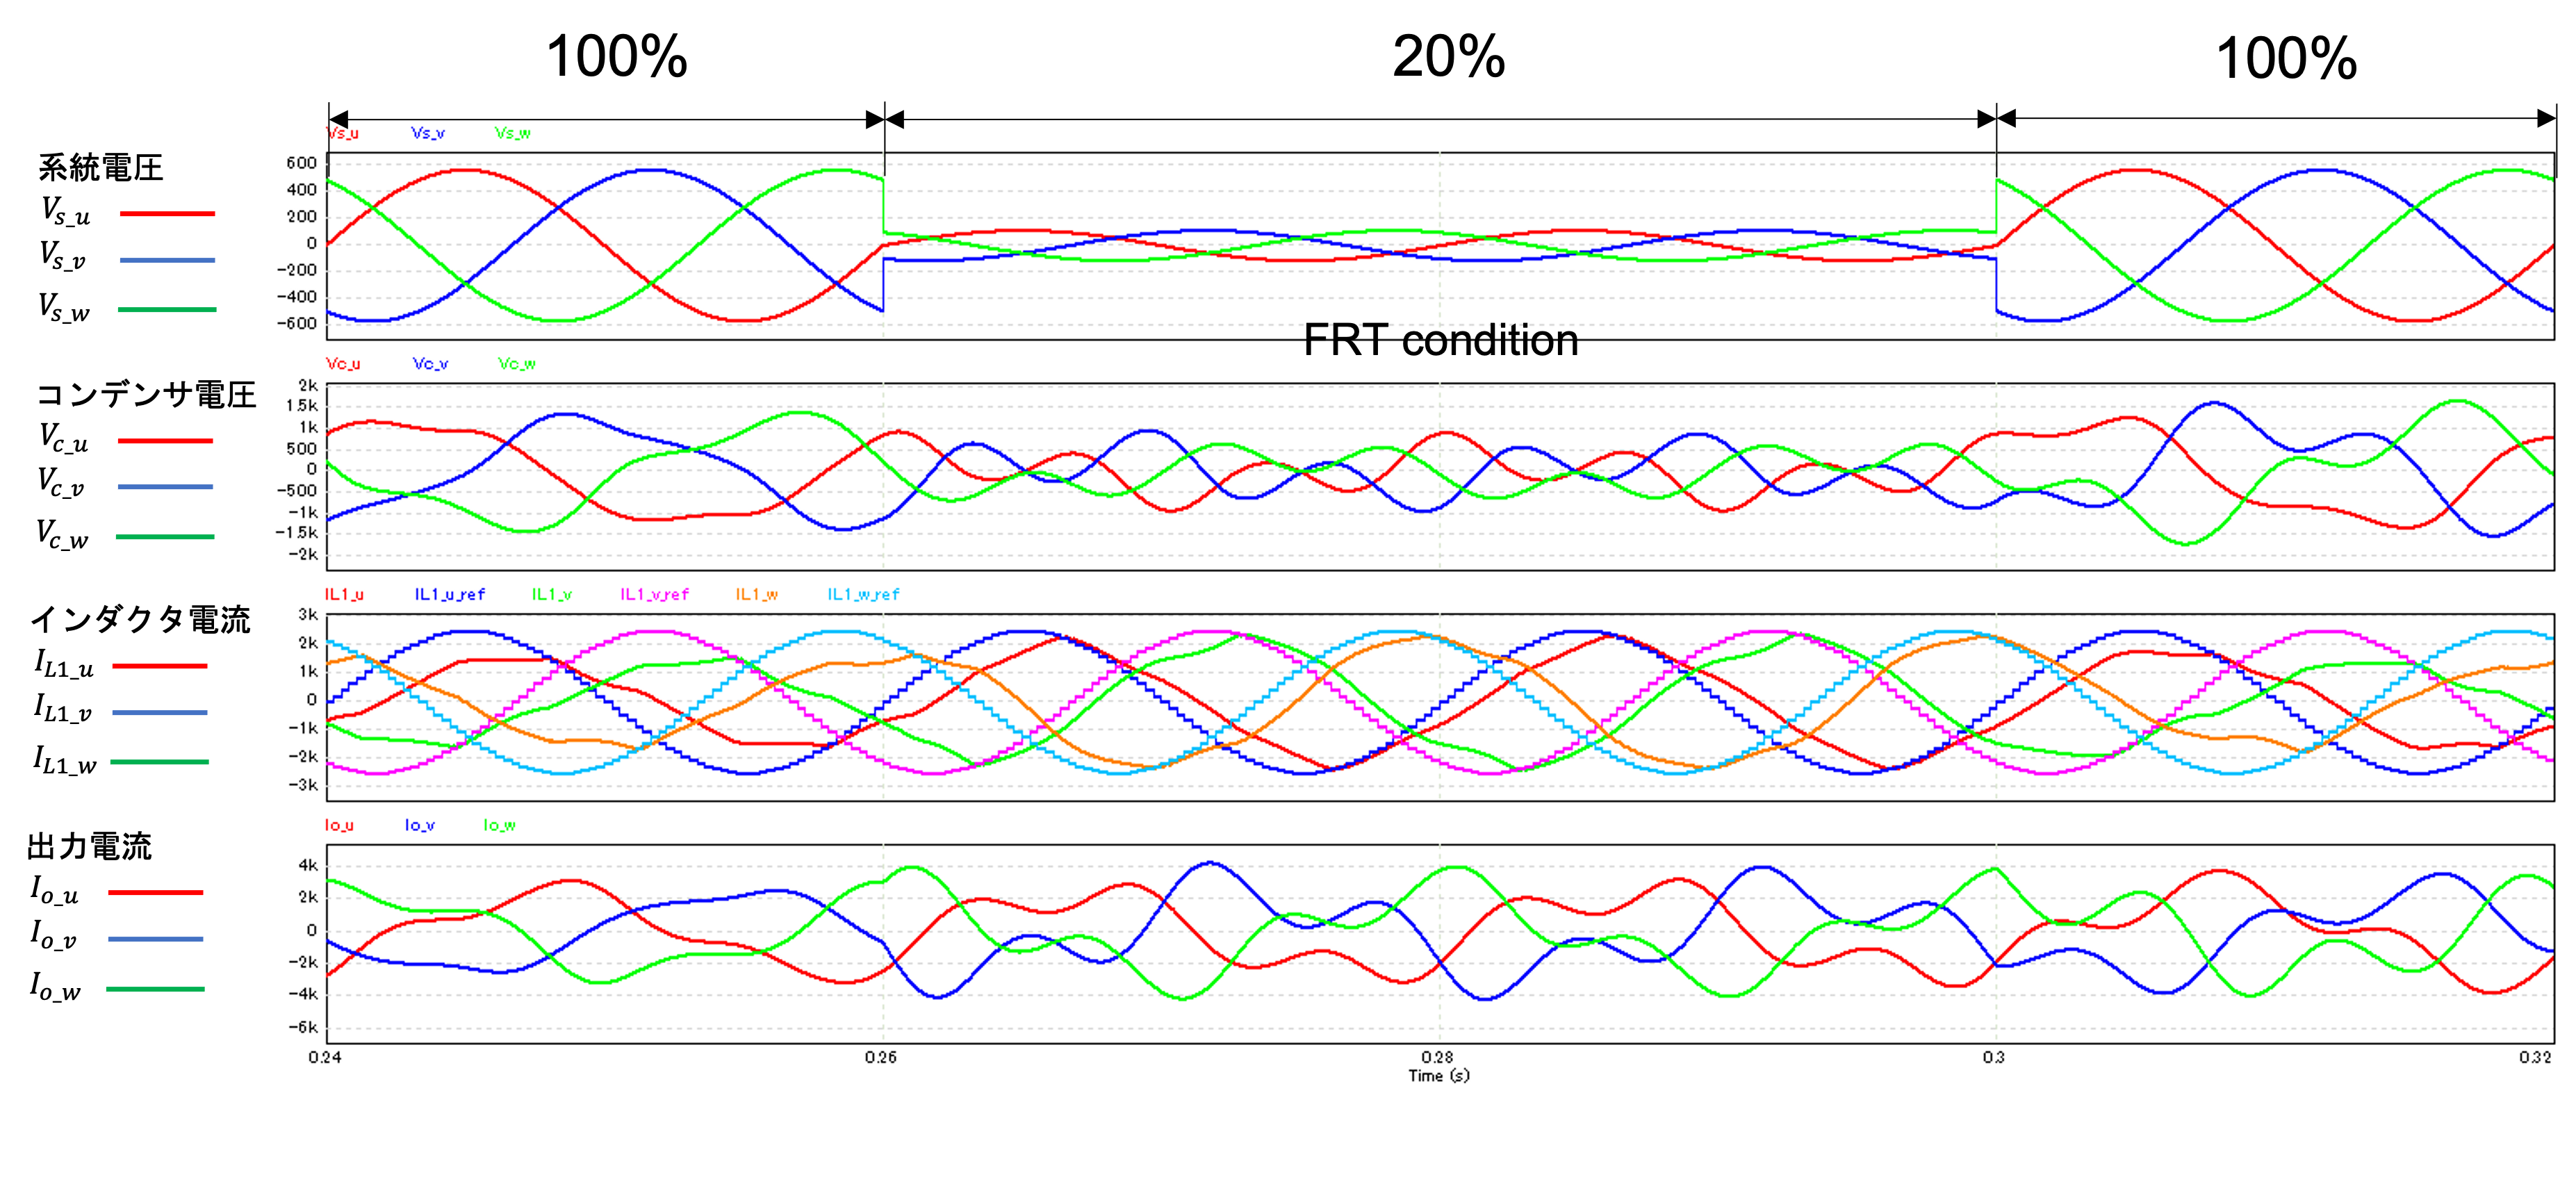
\includegraphics[width=140mm]{image/chapter3/Fig3.6.png}
    \caption{系統擾乱発生時(パターン1)}
    \label{Fig3.6}
\end{figure}

表\ref{Tab3.5}にシミュレーション結果を示す．
\begin{table}[htb]
\centering
  \caption{シミュレーション結果}
  \begin{tabular}{c|c|c|c}  \hline\hline 
    \multirow{2}{*}{Condition}& \multicolumn{3}{|c}{THD [\%]} \\  \cline{2-4}
     & U相 & V相  & W相\\  \hline 
    定常時 & 8.37 & 9.11 & 8.95 \\ 
    系統擾乱発生時 & 7.35 & 8.36 & 7.31 \\ \hline
  \end{tabular}
  \label{Tab3.5}
\end{table}

表\ref{Tab3.5}から，定常運転時と系統擾乱発生時の場合において制御量であるインダクタ電流$I_{L1}$を制御することが出来ていないことがわかる．また，THDはFRT要件で定められている5\%を満たしていないことがわかる．定常運転時に対して系統擾乱発生時でTHDがそれぞれU相で12\%減少，V相で8\%減少，W相で18\%減少していることがわかる．\\
パターン2のときの外乱補償型シングルレートデッドビート制御の出力応答波形を示す．

\begin{figure}[ht]
    \center
    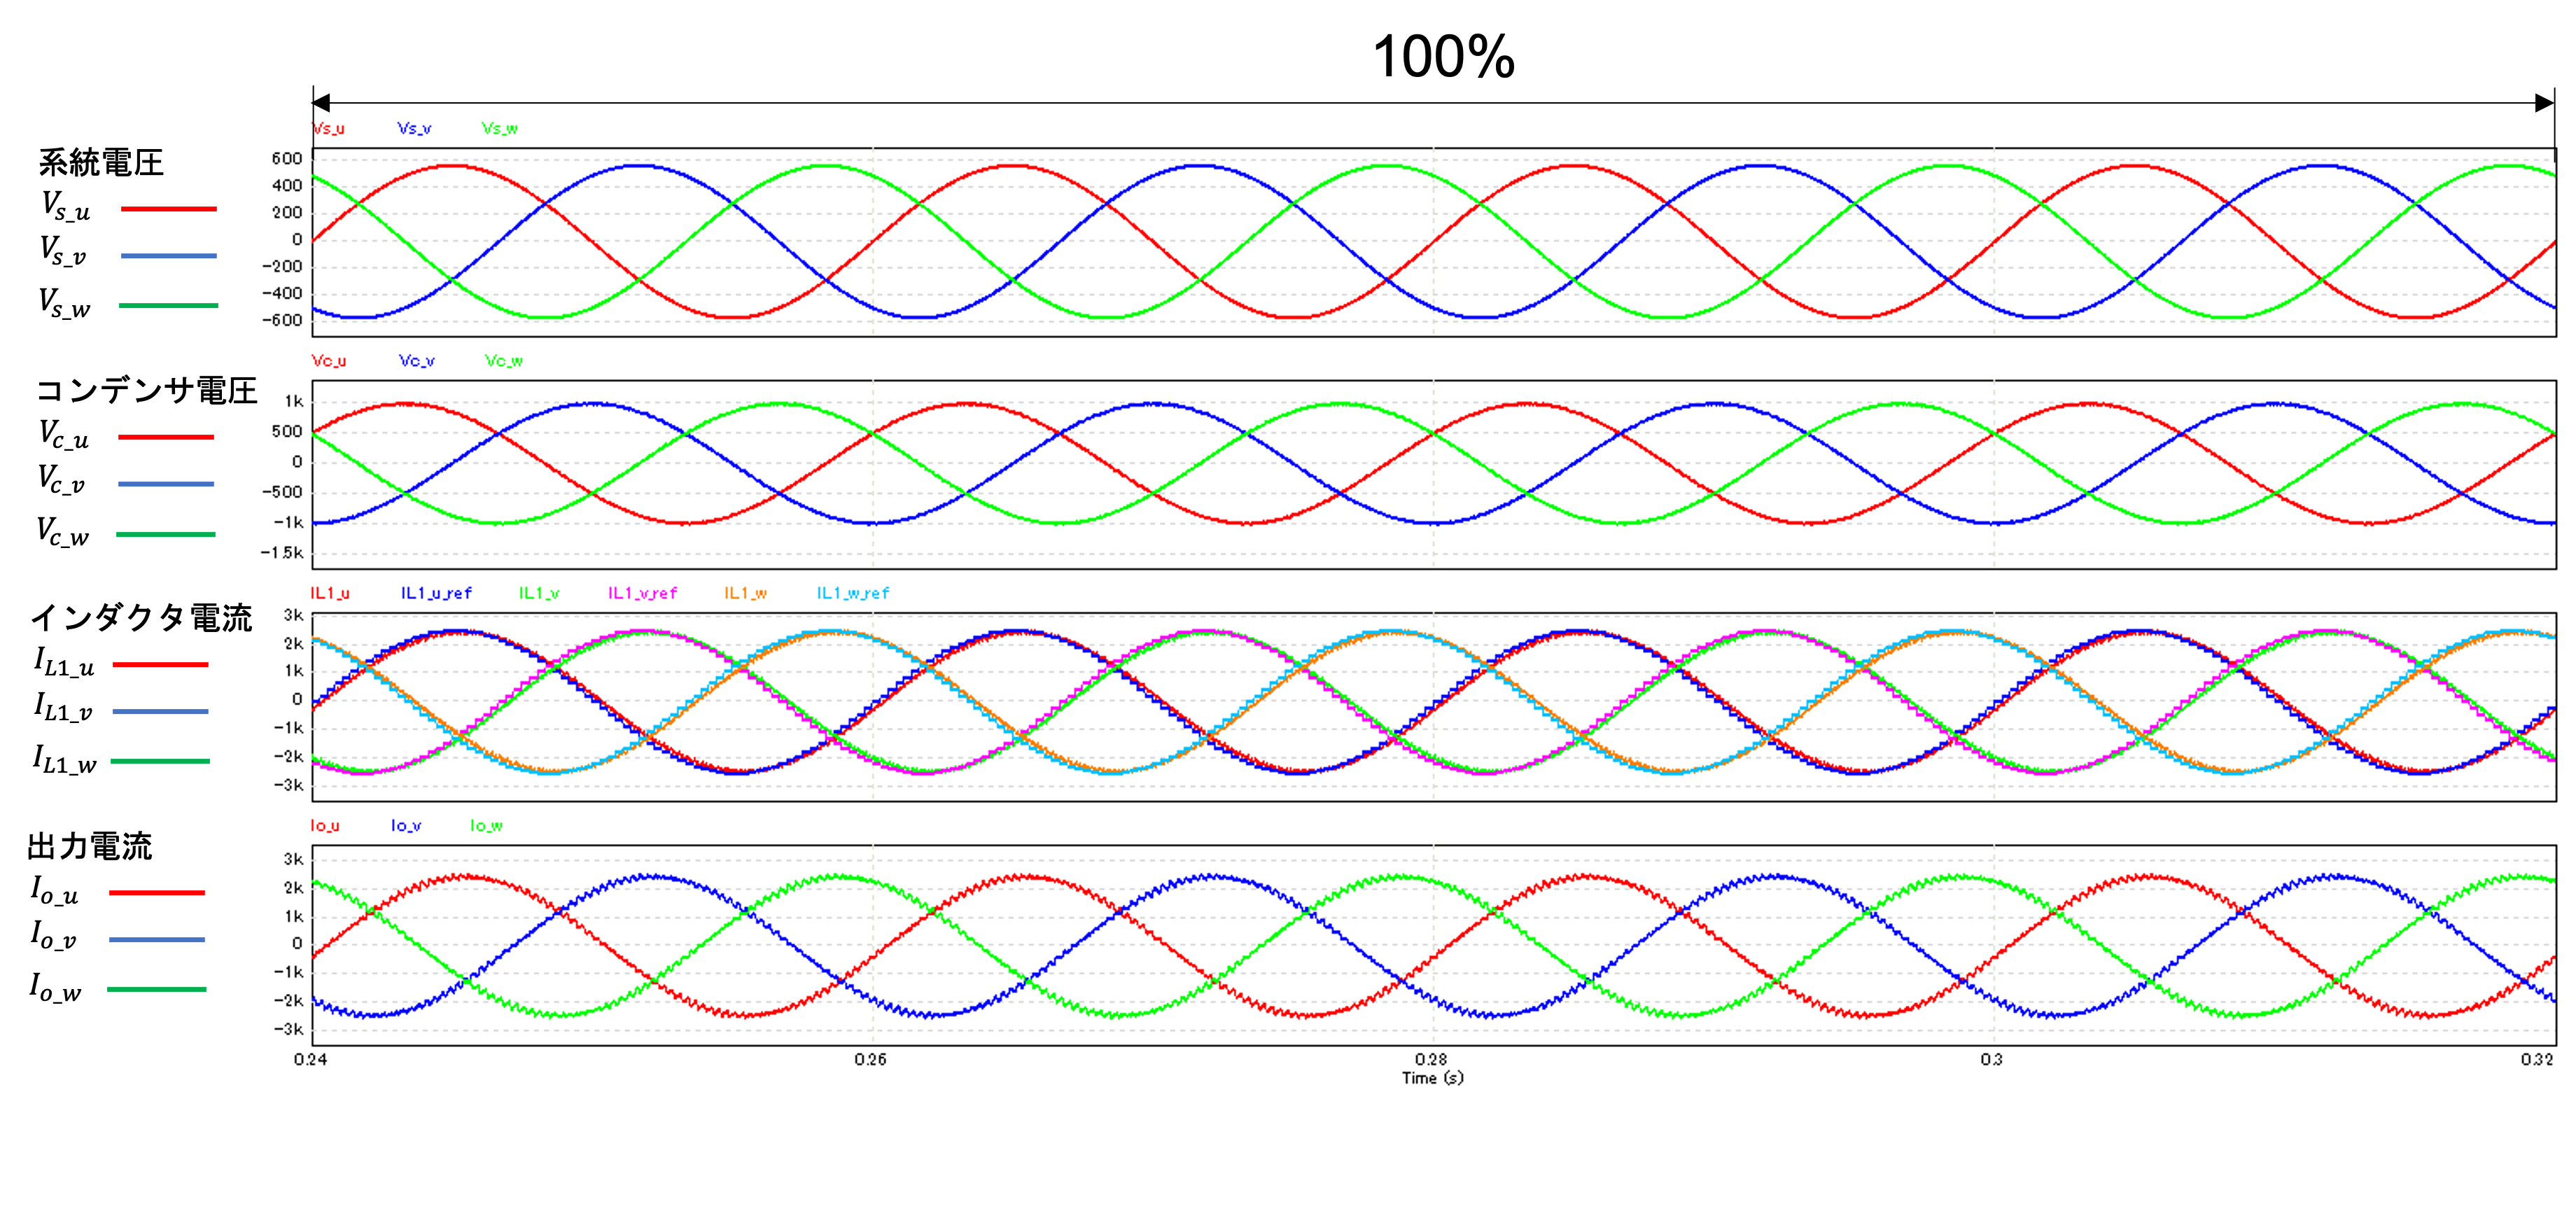
\includegraphics[width=140mm]{image/chapter3/Fig3.7.png}
    \caption{定常運転時(パターン2)}
    \label{Fig3.7}
\end{figure}

\begin{figure}[ht]
    \center
    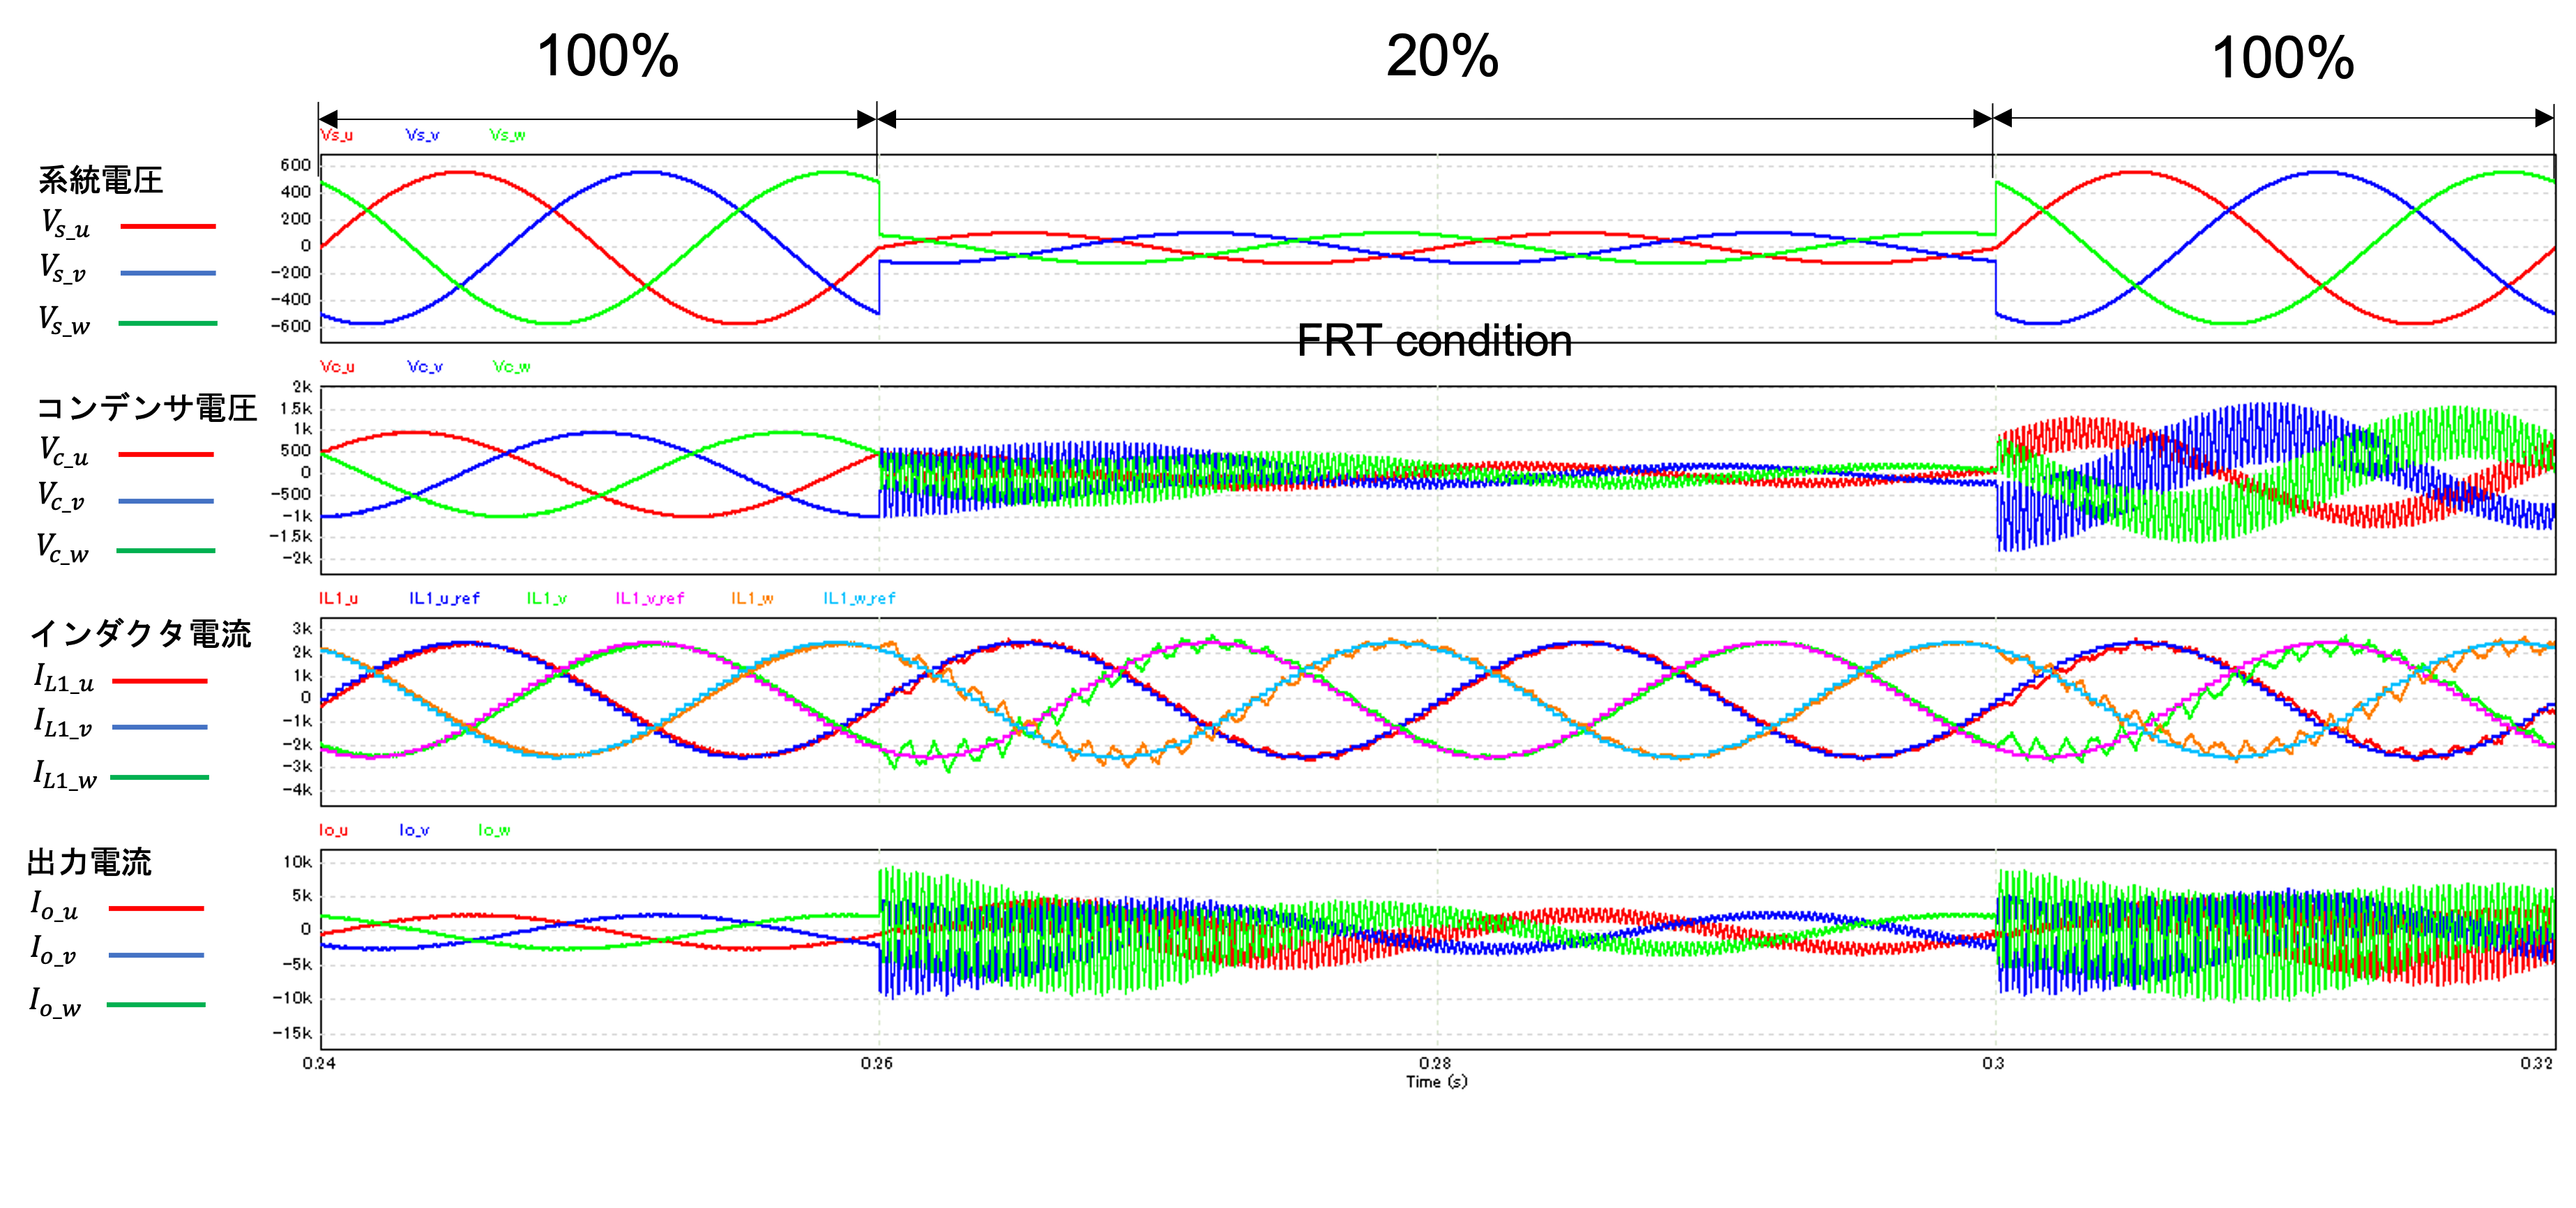
\includegraphics[width=140mm]{image/chapter3/Fig3.8.png}
    \caption{系統擾乱発生時(パターン2)}
    \label{Fig3.8}
\end{figure}

\newpage

表\ref{Tab3.6}にシミュレーション結果を示す．
\begin{table}[htb]
\centering
  \caption{シミュレーション結果}
  \begin{tabular}{c|c|c|c}  \hline\hline 
    \multirow{2}{*}{Condition}& \multicolumn{3}{|c}{THD [\%]} \\  \cline{2-4}
     & U相 & V相  & W相\\  \hline 
    定常時 & 18.4 & 18.5 & 18.6 \\ 
    系統擾乱発生時 & 28.9 & 22.4 & 41.9 \\ \hline
  \end{tabular}
  \label{Tab3.6}
\end{table}

表\ref{Tab3.6}から，定常運転時と系統擾乱発生時の場合において制御量であるインダクタ電流$I_{L1}$を制御することが出来ているわかる．一方で定常運転時，系統擾乱発生時のTHDはFRT要件で定められている5\%を満たしていないことがわかる．常運転時に対して系統擾乱発生時でTHDがそれぞれU相で57\%増加，V相で21\%増加，W相で125\%増加していることがわかる．\\
さらに，コンデンサ電圧$V_{c}$，出力電流$I_{o}$でフィルタ共振を起こしていることが確認できた．

パターン1のときの外乱補償型マルチサンプリングデッドビート制御の出力応答波形を示す．

\begin{figure}[ht]
    \center
    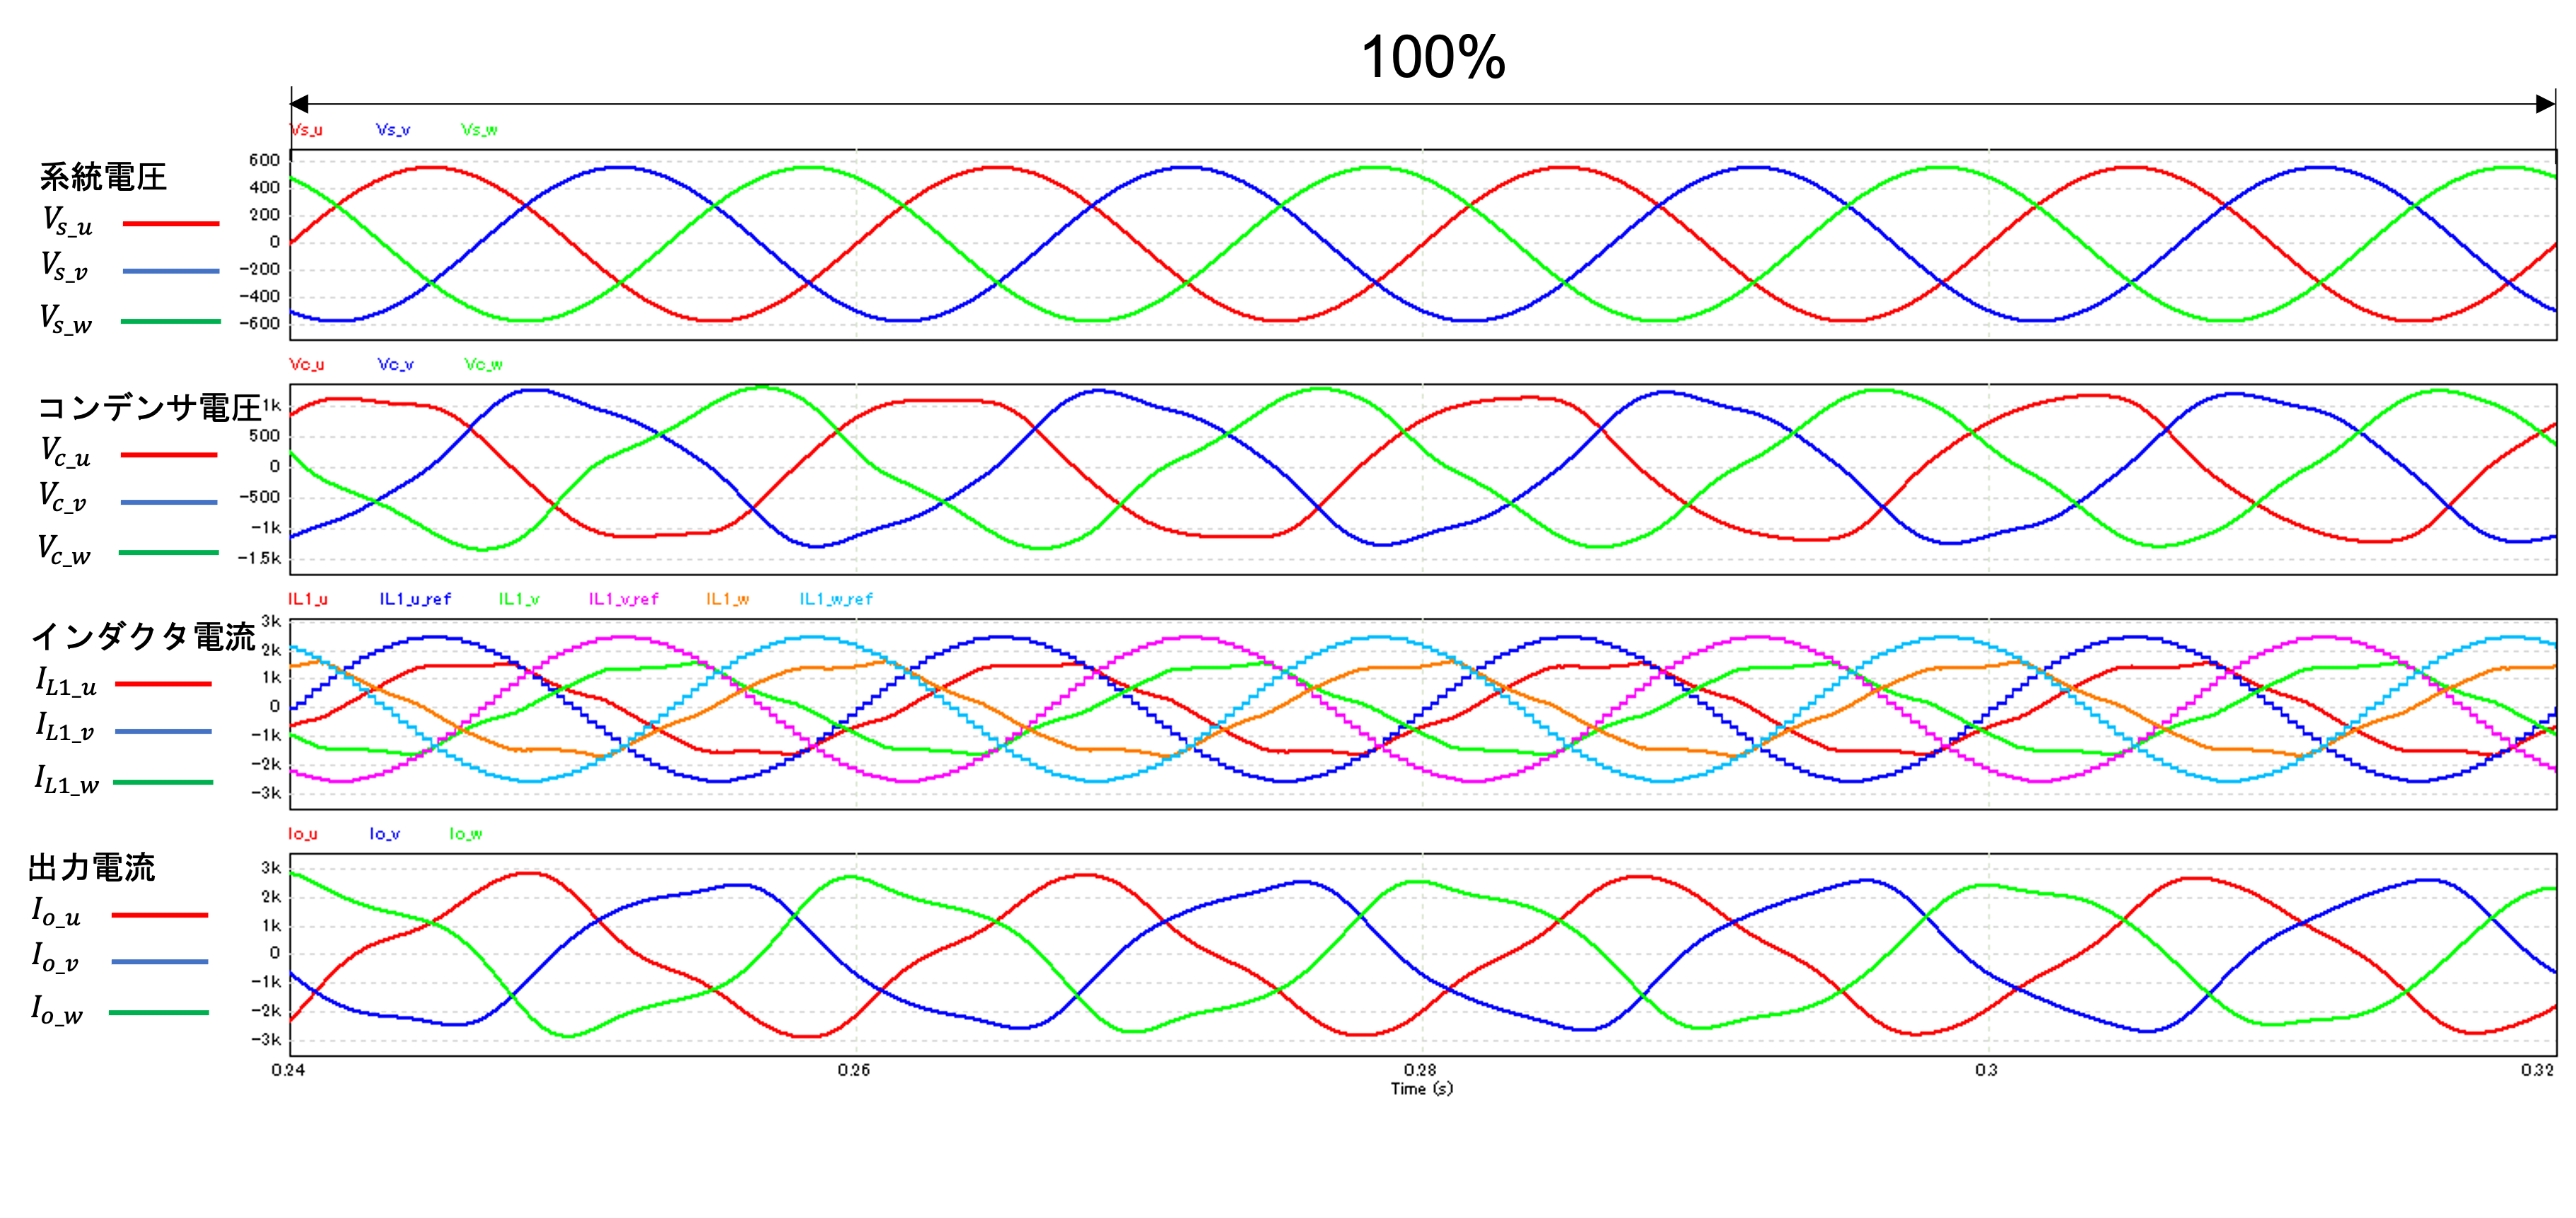
\includegraphics[width=140mm]{image/chapter3/Fig3.9.png}
    \caption{定常運転時(パターン1)}
    \label{Fig3.9}
\end{figure}

\begin{figure}[ht]
    \center
    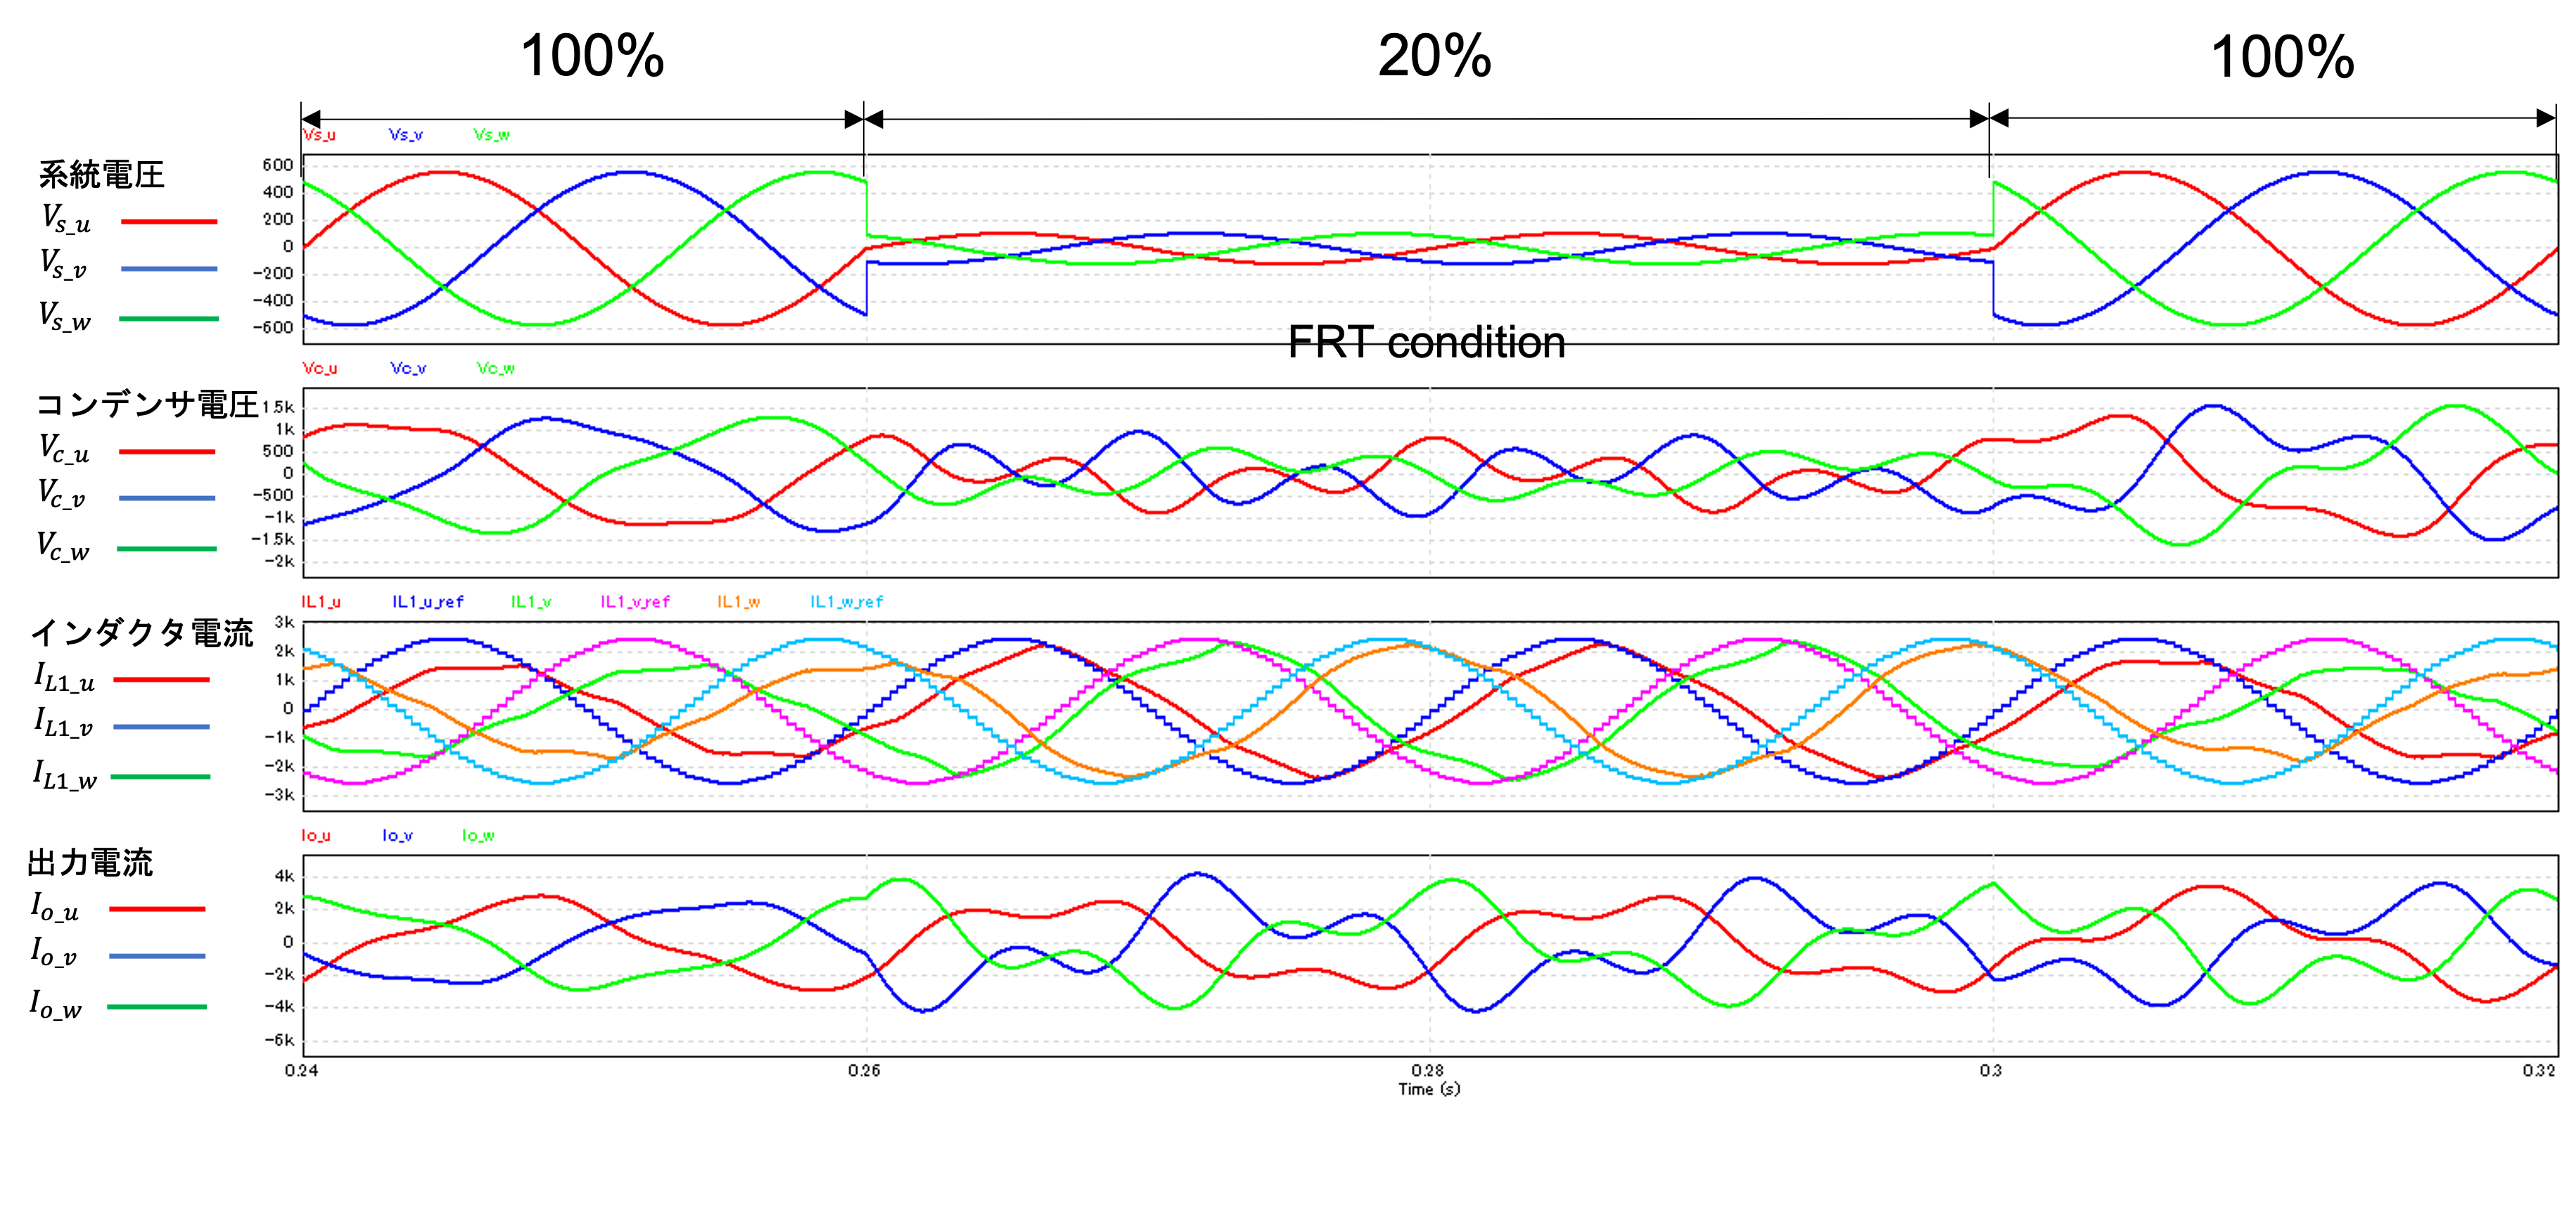
\includegraphics[width=140mm]{image/chapter3/Fig3.10.png}
    \caption{系統擾乱発生時(パターン1)}
    \label{Fig3.10}
\end{figure}

\newpage
表\ref{Tab3.7}にシミュレーション結果を示す．
\begin{table}[htb]
\centering
  \caption{シミュレーション結果}
  \begin{tabular}{c|c|c|c}  \hline\hline 
    \multirow{2}{*}{Condition}& \multicolumn{3}{|c}{THD [\%]} \\  \cline{2-4}
     & U相 & V相  & W相\\  \hline 
    定常時 & 7.40 & 7.76 & 7.75 \\ 
    系統擾乱発生時 & 6.08 & 8.42 & 6.86 \\ \hline
  \end{tabular}
  \label{Tab3.7}
\end{table}

表\ref{Tab3.7}から，定常運転時と系統擾乱発生時の場合において制御量であるインダクタ電流$I_{L1}$を制御することが出来ていないことがわかる．また，THDはFRT要件で定められている5\%を満たしていないことがわかる．定常運転時に対して系統擾乱発生時でTHDがそれぞれU相で18\%減少，V相で9\%増加，W相で11\%減少していることがわかる．\\
パターン2のときの外乱補償型マルチサンプリングデッドビート制御の出力応答波形を示す．

\begin{figure}[ht]
    \center
    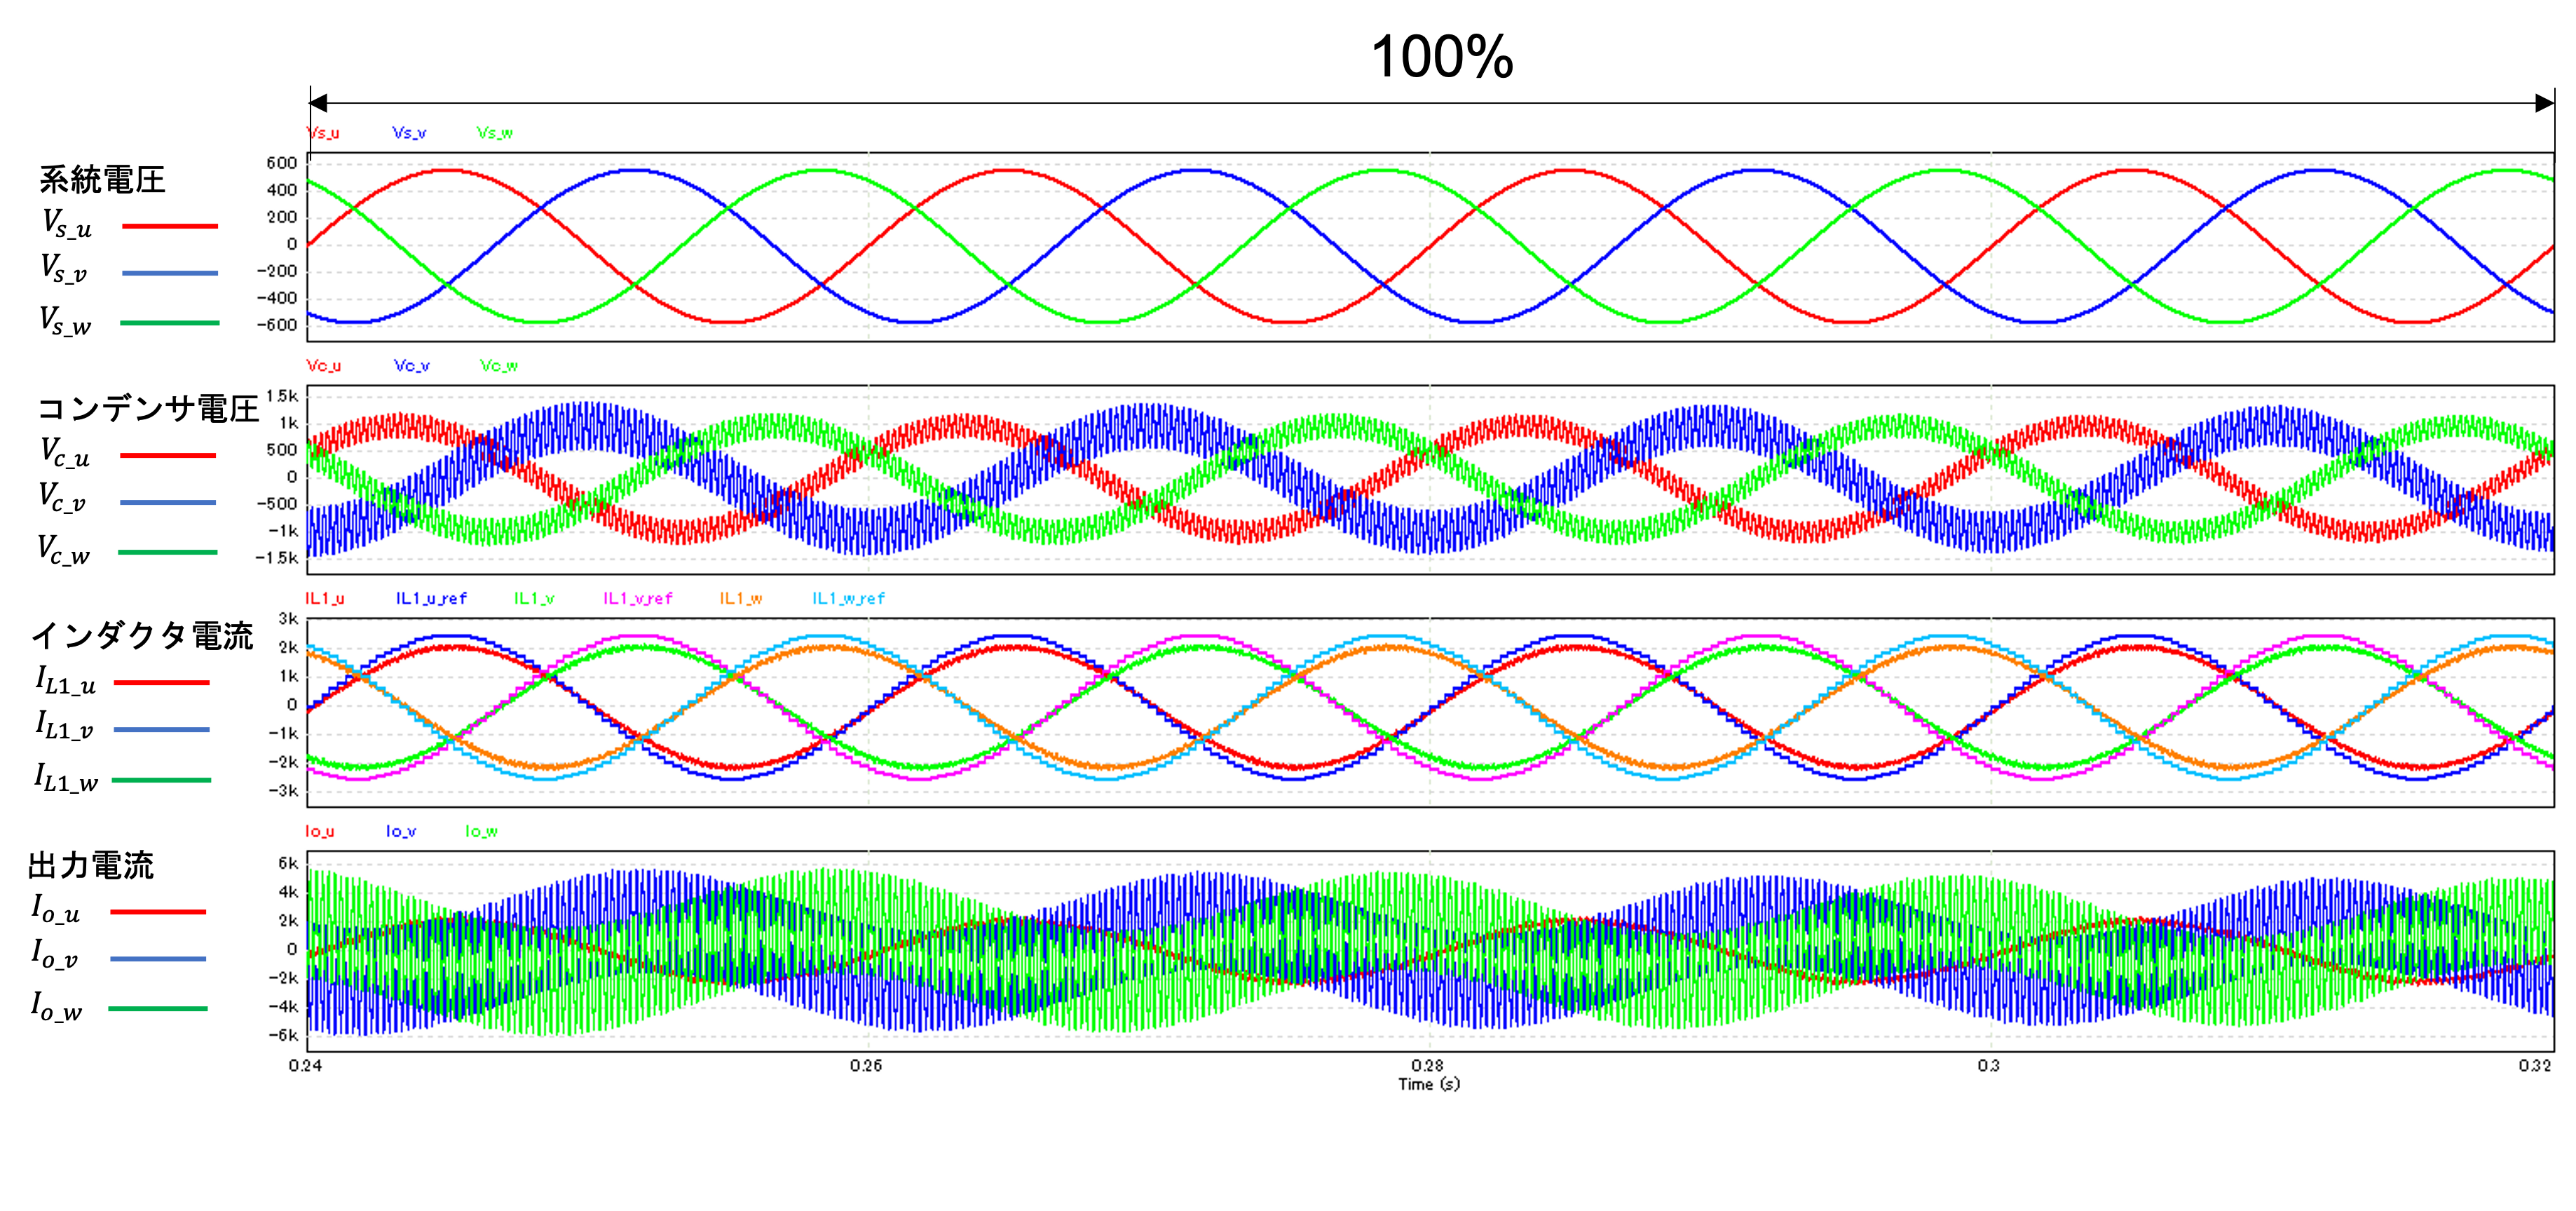
\includegraphics[width=140mm]{image/chapter3/Fig3.11.png}
    \caption{定常運転時(パターン2)}
    \label{Fig3.11}
\end{figure}

\begin{figure}[ht]
    \center
    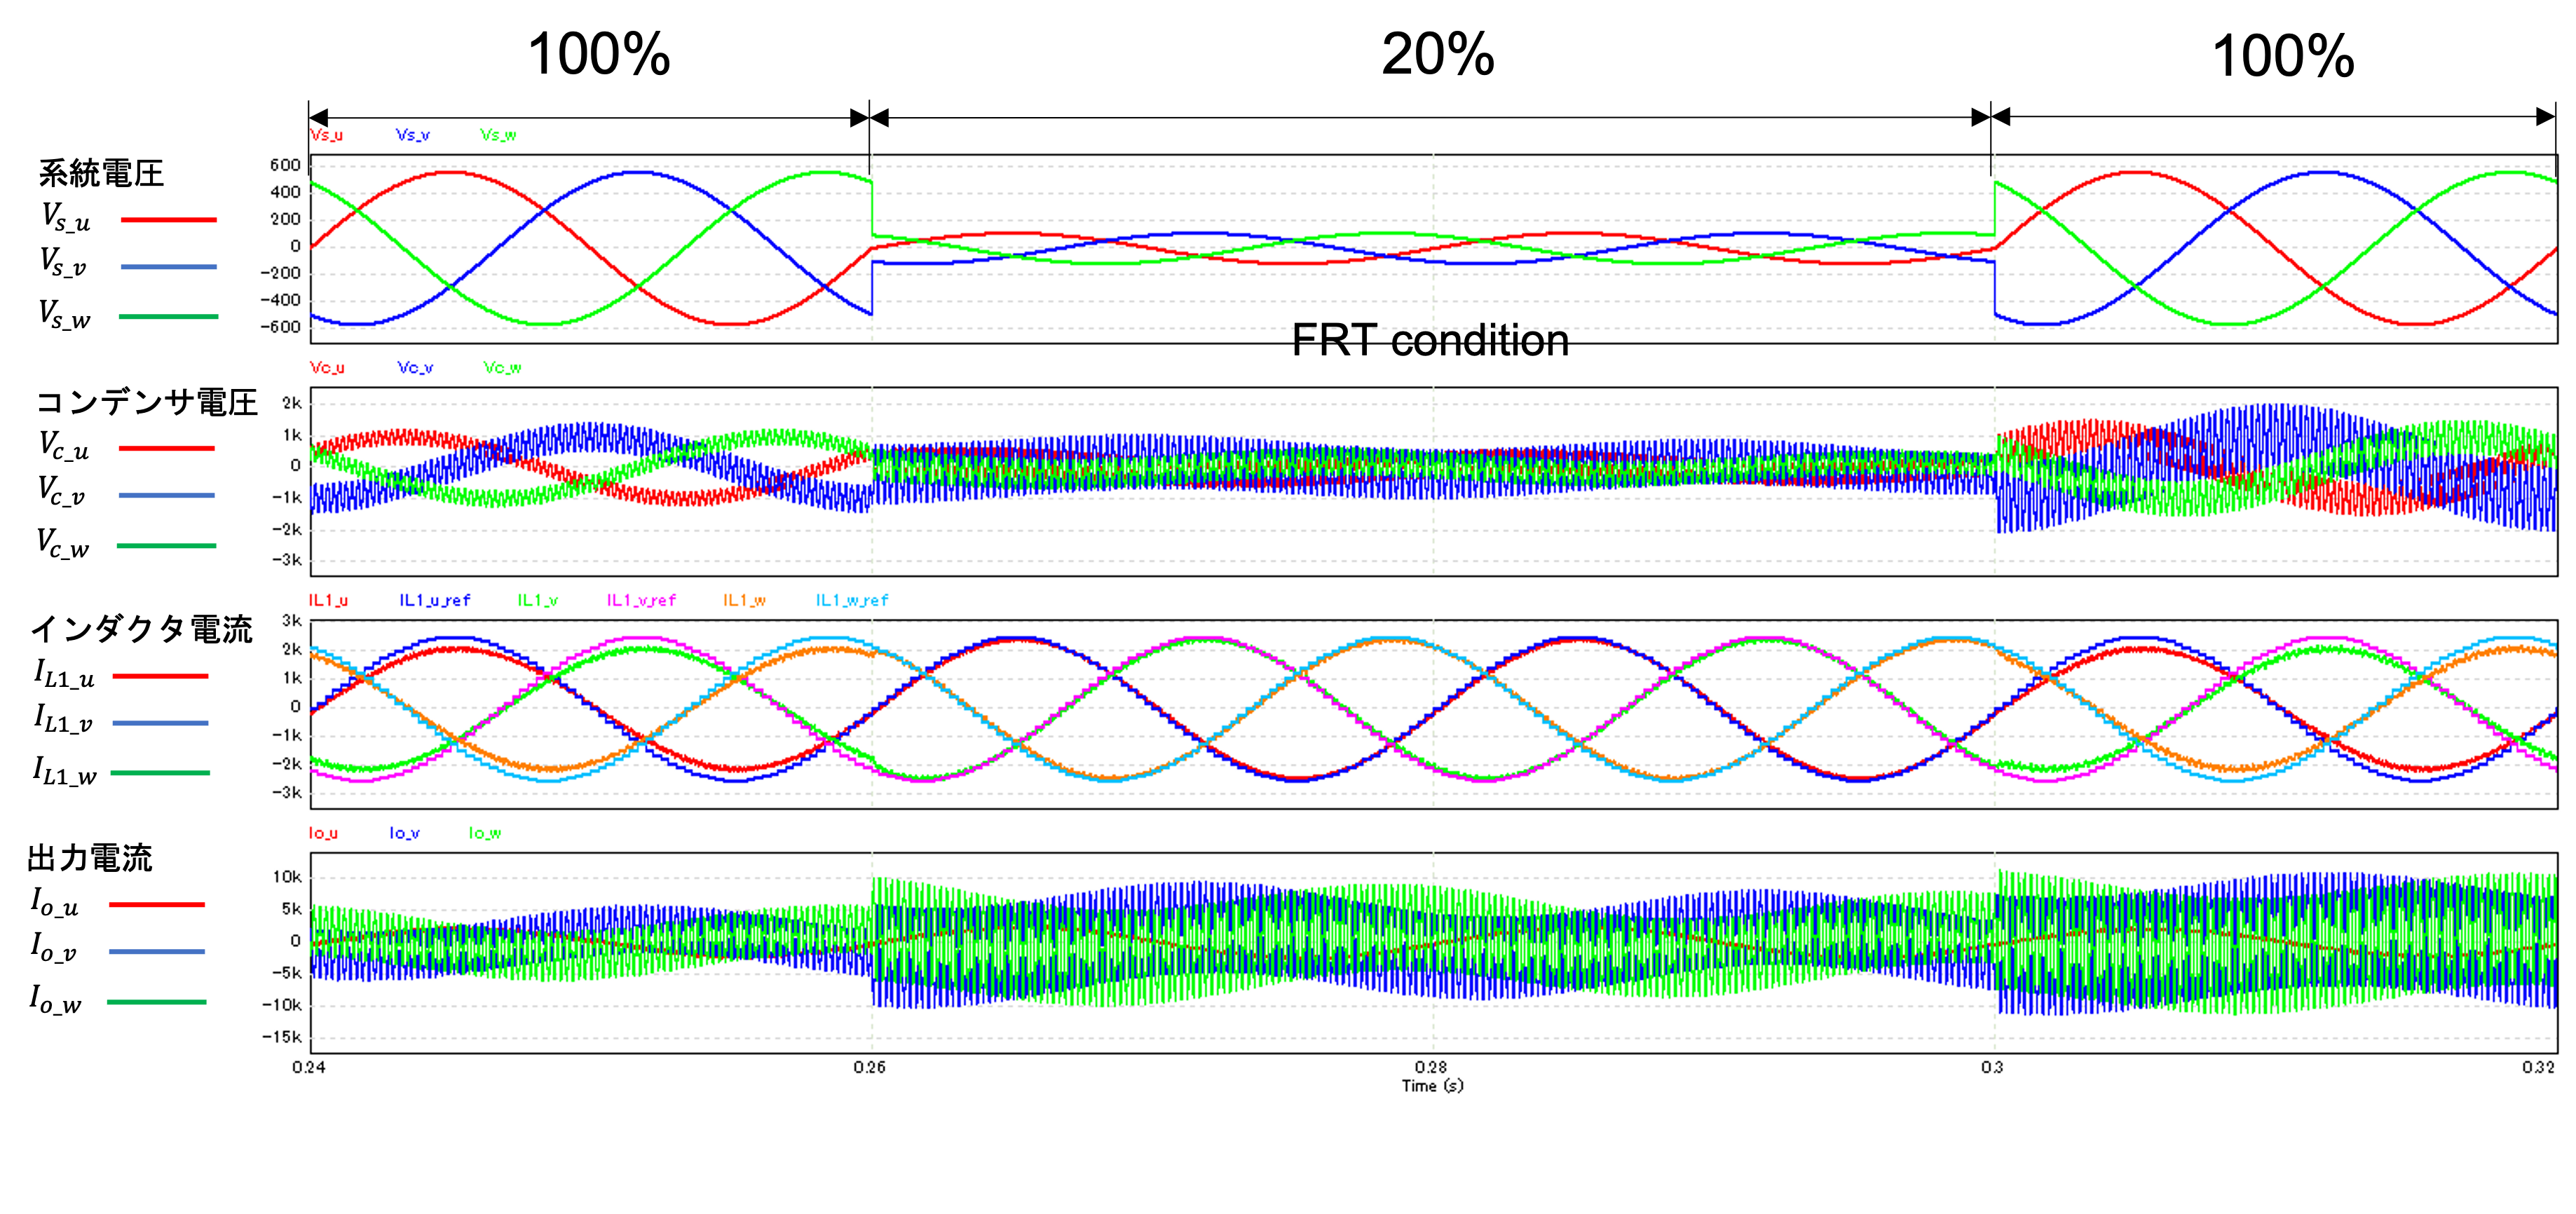
\includegraphics[width=140mm]{image/chapter3/Fig3.12.png}
    \caption{系統擾乱発生時(パターン2)}
    \label{Fig3.12}
\end{figure}

表\ref{Tab3.8}にシミュレーション結果を示す．
\newpage

\begin{table}[htb]
\centering
  \caption{シミュレーション結果}
  \begin{tabular}{c|c|c|c}  \hline\hline 
    \multirow{2}{*}{Condition}& \multicolumn{3}{|c}{THD [\%]} \\  \cline{2-4}
     & U相 & V相  & W相\\  \hline 
    定常時 & 2.09 & 2.29 & 2.31 \\ 
    系統擾乱発生時 & 1.16 & 1.98 & 1.08 \\ \hline
  \end{tabular}
  \label{Tab3.8}
\end{table}

表\ref{Tab3.8}から，定常運転時と系統擾乱発生時の場合において制御量であるインダクタ電流$I_{L1}$を制御することが出来ているわかる．また，定常運転時，系統擾乱発生時のTHDはFRT要件で定められている5\%を満たしていることがわかる．定常運転時に対して系統擾乱発生時でTHDがそれぞれU相で45\%減少，V相で14\%減少，W相で54\%減少していることがわかる．\\
さらに，コンデンサ電圧$V_{c}$，出力電流$I_{o}$でフィルタ共振を起こしていることが確認できた．\par
表\ref{Tab3.9}にシミュレーション結果の一覧を示す．

\begin{table}[htb]
 %\centering
 \footnotesize	
 \small
  \caption{シミュレーション結果の一覧}
  \begin{tabular}{ccc|c|c|c|c}  \hline\hline 
    \multicolumn{2}{c}{\multirow{2}{*}{Condition}}& \multicolumn{3}{|c}{Parameter} & \multicolumn{2}{|c}{THD[\%](U相)}\\ \cline{3-7}
    \multicolumn{2}{c|}{}  &  $L_{1}$ & $C$ & $L2$          & DC-SRDB &DC-MSSRDB \\ \cline{1-7}
    \multirow{2}{*}{ノミナル} &  \multicolumn{1}{|c|}{定常時} & \multirow{2}{*}{$51\mu $H} & \multirow{2}{*}{$995 \mu $F} & \multirow{2}{*}{$51\mu $H}  & 0.88\% & 0.89 \% \\
     & \multicolumn{1}{|c|}{系統擾乱} & & & & 0.77\% & 1.46 \% \\\cline{1-7}
    アンノミナル & \multicolumn{1}{|c|}{-} & - & - & - & - & - \\ 
    \multirow{2}{*}{パターン1} & \multicolumn{1}{|c|}{定常時} &\multirow{2}{*}{1.5 mH}&\multirow{2}{*}{2.0 mF}&\multirow{2}{*}{0.2 mH}&8.37\%&7.40\% \\ 
     &\multicolumn{1}{|c|}{系統擾乱}& & & &7.35\% &6.86\%\\ \cline{1-7}
    \multirow{2}{*}{パターン2} &\multicolumn{1}{|c|}{定常時} &\multirow{2}{*}{0.35 mH}&\multirow{2}{*}{$200 \mu$F}& \multirow{2}{*}{0.02 mH}& 18.4\% &2.09\%\\ 
     &\multicolumn{1}{|c|}{系統擾乱}& & & &28.9\%&1.16\% \\ \hline 
  \label{Tab3.9}
  \end{tabular}
\end{table}


表\ref{Tab3.9}は定常運転時・系統擾乱発生時において，ノミナル，アンノミナル時にDC-SRDB制御，DC-MSSRDB制御を適用した際にTHDがどのように変化するのかを表している．\par
表\ref{Tab3.9}より，ノミナル時は，定常時・系統擾乱発生時のいずれもDC-SRDB制御の方がDC-MSSRDB制御より優れた制御応答を示していることがわかる．一方で，アンノミナル時のパラメータを大きくしたパターン1において定常時，系統擾乱発生時のいずれにおいてもDC-MSSRDB制御の方が優れた制御応答を示していることがわかる．また，パラメータを小さくしたパターン2においても定常時，系統擾乱発生時のいずれの場合でもDC-MSSRDB制御の方が優れた応答性示している．\par
アンノミナル状態のパターン1より，パターン2の方がDC-MSSRDB制御を適用した効果が大きくなっていることがわかる．原因としては，図\ref{Fig3.5}から図\ref{Fig3.12}より，パターン1では，制御対象であるインダクタ電流$I_{L1}$を制御できていないということ，インダクタ，コンデンサのパラメータが制御対象の安定領域から外れたということなどが考えられる．

% 図
% \begin{figure}[htb]
%  \begin{center}
%  \includegraphics[width=50mm]
%  {image/image1}
%  \caption{}
%  \label{fig:}
%  \end{center}
% \end{figure}

% 表
% \begin{table}[htb]
%  \centering
%  \caption{}
%  \label{tab:}
%  \begin{tabular}{c|c}
%   \hline\hline
%   &\\ \hline
%   &\\ \hline
%  \end{tabular}
% \end{table}

% 式
% \begin{eqnarray}
%  a=b \nonumber \\
%  c=d \label{for:}
% \end{eqnarray}

% ソース
% \lstinputlisting[
%   caption=, 
%   label=list:
% ]
% {source/code1}


%Root main.tex
%---------------------------------------------------------------------------
%第2章　aaa
%---------------------------------------------------------------------------

\chapter{結論}
\label{chap:結論}

連系リアクトルを含まない制御モデルに対してデッドビート制御の指令値にノイズの模擬として，電流指令値の振幅に合わせた三角波を加えることで，システムの制御性がどのように変化するのかをシミュレーションによって検証した.その結果，デッドビート制御の指令値にノイズの模擬として，電流指令値の振幅に合わせた三角波を補正値として加えると特定の範囲で全高調波歪み率 (THD) の値が小さくなることを確認した.このことから，動的に指令値生成を行うことで，出力電流の制御性を改善できることが分かった.\par
今後の展望として，現在検証した範囲をより細かい範囲で検証し，制御性を向上し，制御性が向上した要因を分析する.また，事故時運転継続要件(FRT 要件)でデッドビート制御の指令値を変更することによって，システムの制御性がどのように変化するのかを検証する.さらに，繰り返し制御，AIを用いたニューラルネットワークの構築による出力電流の改善の検証を行なう．

%%Root main.tex
%---------------------------------------------------------------------------
%第2章　aaa
%---------------------------------------------------------------------------

\chapter{実機の基礎検証}
\label{chap:基礎検証}

\section{実機実装}
\subsection{ゲイン近似}
デッドビート制御ゲインの演算式に行列指数関数$e^{AT}$があり，式(\ref{for:SRDB式})のままでFPGAに書き込むと，膨大な演算量が発生し，大量のFPGAロジックセルを消費しまうため，拡張機能向けのロジックセル量が少なくなる．FPGAの演算量を低減するように，制御ゲインの結果をプロットし，近似式を求める．表\ref{for:GainPlot}に制御ゲインプロットする際の条件を示す．プロットした制御ゲイン$G^{-1}$,$G^{-1}F$それぞれを図\ref{fig:invG}，図\ref{fig:invGF}に示す．
\begin{table}[h]
 \center
 \caption{制御ゲインプロット用の条件}
 \label{for:GainPlot}
 \small
 \begin{tabular}{c|c} \hline \hline
  パラメータ定義		 & 値 		\\ \hline
  $d$軸インダクタンス($L_d$)[mH] & 6.9454	\\ \hline
  $q$軸インダクタンス($L_q$)[mH] & 8.8403	\\ \hline
  巻き線抵抗($R_L$)[$\Omega$]	 & 1.44		\\ \hline  
  キャリア周波数[Hz]		 & 5k		\\ \hline
  サンプリング周波数[Hz]	 & 1M		\\ \hline
  回転速度($N$)[rpm]		 & 0\textasciitilde2000		\\ \hline
 \end{tabular}
\end{table}
\begin{figure}[h]
 \center
 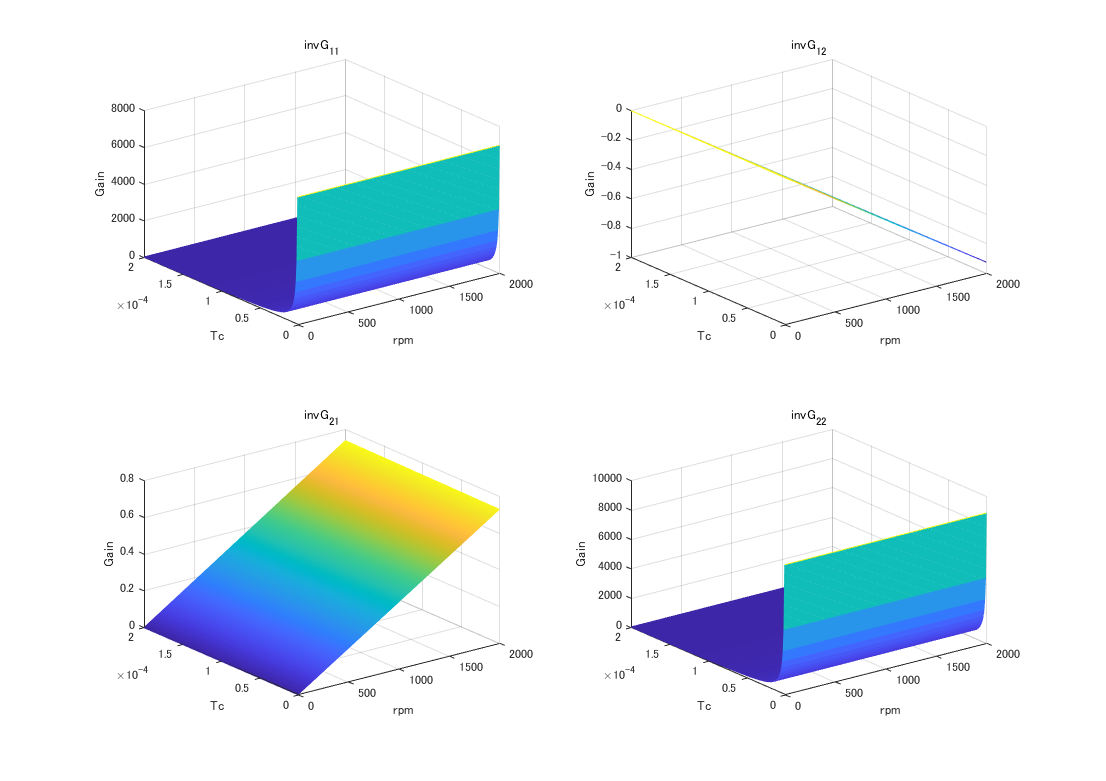
\includegraphics[width=120mm]{image/chapter5/invG.png}
 \caption{制御ゲイン$G^{-1}$}
 \label{fig:invG}
\end{figure}
\begin{figure}[h]
 \center
 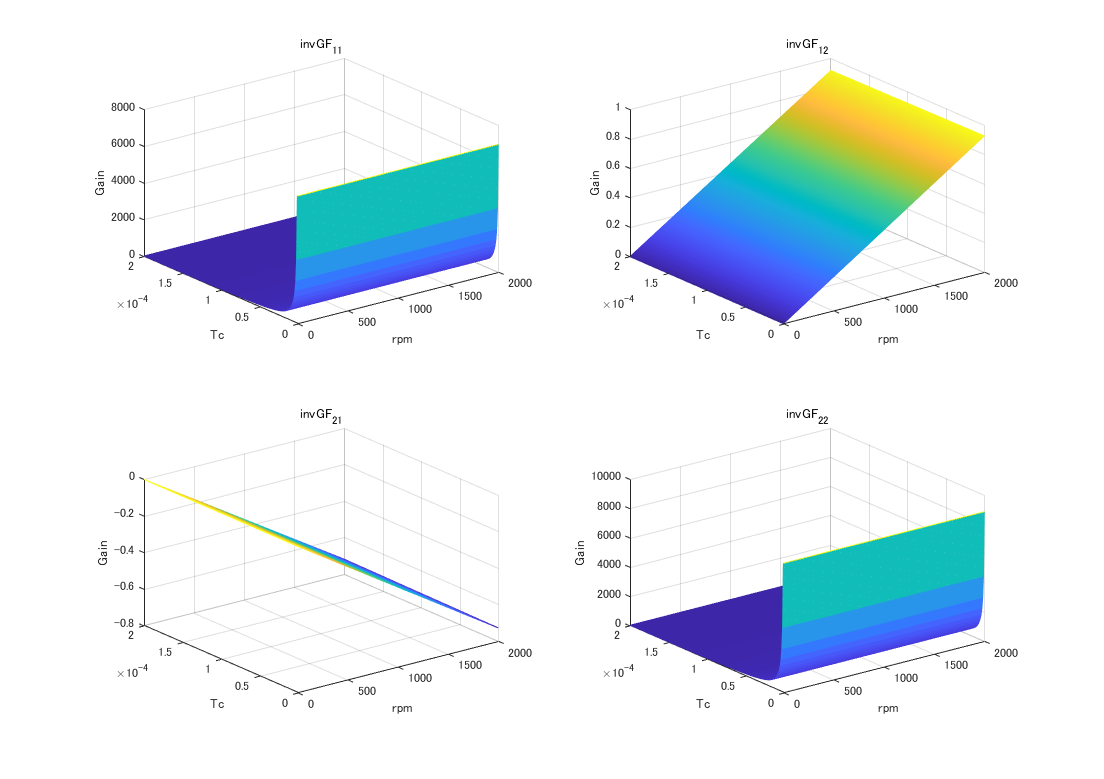
\includegraphics[width=120mm]{image/chapter5/invGF.png}
 \caption{制御ゲイン$G^{-1}F$}
 \label{fig:invGF}
\end{figure}

図\ref{fig:invG},\ref{fig:invGF}より，ゲイン$G^{-1}_{11}$,$G^{-1}_{22}$,$G^{-1}F_{11}$,$G^{-1}F_{22}$の変化はモータの回転数に依存しないことがわかったため，モータ回転を考慮しないで近似する．また，$T_c$が小さくなるとともに，ゲイン$G^{-1}_{11}$,$G^{-1}_{22}$,$G^{-1}F_{11}$,$G^{-1}F_{22}$が大きくなり，0\textasciitilde50$\mu s$の間，指数変化とみなされる．$\mu s$で急激な変化が起きる場合，FPGA演算にはオーバーフローが生じやすくなる．それ故，リミッタを設けて，上限値を上回ったら，上限値を出力する．今回，50$\mu s$のところにゲインリミッタを入れる．図\ref{fig:no_omega_Gain}にリミッタありおよびモータ回転を考慮しないゲイン$G^{-1}_{11}$,$G^{-1}_{22}$,$G^{-1}F_{11}$,$G^{-1}F_{22}$を示す．
\begin{figure}[h]
 \center
 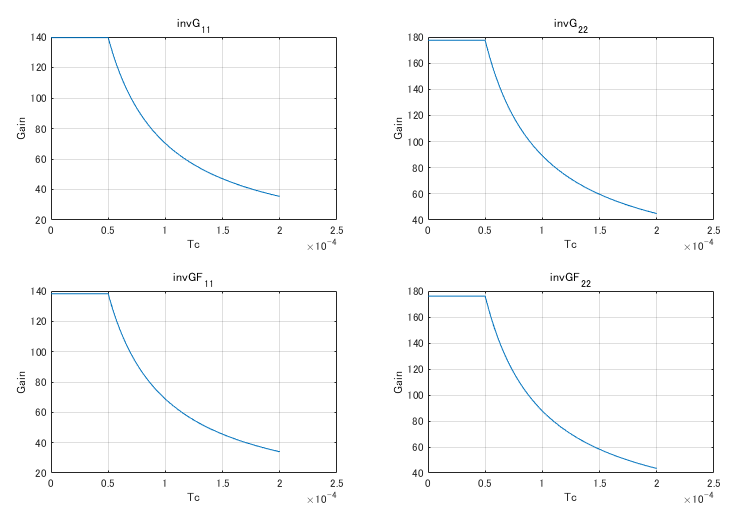
\includegraphics[width=105mm]{image/chapter5/limit_Gain.png}
 \caption{モータ回転を考慮しないゲイン}
 \label{fig:no_omega_Gain}
\end{figure}

$G^{-1}$,$G^{-1}F$の近似式は以下となる．
\begin{eqnarray}
 G^{-1}\left\{
 \begin{aligned}
    &G^{-1}_{11}=139.629(0<T_c<50\mu s)\\
    &G^{-1}_{11}=\frac{0.006944}{T_c}+0.7306(50<T_c<200\mu s)\\
    &G^{-1}_{12}=0.00287-0.0004657\omega-28.56T_c\\
    &G^{-1}_{21}=-0.00226-0.0003659\omega+22.44T_c\\
    &G^{-1}_{22}=177.527(0<T_c<50\mu s)\\
    &G^{-1}_{22}=\frac{0.008836}{T_c}+0.7283(50<T_c<200\mu s)
 \end{aligned}
 \right.
 \label{for:invG}
\end{eqnarray}
\begin{eqnarray}
 G^{-1}F\left\{
 \begin{aligned}
    &G^{-1}F_{11}=138.189(0<T_c<50\mu s)\\
    &G^{-1}F_{11}=\frac{0.00694}{T_c}-0.7094(50<T_c<200\mu s)\\
    &G^{-1}F_{12}=0.00287+0.00046\omega-28.56T_c\\
    &G^{-1}F_{21}=-0.00226-0.0003614\omega+22.44T_c\\
    &G^{-1}F_{22}=176.087(0<T_c<50\mu s)\\
    &G^{-1}F_{22}=\frac{0.008836}{T_c}-0.7117(50<T_c<200\mu s)
 \end{aligned}
 \right.
 \label{for:invGF}
\end{eqnarray}

式(\ref{for:invG}),(\ref{for:invGF})における$T_c$の初期値はキャリア周期と同じであり，1サンプリング毎にAD変換周期である1$\mu$sずつ減少させる．$\omega$はモータ角速度である．
\subsection{HDLコード生成}
開発周期の短縮、デバッグ作業の簡素化、コードのトレーサビリティ、早期検証などのことを実現するため，MATLAB/HDL Coderツールを利用する．HDLコード生成手順は主にSimulinkにおいてコードを生成するための回路作成、回路のシミュレーションおよび結果検証、固定小数点ツールでデータ型の最適化、HDLコード生成四つがある．コード生成のSimulinkを図\ref{fig:HDL_Simulink}に示す．
\begin{figure}[h]
 \center
 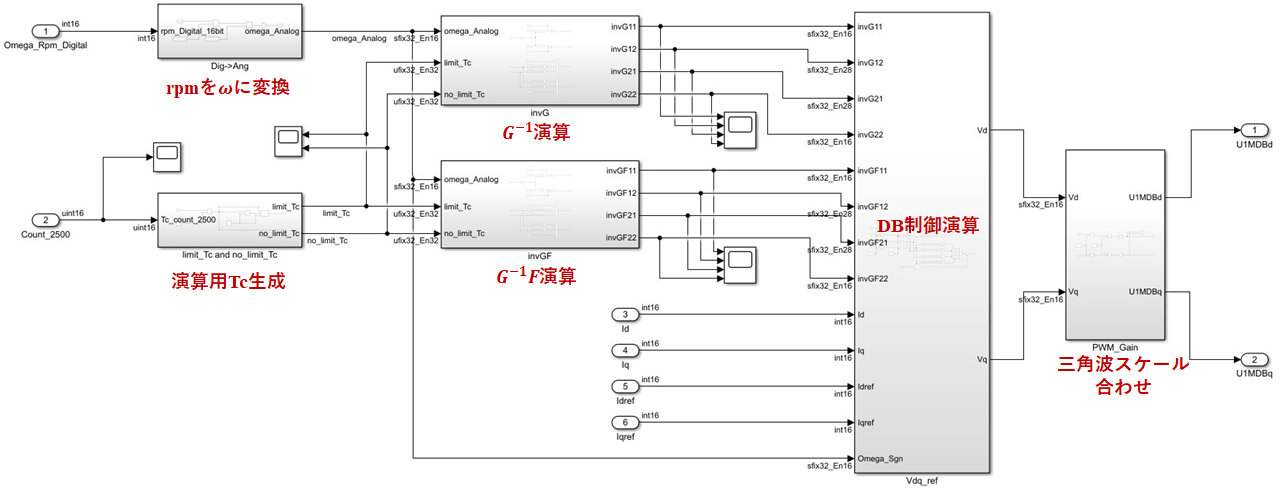
\includegraphics[width=135mm]{image/chapter5/HDL_Simulink.png}
 \caption{HDLコード生成のSimulinkモデル}
 \label{fig:HDL_Simulink}
\end{figure}

HDLコード生成回路による演算したゲインが正しいことを検証するため，シミュレーションを行い，図\ref{fig:Simulink_Gain}にシミュレーション波形示す．ただし，シミュレーション条件は表\ref{for:GainPlot}と同じである．

\begin{figure}[h]
 \center
 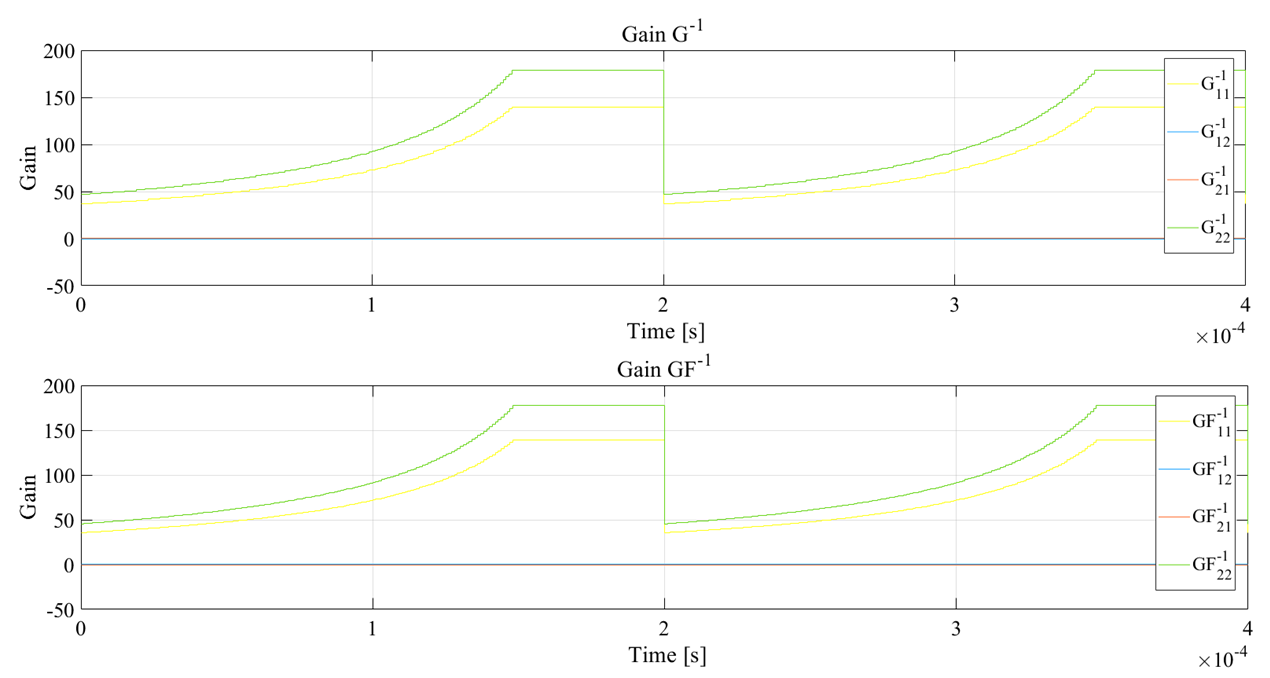
\includegraphics[width=130mm]{image/chapter5/HDL_Gain.png}
 \caption{近似ゲインの検証波形}
 \label{fig:Simulink_Gain}
\end{figure}

波形より，HDLコード生成回路による演算したゲインはゲイン近似で求めた結果が一致しており，回路が正しいと考えられる．シミュレーションを行う際，double型データを用いたが，FPGAに扱っているデータは固定小数点型のため，図\ref{fig:Fitting Tool}の固定小数点ツールによるデータ変換を行う．データ範囲も同時表示されるため，オーバーフロー、アンダーフローを無くすようにデータ型を調整する．
\begin{figure}[h]
 \center
 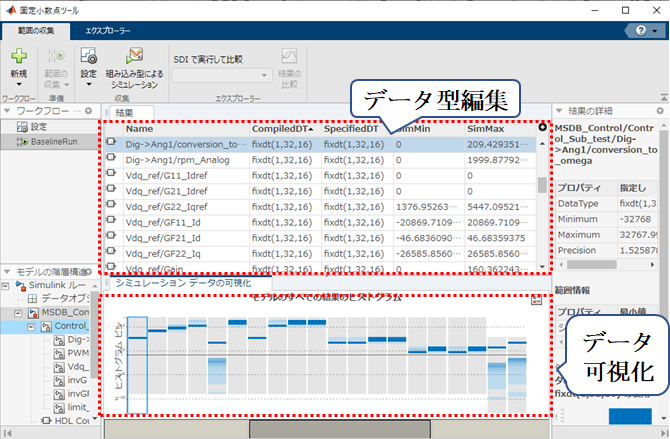
\includegraphics[width=120mm]{image/chapter5/Curve_Fitting_Tool.png}
 \caption{固定小数点ツール}
 \label{fig:Fitting Tool}
\end{figure}

調整したデータ型をSimulinkに適応し，HDL Coderツールでコード生成を行う．図\ref{fig:MSDB_HDL}に生成したHDLモジュール構成を示す．
\begin{figure}[h]
 \center
 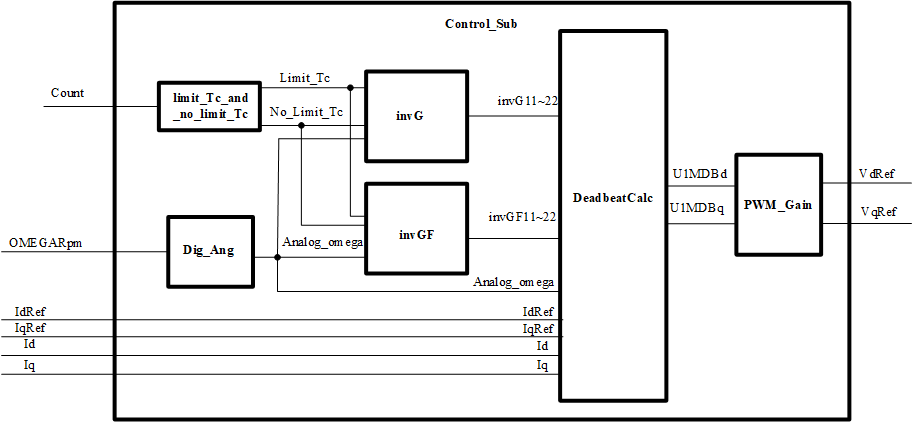
\includegraphics[width=120mm]{image/chapter5/MSDB_HDL.png}
 \caption{生成したHDLモジュール構成}
 \label{fig:MSDB_HDL}
\end{figure}

図\ref{fig:MSDB_HDL}に示しているように，$T_c$場合分けモジュール・回転速度演算モジュールはホールドあり、なし$T_c$と$rad/s$である回転速度を算出し，ゲイン演算モジュールに渡す．操作量演算モジュールは実電流、指令電流および制御ゲインを受信し，$dq$軸操作量を出力する．操作量と三角波スケールを合わせるため，正規化モジュールを利用する．


\newpage
\section{実機結果}
\subsection{実機構成および検証条件}
生成したHDLコードの正確性を検証する実機構成を図\ref{fig:real systeam}に示す．

\begin{figure}[h]
 \center
 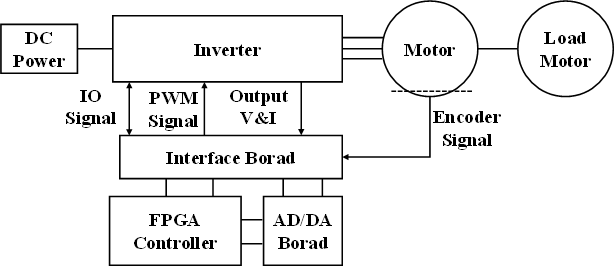
\includegraphics[width=110mm]{image/chapter5/real_systeam.png}
 \caption{コード検証の実機構成}
 \label{fig:real systeam}
\end{figure}

直流電源はインバータに200V電圧を提供する．インバータにおけるスイッチング素子はFPGAから送信されたPWM信号によってON/OFFし，三相交流を出力する．エンコーダで計測した角速度および回転角がインタフェースボードを通って，FPGAコントローラに送信される．電流センサによる取得した電流がインタフェースボード、AD変換基板を介してFPGAコントローラにフィードバックする．HDL開発ソフトQuartusを用いて生成したコードをFPGAコントローラに実装する．実機検証の条件を表\ref{for:実機条件}に示す．

\begin{table}[h]
 \center
 \caption{制御ゲインプロット用の条件}
 \label{for:実機条件}
 \small
 \begin{tabular}{c|c} \hline \hline
     条件の定義		 & 値 		\\ \hline
     回転速度($N$)[rpm]	 & 200		\\ \hline
     キャリア周波数[Hz]		 & 5k	\\ \hline
     サンプリング周波数[Hz]	 & 1M		\\ \hline
     $d$軸指令電流($i_{dref}$)[A]	 & 0		\\ \hline
     $q$軸指令電流($i_{qref}$)[A]	 & 0→1.5	\\ \hline
 \end{tabular}
\end{table}

\newpage
\subsection{実機波形}
図\ref{fig:MSDB_Real_Ans}にMSDB制御の実機波形，図\ref{fig:MSDB_Real_Big}にdq軸立ち上がり部分の拡大を示す．
\begin{figure}[h]
 \center
 \includegraphics[width=140mm]{image/chapter5/Real_dq.png}
 \caption{MSDB制御の$dq$軸電流}
 \label{fig:MSDB_Real_Ans}
\end{figure}
\begin{figure}[h]
 \center
 \includegraphics[width=140mm]{image/chapter5/Real_dq_big.png}
 \caption{$dq$軸電流の拡大図}
 \label{fig:MSDB_Real_Big}
\end{figure}

$dq$軸実電流波形より，$d$軸実電流が指令電流0Aに到達するまでの時間は約202$\mu s$であり，その後，目標電流0Aに追従している．$q$軸実電流が目標電流1.5Aに到達するまでの時間は約200$\mu$sである．また，$d,q$軸実電流それぞれのリップル率は11.3$\%$,16.4$\%$であることがわかる．$dq$軸電流はいずれも1キャリア程度で指令値に追従したため，実機結果とシミュレーション結果が一致しており，生成したコードの正確性を検証できた．

% 図
% \begin{figure}[htb]
%  \begin{center}
%  \includegraphics[width=50mm]
%  {image/image1}
%  \caption{}
%  \label{fig:}
%  \end{center}
% \end{figure}

% 表
% \begin{table}[htb]
%  \centering
%  \caption{}
%  \label{tab:}
%  \begin{tabular}{c|c}
%   \hline\hline
%   &\\ \hline
%   &\\ \hline
%  \end{tabular}
% \end{table}

% 式
% \begin{eqnarray}
%  a=b \nonumber \\
%  c=d \label{for:}
% \end{eqnarray}

% ソース
% \lstinputlisting[
%   caption=, 
%   label=list:
% ]
% {source/code1}
%%Root main.tex
%---------------------------------------------------------------------------
%第2章　aaa
%---------------------------------------------------------------------------

\chapter{結論}
\label{chap:結論}
　本研究では，USPMコントローラを用いて50MHz MSDB制御を行うことにより，高性能のPMSMドライブシステムを実現することを目的とし，先行研究で提案されたSRDB制御、MSDB制御について学び，MSDB制御のシミュレーションを行った．従来のMATLAB Coderでモータモデルの作成のようなシミュレーション手法と比べ，MATLAB/Simscapeを用いたことで，PMSMドライブシステムの物理モデルを素早く作成できた．Cureve Fitting Tool、Fixed-Point Tool、HDL Coder拡張機能により，実装データの最適化、開発周期の短縮化、デバッグの簡素化を実現した．また，実機波形の結果，生成したMSDB制御コードの正確性を検証できた．今後，USPMを用いた新たな実験環境に50MHz MSDB制御コードを実装し，検証を行う．

%%Root main.tex
%---------------------------------------------------------------------------
%第2章　aaa
%---------------------------------------------------------------------------

\chapter{aaa}
\label{chap:aaa}

\section{bbb}

\subsection{ccc}

% 図
% \begin{figure}[htb]
%  \begin{center}
%  \includegraphics[width=50mm]
%  {imege/image1}
%  \caption{}
%  \label{fig:}
%  \end{center}
% \end{figure}

% 表
% \begin{table}[htb]
%  \centering
%  \caption{}
%  \label{tab:}
%  \begin{tabular}{c|c}
%   \hline\hline
%   &\\ \hline
%   &\\ \hline
%  \end{tabular}
% \end{table}

% 式
% \begin{eqnarray}
%  a=b \nonumber \\
%  c=d \label{for:}
% \end{eqnarray}

% ソース
% \lstinputlisting[
%   caption=, 
%   label=list:
% ]
% {source/code1}



%---------------------------------------------------------------------------
%　参考文献
%---------------------------------------------------------------------------
\begin{thebibliography}{10}
 \bibitem{1}経済産業省・資源エネルギー庁：”第2部エネルギー動向第１章国内エネルギー動向第1説エネルギー需供の動向”，\\https://www.enecho.meti.go.jp/about/whitepaper/2013html/2-1-1.html，閲日時2023年2月13日21:00.
 \bibitem{2}環境省：「令和3年度版環境白書循環型社会白書/生物多様性白書」
 \bibitem{3}河村篤男，”現代パワーエレクトロニクス”，数理工学社，2005
 \bibitem{4}角田秀夫，”PLLの基本と応用”，東京電機大学出版局，1978
\bibitem{5}石原清志，河村篤男："DSPによる実時間出力合成形三相PWMインバータ"電気学会D，110巻6号，平成2年
\bibitem{6}川島加也：”Universal Smart Power Module(USPM)コントローラを用いた系統連系システム”，令和3年度東京電機大学卒業論文
 \bibitem{7}加藤遼子：”系統連系用マルチレベルインバータにおける外乱補償型デッドビート制御系の構築”，令和3年度東京電機大学修士論文
\bibitem{8}廣惠大輔：”高性能FPGAコントローラによる50MHzマルチサンプリングデッドビート制御”，令和2年度東京電機大学卒業論文
\bibitem{9}細山田悠：”高速High/LOWパルス動作を実現する3相インターリーブDC/DCコンバータの制御手法の検討”，令和3年度横浜国立大学博士論文
\bibitem{10}小原秀嶺：”フライングキャパシタマルチレベルコンバータによる電力変換器の波形改善および高パワー密度化に関する研究”，千葉大学2015年度博士論文
\end{thebibliography}
 
%---------------------------------------------------------------------------
%------------------　　　　　　 質問応答　　　 　　　　　 ------------------
%---------------------------------------------------------------------------
\chapter*{質問応答}
\addcontentsline{toc}{chapter}{質問応答}{
Q1．デッドビート制御とはなんですか？(石川先生)\\
A1.1キャリア毎に状態量を指令値に追従させる制御．\\
\\
Q2．デッドビート制御はハイゲインになりやすくハイゲインフィードバックとなった場合，実際のシステムに実装することができないという問題が発生する可能性があるがどう対応するのか？(石川先生)\\
A2.オブザーバを制御に実装したり，ノイズや高調波が原因であればフィルタを更に追加実装する．\\
\\
Q3.デッドビート制御はパラメータだけではなく，サンプリング周期が制御応答に影響を与えるが，サンプリング周期を変えた場合の検証を行う予定はあるのか？(石川先生)\\
A3.行う予定である．\\
\\ 
Q4.パラメータは何に基づいて決めた値であるのか？(石川先生)\\
A4.実際のシステムを参考にして決めた値とシミュレーションによって決めた値がある．
\\
\\
・コメント(釜道先生)\\
1.発表の際には結果をより具体的に発表した方が良いと思う．\\
2.アンノミナル時にはフィルタ共振が発生しない状態で制御できていないので，パラメータを変更したときに応答がどのように変化するか追加で検証する必要があると思う．


}


%---------------------------------------------------------------------------
%------------------　　　　　　 　　謝辞　　　 　　　　　 ------------------
%---------------------------------------------------------------------------
\chapter*{謝辞}
\addcontentsline{toc}{chapter}{謝辞}{
　本研究を行うに当たって，適切な指導，様々な意義深い提案，深い御示唆をおくりました．東京電機大学ロボット・メカトロニクス学科の横山智紀教授に深くお礼申し上げます．また，研究を進めるにあたりご助言を頂いたロボット・メカトロニクス学科の先生方，同期の方々に心から感謝いたします．
\begin{flushright}
19FR053 窪慎之助
\end{flushright}
}


%---------------------------------------------------------------------------
%---------------------　   　     付録   　　　 　 -------------------------
%---------------------------------------------------------------------------
%\newpage
%\appendix
%\part*{\Huge 付録}
\addcontentsline{toc}{part}{付録}
%Root main.tex
%---------------------------------------------------------------------------
%付録A　付録
%---------------------------------------------------------------------------
% --- プリアンブルに追加してください ---
% \usepackage{float}
% \usepackage{listings}
% ----------------------------------

%Root main.tex
%---------------------------------------------------------------------------
%付録A　付録
%---------------------------------------------------------------------------

\chapter{PSIMを用いたシミュレーション}
\thispagestyle{fancy}
\label{chap:MATLAB}
本研究ではプラス株式会社のPSIMを用いてシミュレーションを行った．PSIMではパワーエレクトロニクスの解析，制御系回路設計，インバータ，モータドライブの研究に対して有効なシミュレーション環境が提供されている．シミュレーションにおける制御部分は，Cブロックに書き込むことによって実装することができる．表\ref{tabA.1}にPSIMの実行環境を示す．

\begin{table}[H]
    \centering
    \caption{PSIMの実行環境}
    \label{tabA.1}
    \small
    \begin{tabular}{c|c} \hline \hline
        実行OS    &   ソフトバージョン    \\ \hline
        Windows11    & PSIM 2025a   \\ \hline
    \end{tabular}
\end{table}

表\ref{tabA.2}に本研究で使用したPSIMの実行ファイル名，保存場所を示す．

\begin{table}[H]
    \centering
    \caption{ファイル情報}
    \label{tabA.2}
    \small
    \begin{tabular}{l|l} \hline \hline
        実行ファイル名  & TMEIC\_LC\_main\_疑似dq.psimsch \\
                        & CCBPF.psimsch \\ \hline
        保存場所        & 「box」/「0-横山研究室資料共有フォルダ」/「ミーティング資料」/「系統」\\
                        & /「2025年度」/「yamazaki」/「卒論psimファイル」 \\ \hline
    \end{tabular}
\end{table}

本検証で使用したシミュレーションファイルは，TMEIC\_LC\_main\_疑似dq.psimschとCCBPF.psimschのみである．

\section{疑似dq変換のシミュレーション}
図\ref{FigA.1}に定常運転時の連携リアクトルなし三相系統連系システムを主回路図を示す．

\begin{figure}[H]
    \centering
    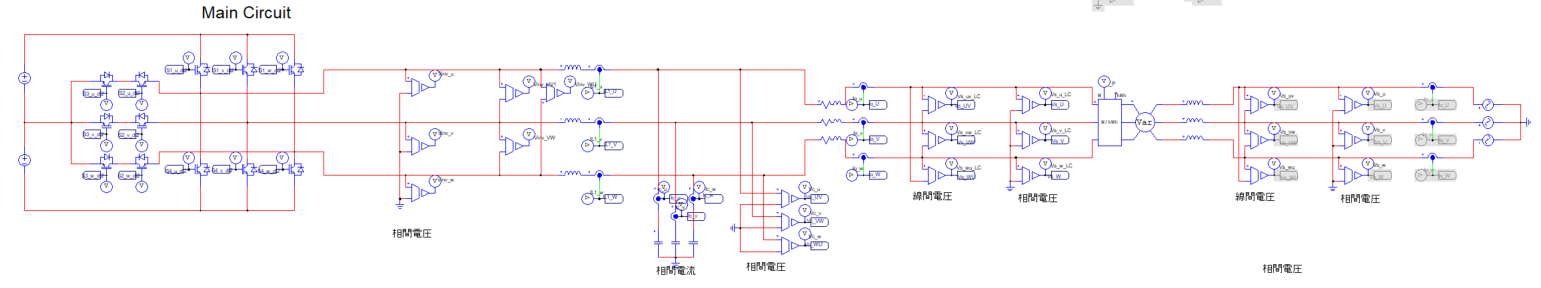
\includegraphics[width=140mm]{image/2025/1.png}
    \caption{定常運転時の連携リアクトルなし三相系統連系システムを主回路図}
    \label{FigA.1}
\end{figure}

図\ref{FigA.1}について，系統システムの制御に用いる状態変数の電流，電圧はそれぞれセンサから値を取得，もしくは数値計算によって導出する．
図\ref{FigA.2}に制御と状態変数のホールドを行うモジュールを示す．

\begin{figure}[H]
    \centering
    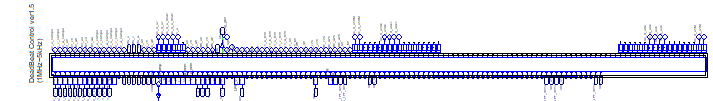
\includegraphics[width=140mm]{image/2025/2.png}
    \caption{制御と状態変数のホールドを行うモジュール}
    \label{FigA.2}
\end{figure}

図\ref{FigA.2}のCブロックでは，電流指令値の生成，デッドビート制御，パルス指令値の生成などを行なっている．
図\ref{FigA.4}に三角波比較のモジュールを示す．

\begin{figure}[H]
    \centering
    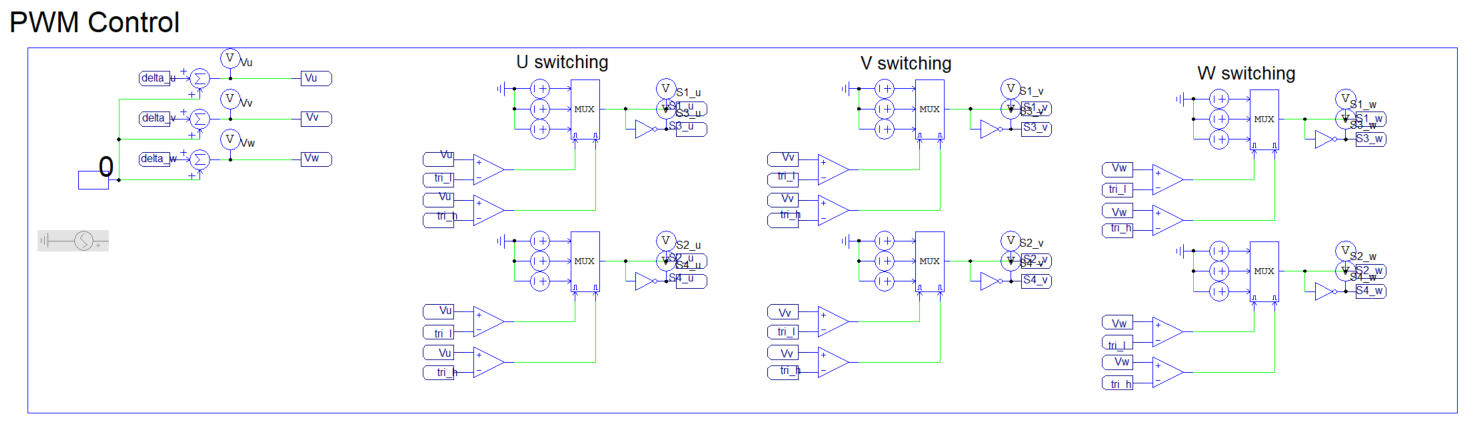
\includegraphics[width=80mm]{image/2025/3.png}
    \caption{三角波比較のモジュール}
    \label{FigA.4}
\end{figure}

図\ref{FigA.4}では，Cブロックで生成したU相のパルス$u_{u}$，V相のパルス指令値$u_{v}$，W相のパルス指令値$u_{w}$について三角波比較を行い，インバータのゲート信号を生成する．図\ref{FigA.5}にデッドタイム生成モジュールを示す．

\begin{figure}[H]
    \centering
    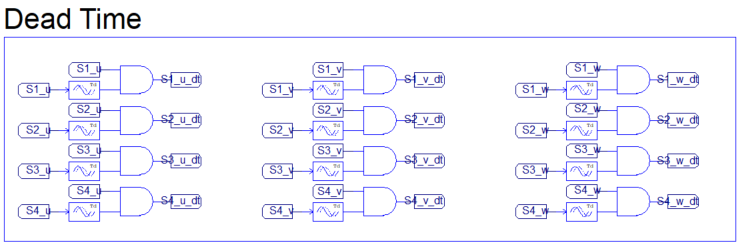
\includegraphics[width=140mm]{image/2025/4.png}
    \caption{デッドタイム生成モジュール}
    \label{FigA.5}
\end{figure}

図\ref{FigA.5}では，三角波比較により生成したゲート信号に対してデッドタイム処理を行うことで，インバータの各レグのアームが同時にONになるのを防ぐ処理を行う．

図\ref{FigA.6}にパラメータを示す．

\begin{figure}[H]
    \centering
    
\includegraphics[width=60mm]{image/appendixA/FigA.6.png}
    \caption{パラメータファイル}
    \label{FigA.6}
\end{figure}

図\ref{FigA.6}は，回路のパラメータやキャリア周期，サンプリング周期などを書き込むファイルである．

図\ref{FigA.7}に疑似dq変換の3サンプリング取得モジュールを示す．
\begin{figure}[H]
    \centering
    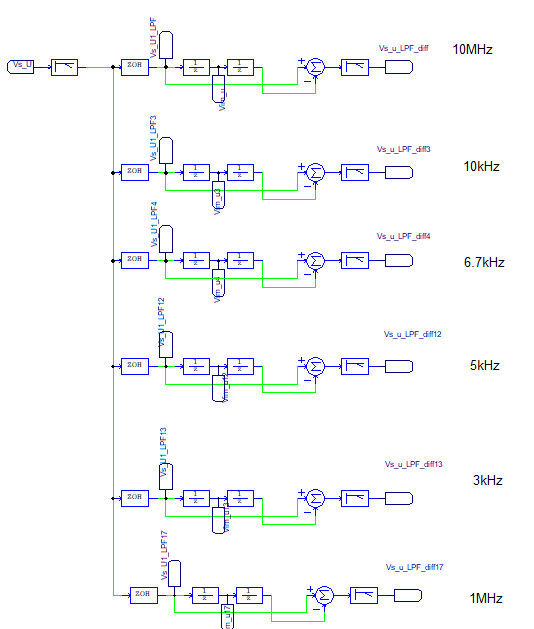
\includegraphics[width=80mm]{image/2025/5.png}
    \caption{疑似dq変換の3サンプリング取得モジュール}
    \label{FigA.7}
\end{figure}

図\ref{FigA.7}では，系統電圧をセンサにより取得し，零次ホールドによりサンプリング周波数でホールドする．
ホールドした後のデータを1サンプル目とする．次に単位遅れブロックにより1サンプル遅らせることで2サンプル目を生成する．
2サンプル目を虚軸のサンプリングデータとする．
さらにもう一度単位遅れブロックにより1サンプル遅らせることで3サンプル目を生成する．
このようにして，3サンプリング分の系統電圧のデータを取得する．
1サンプル目と3サンプル目のデータの差分をとる．

\section{複素係数フィルタのシミュレーション}
図\ref{FigA.8}に複素係数フィルタモジュールを示す．

\begin{figure}[H]
    \centering
    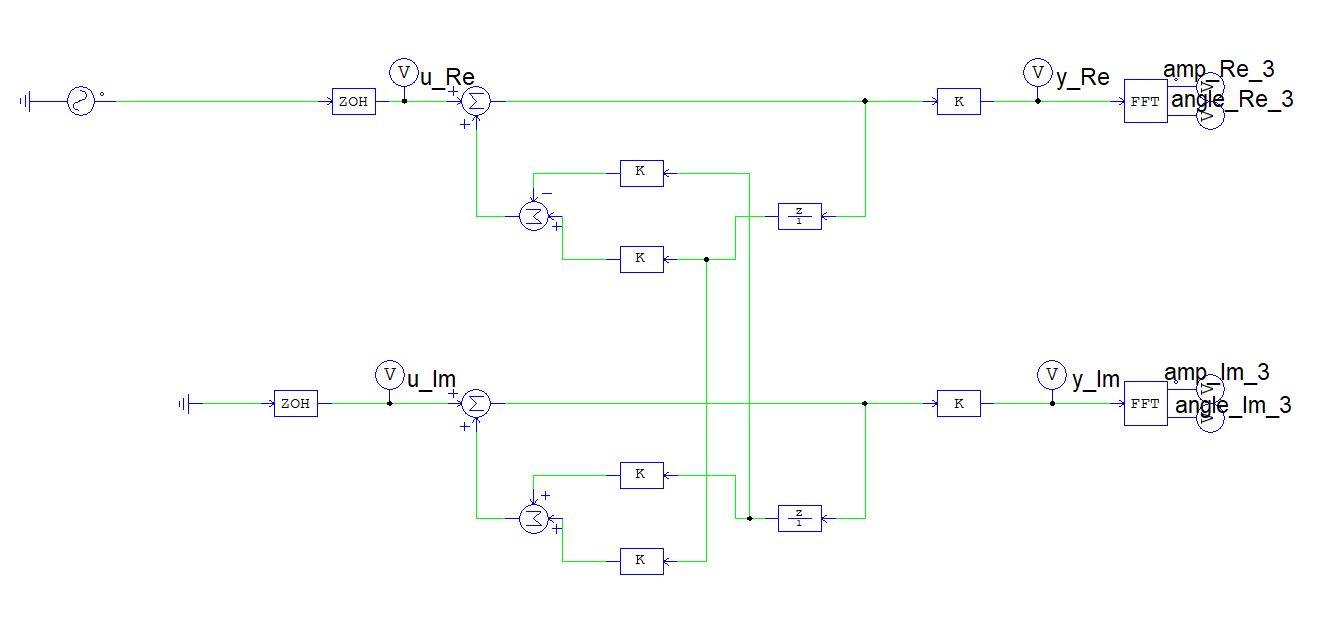
\includegraphics[width=140mm]{image/2025/6.png}
    \caption{複素係数フィルタモジュール}
    \label{FigA.8}
\end{figure}

図\ref{FigA.8}では，上部を実数部，下部を虚数部としている．入力電圧は実部のみに入力信号を入力している．
複素係数フィルタの出力は，上部に実部の出力を，下部に虚数部の出力を出力している．
PSIMでは虚数演算ができないため，実部と虚部を分けて計算する必要がある．

\section{DC-MSSRDB\_Control}
連携リアクトルなし三相系統連系システムにおけるプログラムリストをソースコード\ref{lisA.1}に示す．

\lstinputlisting[
    language=C,
    caption={DC-MSSRDB\_Control},
    label={lisA.1},
    basicstyle=\small\ttfamily,
    frame=single,
    breaklines=true
]{image/2025/lisA.1.c}
%%Root main.tex
%---------------------------------------------------------------------------
%付録B　付録
%----------------------------------------------------------------------------
\chapter{生成したHDLコードの仕様}
\thispagestyle{fancy}
\label{chap:コード}
\section{MSDB\_Control}
トップモジュール(Simulink全体)であり，入出力の信号名、ビット数などを定義している．入出力を表\ref{for:MSDB_Control}に示す．
\begin{table}[h]
 \center
 \caption{MSDB\_Controlポート一覧}
 \label{for:MSDB_Control}
 \small
 \begin{tabular}{c|c|c|c} \hline \hline
  信号名            &   方向    &   bit幅   &   説明   \\ \hline
  Omega\_Rpm\_Digital &   In      &   16      &   モータ回転数   \\ \hline
  Count\_2500       &   In      &   16      &   カウンタ信号   \\ \hline
  I\_d              &   In      &   16      &   d軸実電流   \\ \hline
  I\_q              &   In      &   16      &   q軸実電流   \\ \hline
  I\_dref           &   In      &   16      &   d軸指令電流   \\ \hline
  I\_qref           &   In      &   16      &   q軸指令電流   \\ \hline
  Vd                &   Out     &   16      &   d軸操作量   \\ \hline
  Vq                &   Out     &   16      &   q軸操作量   \\ \hline
 \end{tabular}
\end{table}

%\inputminted{vhdl}{image/appendixC/MSDB_Control.vhd}
\begin{center}
\label{lisC.1}
    ソースコードC.1：DC-MSSRDB\_Control
\lstinputlisting[language=VHDL]{image/appendixC/MSDB_Control.vhd}
\end{center}
%%%%%%%%%%%%%%%%%%%%%%%%%%%%%%%%%%%%%%%%%%%%%%%%%%%%%%%%%%%%%%%%%%%%%%%%%%%%%%%%%%%%%%
%\include{appendix/appendixC}


%---------------------------------------------------------------------------
%-----------------------　　    　　End　 　　　　　 -----------------------
%---------------------------------------------------------------------------
\end{document}
